% Standalone build of the HyperAVNet methodology and results sections.
% To use in a full paper: copy sections/, figures/, tables/ and refs.bib, then
%   % ============================================================================
%  Methodology -- HyperAVNet.  Self-contained: % ============================================================================
%  Methodology -- HyperAVNet.  Self-contained: % ============================================================================
%  Methodology -- HyperAVNet.  Self-contained: \input{sections/method} in any paper.
%  Requires: amsmath, amssymb, bm, booktabs, graphicx, (cleveref optional).
% ============================================================================
\section{Methodology}
\label{sec:method}

\subsection{Problem formulation}
\label{sec:problem}
Each sample of AV-FFIA is a synchronised two-second clip $(\mathbf{x}^{a}, \mathbf{X}^{v})$, where
$\mathbf{x}^{a}\in\mathbb{R}^{L}$ is the hydrophone waveform ($L = 2f_s$, $f_s = 64$\,kHz) and
$\mathbf{X}^{v}\in[0,1]^{3\times T\times H\times W}$ holds $T$ RGB frames sampled uniformly from the
overhead camera. The label $y\in\mathcal{Y}=\{\textsc{None},\textsc{Weak},\textsc{Medium},\textsc{Strong}\}$
is the feeding intensity. We learn $f_{\theta}:(\mathbf{x}^{a},\mathbf{X}^{v})\mapsto\mathbf{p}\in\Delta^{|\mathcal{Y}|-1}$ with
two goals that pull in opposite directions: high accuracy, robust to the acoustic and visual
corruptions typical of aquaculture (bubbles, pumps, low light, reflections), and a small
parameter and compute budget for on-site deployment.

HyperAVNet (Fig.~\ref{fig:overview}) has four parts. Two hypercomplex backbones map each modality to a
hierarchy of \emph{stage tokens} (Sec.~\ref{sec:backbones}). A set of shared \emph{bottleneck tokens}
is updated by hypercomplex component fusion (HCF) blocks attached at a configurable subset of
stages, with zero-initialised cross-modal feedback into both streams (Secs.~\ref{sec:hcf},~\ref{sec:schedule}).
Fused and unimodal heads produce the predictions (Sec.~\ref{sec:heads}). The model is trained with a
multi-level distillation objective from a pretrained audio-visual teacher (Sec.~\ref{sec:objective}).

\begin{figure*}[t]
  \centering
  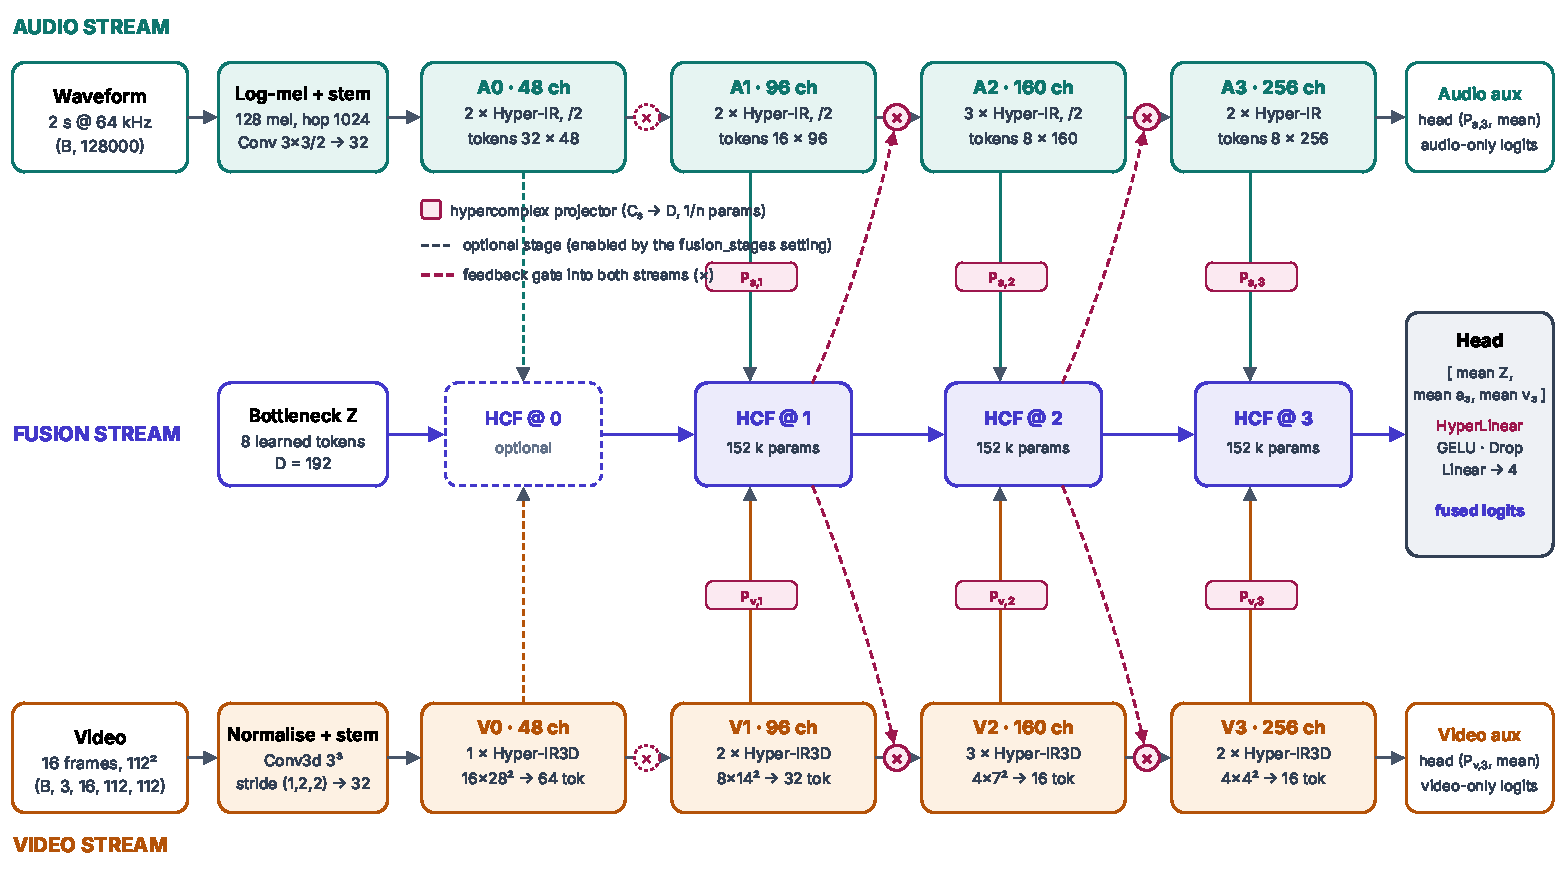
\includegraphics[width=\textwidth]{figures/arch_overview.pdf}
  \caption{HyperAVNet (default configuration: quaternion algebra, fusion stages $\mathcal{S}=\{1,2,3\}$,
  feedback enabled). Stage tokens of the audio and video backbones are projected by hypercomplex
  projectors $P_{a,s}$ and $P_{v,s}$ into a $D$-dimensional fusion space, where HCF blocks update the
  bottleneck tokens $\mathbf{Z}$. After each fused stage $s<S-1$, a zero-initialised gate ($\times$)
  modulates both streams. The classifier reads the pooled bottleneck and the pooled last-stage
  tokens; auxiliary heads supervise each modality on its own. Token shapes are for one 2\,s clip and
  $16\times112^{2}$ frames.}
  \label{fig:overview}
\end{figure*}

\subsection{Hypercomplex layers}
\label{sec:hyper}
Let $\mathbb{A}_n$ be a hypercomplex algebra of dimension $n\in\{2,4,8,16\}$ (complex numbers,
quaternions, octonions, sedenions, obtained by the Cayley--Dickson construction), with basis
$\{e_0,\dots,e_{n-1}\}$ and multiplication table
\begin{equation}
  e_i\,e_j = \sigma_{ij}\, e_{\pi(i,j)},
  \label{eq:table}
\end{equation}
with signs $\sigma_{ij}\in\{-1,+1\}$ and indices $\pi(i,j)\in\{0,\dots,n-1\}$.
A feature vector $\mathbf{x}\in\mathbb{R}^{d_{\mathrm{in}}}$ is split into $n$ components,
$\mathbf{x}=[\mathbf{x}_0;\dots;\mathbf{x}_{n-1}]$ with $\mathbf{x}_j\in\mathbb{R}^{d_{\mathrm{in}}/n}$,
i.e.\ it is read as $\sum_j \mathbf{x}_j e_j$. A hypercomplex weight
$\mathbf{W}=\sum_{k}\mathbf{W}_k e_k$ with real blocks $\mathbf{W}_k\in\mathbb{R}^{(d_{\mathrm{out}}/n)\times(d_{\mathrm{in}}/n)}$
acts on it by the algebra product, which in matrix form is
\begin{equation}
\begin{gathered}
  \mathbf{y}_i = \sum_{j=0}^{n-1} s_{ij}\,\mathbf{W}_{c(i,j)}\,\mathbf{x}_j + \mathbf{b}_i,\\
  \mathbf{K}(\mathbf{W}) = \big[\, s_{ij}\,\mathbf{W}_{c(i,j)} \,\big]_{i,j=0}^{n-1}\in\mathbb{R}^{d_{\mathrm{out}}\times d_{\mathrm{in}}},
\end{gathered}
  \label{eq:hlinear}
\end{equation}
where the block index $c(i,j)$ and sign $s_{ij}$ follow from Eq.~\eqref{eq:table}. For quaternions the
kernel takes the familiar Hamilton form (Fig.~\ref{fig:hamilton}),
\begin{equation}
  \mathbf{K} = \begin{bmatrix}
   \mathbf{W}_0 & \mathbf{W}_1 & \mathbf{W}_2 & \mathbf{W}_3\\
  -\mathbf{W}_1 & \mathbf{W}_0 & \mathbf{W}_3 & -\mathbf{W}_2\\
  -\mathbf{W}_2 & -\mathbf{W}_3 & \mathbf{W}_0 & \mathbf{W}_1\\
  -\mathbf{W}_3 & \mathbf{W}_2 & -\mathbf{W}_1 & \mathbf{W}_0
  \end{bmatrix}.
  \label{eq:hamilton}
\end{equation}
Every output component is thus a signed combination of \emph{every} input component through one
shared set of $n$ blocks, so the layer has
\begin{equation}
  |\theta_{\mathrm{hyper}}| = \tfrac{1}{n}\,d_{\mathrm{in}}d_{\mathrm{out}} + d_{\mathrm{out}}
  \;\;\text{vs.}\;\;
  |\theta_{\mathrm{real}}| = d_{\mathrm{in}}d_{\mathrm{out}} + d_{\mathrm{out}}
  \label{eq:params}
\end{equation}
parameters. A hypercomplex convolution applies the same block structure to the kernel tensor, with
$\mathbf{W}_k\in\mathbb{R}^{(C_{\mathrm{out}}/n)\times(C_{\mathrm{in}}/n)\times k_1\times\dots}$.
Weights are initialised in polar form: a modulus drawn from a $\chi$ distribution with $n$ degrees of
freedom (scaled by the Glorot variance), a uniform phase, and a unit-norm imaginary direction
\cite{bojesomo2024hypercomplex}. We write $\mathcal{H}_n(\cdot)$ for a hypercomplex linear or
convolutional layer. With $n=1$ it reduces to the real layer, which gives a matched real-valued
ablation with an identical code path.

\paragraph{Deployment.} Building $\mathbf{K}$ in Eq.~\eqref{eq:hlinear} at every forward pass
is only needed while training. After training, every $\mathcal{H}_n$ is \emph{reparameterised} into a
dense layer with weight $\mathbf{K}(\mathbf{W})$. The outputs are identical, and the run-time
overhead of kernel assembly disappears. The hypercomplex structure therefore reduces the number of
stored and optimised parameters (and the model's memory and transmission size) by up to $n\times$,
but \emph{not} the multiply--accumulate count, because $\mathbf{K}$ is dense.

\begin{figure}[t]
  \centering
  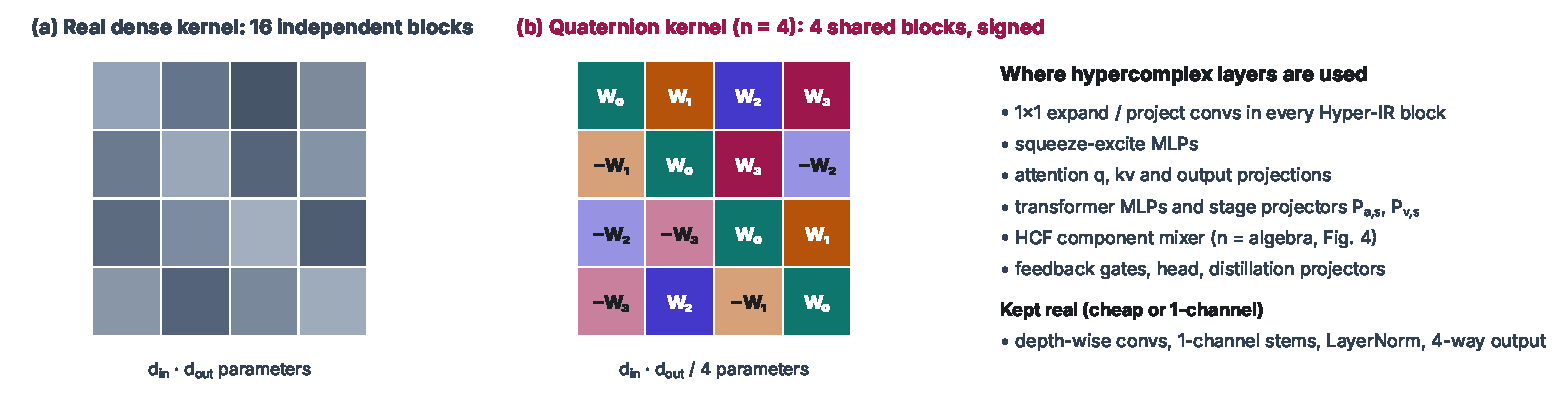
\includegraphics[width=\columnwidth]{figures/hamilton.pdf}
  \caption{Hamilton-product weight sharing. (a) A real kernel has $n^{2}$ independent blocks.
  (b) A quaternion kernel ($n=4$) re-uses four blocks with fixed signs (Eq.~\eqref{eq:hamilton}),
  which cuts the parameter count by $4\times$.}
  \label{fig:hamilton}
\end{figure}

\subsection{Hypercomplex backbones and stage tokens}
\label{sec:backbones}
\paragraph{Hyper-IR block.} Both backbones stack hypercomplex inverted-residual blocks
(Fig.~\ref{fig:hyperir}). For an input $\mathbf{h}\in\mathbb{R}^{C\times\Omega}$ ($\Omega$ is the 2-D
time--frequency grid for audio and the 3-D space--time grid for video) and expansion ratio $r=4$:
\begin{equation}
\begin{aligned}
  \mathbf{u} &= \operatorname{SiLU}\big(\operatorname{BN}(\mathcal{H}_n^{1\times1}(\mathbf{h}))\big)\in\mathbb{R}^{rC\times\Omega},\\
  \mathbf{v} &= \operatorname{SiLU}\big(\operatorname{BN}(\operatorname{DWConv}_{3}(\mathbf{u}))\big),\\
  \mathbf{w} &= \mathbf{v}\odot\sigma\big(\mathcal{H}_n(\operatorname{SiLU}(\mathcal{H}_n(\operatorname{GAP}(\mathbf{v}))))\big),\\
  \mathbf{h}' &= \mathbf{h} + \operatorname{DropPath}\big(\operatorname{BN}(\mathcal{H}_n^{1\times1}(\mathbf{w}))\big).
\end{aligned}
  \label{eq:hyperir}
\end{equation}
The two point-wise convolutions hold almost all of a block's parameters, so they are hypercomplex. The
depth-wise convolution stays real; it accounts for about 1\% of the parameters. The residual is used
when the shape is preserved.

\paragraph{Audio stream.} The waveform is converted to a log-mel spectrogram with the U-FFIA settings
(Hann window 2048, hop 1024, 128 mel bins at 64\,kHz, so a 2\,s clip gives $128\times126$),
normalised per mel bin by batch normalisation and augmented with SpecAugment during training. A
$3{\times}3$ stride-2 stem is followed by four Hyper-IR stages $s=0,\dots,3$ with widths
$(48,96,160,256)$ and depths $(2,2,3,2)$. A stage map $\mathbf{h}^{a}_{s}\in\mathbb{R}^{C_s\times T_s\times F_s}$
becomes time tokens by pooling over frequency:
\begin{equation}
  \mathbf{a}_s = \big[\operatorname{mean}_{F}(\mathbf{h}^{a}_s) + \operatorname{max}_{F}(\mathbf{h}^{a}_s)\big]^{\top}\in\mathbb{R}^{T_s\times C_s}.
  \label{eq:audiotokens}
\end{equation}
The max term keeps the short impulsive transients of feeding (chewing, tail slaps).

\paragraph{Video stream.} The frames are normalised and passed through a $3{\times}3{\times}3$ stem
(spatial stride 2) and four 3-D Hyper-IR stages of the same widths, with depths $(1,2,3,2)$ and
strides $(1,2,2)$, $(2,2,2)$, $(2,2,2)$, $(1,2,2)$. A stage map
$\mathbf{h}^{v}_{s}\in\mathbb{R}^{C_s\times T_s\times H_s\times W_s}$ is pooled to a $2\times2$ spatial grid
per time step, $\mathbf{v}_s\in\mathbb{R}^{4T_s\times C_s}$. This keeps coarse location (where the fish
aggregate) at a small token count.

\begin{figure}[t]
  \centering
  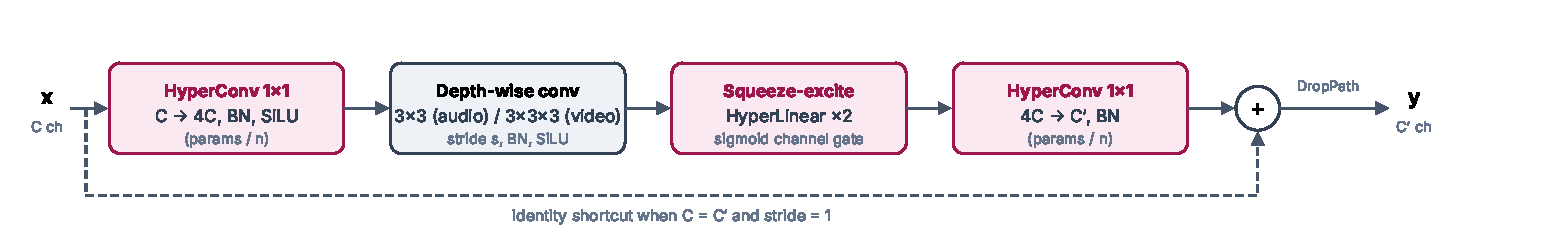
\includegraphics[width=\columnwidth]{figures/hyper_ir.pdf}
  \caption{Hypercomplex inverted-residual (Hyper-IR) block, Eq.~\eqref{eq:hyperir}. Hypercomplex
  layers are shaded; the depth-wise convolution is real.}
  \label{fig:hyperir}
\end{figure}

\paragraph{Pretrained backbones.} Any pretrained network can replace a student backbone if it exposes
four stages in the same token format. We use this for the teachers and for the teacher ablation
(Sec.~\ref{sec:setup}): PANNs CNN10/CNN14~\cite{kong2020panns}, EfficientAT~\cite{schmid2023efficientat},
AST~\cite{gong2021ast}, S3D~\cite{xie2018s3d}, X3D~\cite{feichtenhofer2020x3d},
MoViNet~\cite{kondratyuk2021movinets} and VideoMAE~\cite{tong2022videomae}. Their intermediate layers
supply the stage tokens.

\subsection{Hypercomplex component fusion}
\label{sec:hcf}
\paragraph{Projection.} Stage tokens are mapped into a shared $D$-dimensional space by hypercomplex
projectors with a learned modality embedding:
\begin{equation}
  \mathbf{A}_s = \operatorname{LN}\!\big(\mathcal{H}_n(\mathbf{a}_s)\big) + \mathbf{m}^{a},\qquad
  \mathbf{V}_s = \operatorname{LN}\!\big(\mathcal{H}_n(\mathbf{v}_s)\big) + \mathbf{m}^{v}.
  \label{eq:proj}
\end{equation}

\paragraph{Bottleneck state.} The fused representation lives in $N_b$ learned bottleneck tokens
$\mathbf{Z}\in\mathbb{R}^{N_b\times D}$ (we use $N_b=8$, $D=192$), shared across stages.

\paragraph{HCF block.} At a fusion stage $s$, the bottleneck first reads each modality with its own
hypercomplex cross-attention:
\begin{equation}
\begin{aligned}
  \mathbf{Z}^{a} &= \mathbf{Z} + \operatorname{XAttn}_{n}\big(\operatorname{LN}\mathbf{Z},\,\operatorname{LN}\mathbf{A}_s\big),\\
  \mathbf{Z}^{v} &= \mathbf{Z} + \operatorname{XAttn}_{n}\big(\operatorname{LN}\mathbf{Z},\,\operatorname{LN}\mathbf{V}_s\big),
\end{aligned}
  \label{eq:xattn}
\end{equation}
where $\operatorname{XAttn}_n$ is multi-head attention whose query, key, value and output projections
are hypercomplex (shown for one head of width $d_h$):
\begin{equation*}
  \operatorname{XAttn}_n(\mathbf{Q},\mathbf{C})=\mathcal{H}_n\Big(\operatorname{softmax}\Big(\tfrac{\mathcal{H}_n(\mathbf{Q})\,\mathcal{H}_n(\mathbf{C})^{\top}}{\sqrt{d_h}}\Big)\mathcal{H}_n(\mathbf{C})\Big).
\end{equation*} The shared
state, the two modality views and their interaction then form the components of one element of
$\mathbb{A}_m$:
\begin{equation}
  \mathbf{q} = \mathbf{Z}\,e_0 + \mathbf{Z}^{a}\,e_1 + \mathbf{Z}^{v}\,e_2 + \big(\hat{\mathbf{Z}}^{a}\odot\hat{\mathbf{Z}}^{v}\big)\,e_3,
  \label{eq:components}
\end{equation}
for $m=4$,
with $\hat{\cdot}=\operatorname{LN}(\cdot)$. The octonion variant ($m=8$) appends
$(\mathbf{Z}^{a}-\mathbf{Z}^{v})e_4$, $(\hat{\mathbf{Z}}\odot\hat{\mathbf{Z}}^{a})e_5$,
$(\hat{\mathbf{Z}}\odot\hat{\mathbf{Z}}^{v})e_6$ and
$(\hat{\mathbf{Z}}\odot\hat{\mathbf{Z}}^{a}\odot\hat{\mathbf{Z}}^{v})e_7$; the complex variant ($m=2$) uses
$(\mathbf{Z}^{a},\mathbf{Z}^{v})$. The components are mixed by a single Hamilton product, followed by a
hypercomplex MLP:
\begin{equation}
\begin{aligned}
  \mathbf{Z} &\leftarrow \mathbf{Z} + \boldsymbol{\gamma}_1\odot \mathcal{H}_m(\mathbf{q}),\\
  \mathbf{Z} &\leftarrow \mathbf{Z} + \boldsymbol{\gamma}_2\odot \operatorname{MLP}_n(\operatorname{LN}\mathbf{Z}),
\end{aligned}
  \label{eq:mix}
\end{equation}
where $\mathcal{H}_m:\mathbb{R}^{mD}\to\mathbb{R}^{D}$ is a hypercomplex linear layer of algebra
$\mathbb{A}_m$ and $\boldsymbol{\gamma}_{1,2}$ are LayerScale vectors~\cite{touvron2021cait}, initialised to
$10^{-2}$. By Eq.~\eqref{eq:hlinear}, each output component of $\mathcal{H}_m$ is a signed mixture of
the shared state, both modality views and their multiplicative agreement, all through one set of
$m$ blocks. The mixer has $D^{2}$ parameters \emph{for every} $m$, against $mD^{2}$ for a dense mixer, so
the octonion variant adds four interaction terms at no parameter cost. Unlike attention bottlenecks
that attend to the modalities one after the other~\cite{nagrani2021mbt}, HCF reads both modalities
in parallel and combines them in one algebraic product (Fig.~\ref{fig:hcf}).

\begin{figure*}[t]
  \centering
  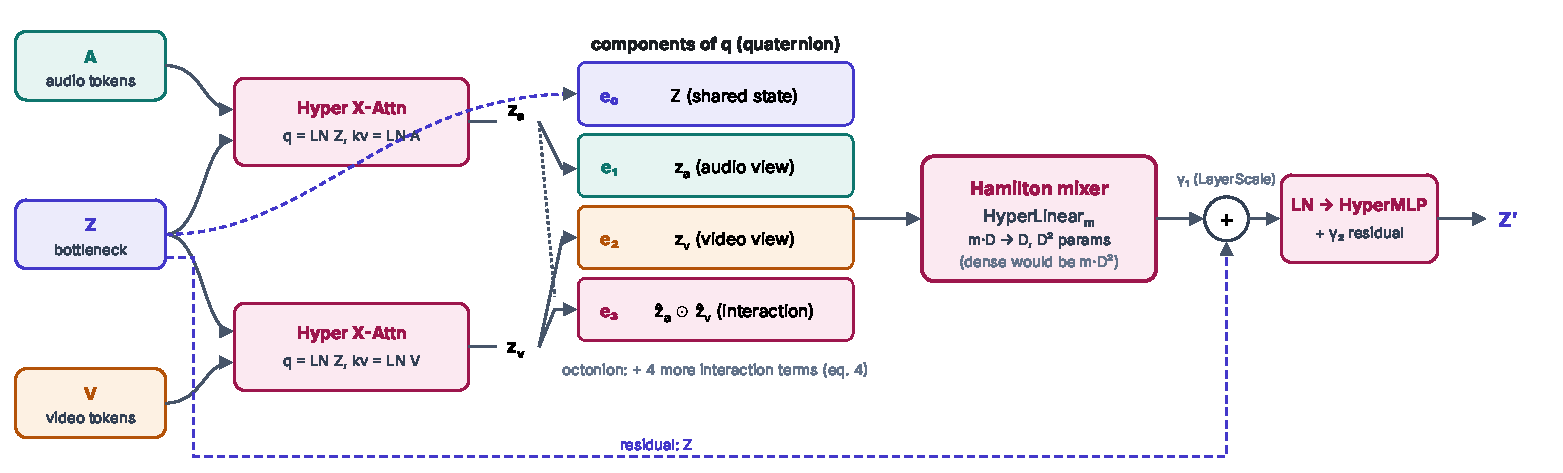
\includegraphics[width=0.9\textwidth]{figures/hcf_block.pdf}
  \caption{Hypercomplex component fusion (HCF), Eqs.~\eqref{eq:xattn}--\eqref{eq:mix}. The modality
  views and their interaction are the components of one quaternion and are mixed by a single
  Hamilton product.}
  \label{fig:hcf}
\end{figure*}

\subsection{Deep-to-early fusion schedule with cross-modal feedback}
\label{sec:schedule}
The set $\mathcal{S}\subseteq\{0,\dots,S-1\}$ selects the stages at which an HCF block is attached:
\begin{equation}
  \mathbf{Z}^{(s+1)} = \begin{cases}\operatorname{HCF}_s\big(\mathbf{Z}^{(s)},\mathbf{A}_s,\mathbf{V}_s\big), & s\in\mathcal{S},\\ \mathbf{Z}^{(s)}, & \text{otherwise,}\end{cases}
  \label{eq:schedule}
\end{equation}
with $\mathbf{Z}^{(0)}=\mathbf{Z}_{\mathrm{init}}$ the learned bottleneck tokens.
Varying $\mathcal{S}$ from $\{S-1\}$ (late fusion) through $\{S-2,S-1\}$ and so on to $\{0,\dots,S-1\}$
gives a controlled \emph{deep-to-early} study of where audio--visual fusion helps. Because the student
backbones are executed stage by stage, the fused state is also fed back into both streams after each
fused stage $s<S-1$:
\begin{equation}
  \mathbf{h}^{m}_s \leftarrow \mathbf{h}^{m}_s\odot\big(1+\tanh(\mathcal{G}^{m}_s\,\bar{\mathbf{z}}^{(s+1)})\big),\quad m\in\{a,v\},
  \label{eq:feedback}
\end{equation}
where $\bar{\mathbf{z}}=\operatorname{mean}_{N_b}(\mathbf{Z})$, the gates
$\mathcal{G}^{m}_s$ are hypercomplex linear maps $\mathbb{R}^{D}\to\mathbb{R}^{C_s}$, and the
product broadcasts over $\Omega$. The gates are \emph{initialised to zero}, so training starts exactly
at the feedback-free model. The network then learns how strongly each modality should condition the
other's later features. This is genuine early fusion, as opposed to fusing independently computed
features.

\subsection{Prediction heads and modality dropout}
\label{sec:heads}
With $\bar{\mathbf{z}}=\operatorname{mean}(\operatorname{LN}\mathbf{Z}^{(S)})$,
$\bar{\mathbf{a}}=\operatorname{mean}(\operatorname{LN}\mathbf{A}_{S-1})$ and
$\bar{\mathbf{v}}=\operatorname{mean}(\operatorname{LN}\mathbf{V}_{S-1})$, the fused and auxiliary logits are
\begin{equation}
\begin{gathered}
  \boldsymbol{\ell} = \mathbf{W}_o\,\operatorname{GELU}\big(\mathcal{H}_n[\bar{\mathbf{z}};\,\mu_a\bar{\mathbf{a}};\,\mu_v\bar{\mathbf{v}}]\big),\\
  \boldsymbol{\ell}^{a} = \mathbf{W}_a\bar{\mathbf{a}},\qquad \boldsymbol{\ell}^{v} = \mathbf{W}_v\bar{\mathbf{v}}.
\end{gathered}
  \label{eq:heads}
\end{equation}
Here $\mu_a,\mu_v\in\{0,1\}$ are per-sample modality masks. During training,
$(\mu_a,\mu_v)=(0,1)$ with probability $p$, $(1,0)$ with probability $p$, and $(1,1)$ otherwise. In the
notation of~\cite{cui2024uffia}, $p_{av}=1-2p$ and $p_a=p_v=p$. The same mask multiplies every fusion
input $\mathbf{A}_s,\mathbf{V}_s$, so a dropped modality is absent everywhere. The auxiliary heads always see
their own modality, which keeps both branches trained regardless of $p$. At test time, forcing
$\mu_a=0$ or $\mu_v=0$ evaluates the model with a missing modality.

\subsection{Training objective and multi-level distillation}
\label{sec:objective}
The supervised loss combines label-smoothed cross-entropy on the fused logits with the two
auxiliary terms:
\begin{equation}
  \mathcal{L}_{\mathrm{sup}} = \operatorname{CE}_{\epsilon}(\boldsymbol{\ell},y)
   + \tfrac{\lambda_{\mathrm{aux}}}{2}\!\!\sum_{m\in\{a,v\}}\!\!\operatorname{CE}_{\epsilon}(\boldsymbol{\ell}^{m},y).
  \label{eq:sup}
\end{equation}
A frozen teacher $g$ with the same output structure (pretrained backbones and HCF fusion) provides
three further signals. At the \emph{logit level}, with temperature $\tau$:
\begin{equation}
  \mathcal{L}_{\mathrm{KD}} = \tau^{2}\,\mathrm{KL}\big(\boldsymbol{\ell}^{g}\,\|\,\boldsymbol{\ell}\big)_{\tau}
   + \tfrac{\lambda_{u}\tau^{2}}{2}\!\!\sum_{m\in\{a,v\}}\!\!\mathrm{KL}\big(\boldsymbol{\ell}^{g,m}\,\|\,\boldsymbol{\ell}^{m}\big)_{\tau},
  \label{eq:kd}
\end{equation}
with $\mathrm{KL}(\mathbf{u}\,\|\,\mathbf{w})_{\tau}=\mathrm{KL}\big(\operatorname{softmax}(\mathbf{u}/\tau)\,\|\,\operatorname{softmax}(\mathbf{w}/\tau)\big)$,
which distils each unimodal head from its counterpart in the teacher. U-FFIA's variant~\cite{cui2024uffia}
softens only the teacher, $\mathrm{KL}(\operatorname{softmax}(\boldsymbol{\ell}^{g}/\tau)\,\|\,\operatorname{softmax}(\boldsymbol{\ell}))$,
and is evaluated as an ablation. At the \emph{embedding level}, small hypercomplex projectors
$\mathcal{P}_k$ align the student's pooled embeddings with the teacher's:
\begin{equation}
  \mathcal{L}_{\mathrm{feat}} = \tfrac{1}{3}\!\!\sum_{k\in\{\bar{\mathbf{z}},\bar{\mathbf{a}},\bar{\mathbf{v}}\}}\!\!
  \big(1-\cos(\mathcal{P}_k(k),\,k^{g})\big).
  \label{eq:feat}
\end{equation}
At the \emph{relation level}~\cite{park2019rkd}, the within-batch similarity structure of the fused
embeddings is matched:
\begin{equation}
  \mathcal{L}_{\mathrm{rel}} = \operatorname{SmoothL1}\big(\mathbf{R}(\bar{\mathbf{z}}_{1:B}),\,\mathbf{R}(\bar{\mathbf{z}}^{g}_{1:B})\big),
  \label{eq:rel}
\end{equation}
where $\mathbf{R}(\mathbf{U})_{ij}=\mathbf{u}_i^{\top}\mathbf{u}_j/(\|\mathbf{u}_i\|\|\mathbf{u}_j\|)$ is the cosine-similarity matrix of a batch of size $B$.
The full objective is
\begin{equation}
  \mathcal{L} = \mathcal{L}_{\mathrm{sup}} + \alpha\,\mathcal{L}_{\mathrm{KD}} + \beta\,\mathcal{L}_{\mathrm{feat}} + \gamma\,\mathcal{L}_{\mathrm{rel}},
  \label{eq:total}
\end{equation}
with $\epsilon=0.1$, $\lambda_{\mathrm{aux}}=0.3$, $\lambda_u=0.5$, $\tau=2$, $\alpha=0.7$, $\beta=1$ and $\gamma=0.5$.
Training proceeds in two stages: the teacher is trained with $\mathcal{L}_{\mathrm{sup}}$ and frozen, then
the student is trained with Eq.~\eqref{eq:total}.

\begin{figure*}[t]
  \centering
  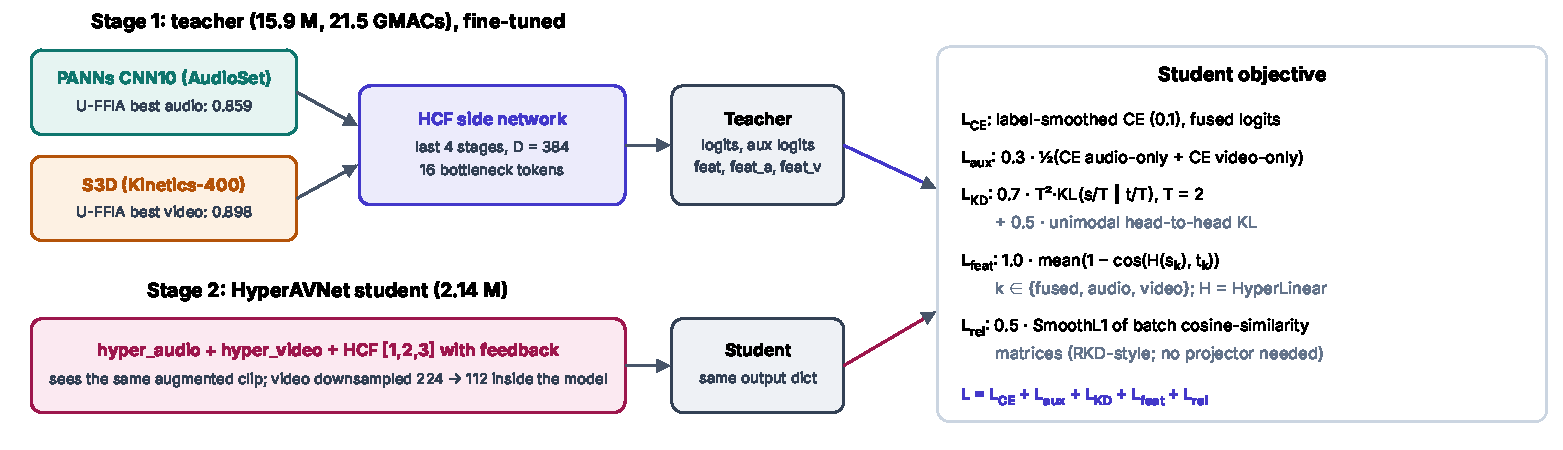
\includegraphics[width=0.92\textwidth]{figures/distillation.pdf}
  \caption{Two-stage training. A teacher built from pretrained audio and video backbones and HCF fusion
  is trained first and frozen. The HyperAVNet student is then trained with the supervised loss plus
  logit-, embedding- and relation-level distillation (Eq.~\eqref{eq:total}).}
  \label{fig:distill}
\end{figure*}

\subsection{Complexity}
\label{sec:complexity}
By Eq.~\eqref{eq:params}, every hypercomplex projection stores $1/n$ of the real parameters. Only the
stems, the depth-wise convolutions, normalisation layers and the final $4$-way classifier stay real.
For the default student ($n=4$), the network has 2.14\,M parameters against 7.88\,M for the identical
real network ($n=1$), and 1.24\,M (octonion) or 0.78\,M (sedenion) for higher algebras. Compute is
1.18\,GMACs per clip for every $n$ (16 frames at $112^{2}$ and 2\,s of audio). The added cost of a
fusion stage is about 0.17\,M parameters and under 0.02\,GMACs.
 in any paper.
%  Requires: amsmath, amssymb, bm, booktabs, graphicx, (cleveref optional).
% ============================================================================
\section{Methodology}
\label{sec:method}

\subsection{Problem formulation}
\label{sec:problem}
Each sample of AV-FFIA is a synchronised two-second clip $(\mathbf{x}^{a}, \mathbf{X}^{v})$, where
$\mathbf{x}^{a}\in\mathbb{R}^{L}$ is the hydrophone waveform ($L = 2f_s$, $f_s = 64$\,kHz) and
$\mathbf{X}^{v}\in[0,1]^{3\times T\times H\times W}$ holds $T$ RGB frames sampled uniformly from the
overhead camera. The label $y\in\mathcal{Y}=\{\textsc{None},\textsc{Weak},\textsc{Medium},\textsc{Strong}\}$
is the feeding intensity. We learn $f_{\theta}:(\mathbf{x}^{a},\mathbf{X}^{v})\mapsto\mathbf{p}\in\Delta^{|\mathcal{Y}|-1}$ with
two goals that pull in opposite directions: high accuracy, robust to the acoustic and visual
corruptions typical of aquaculture (bubbles, pumps, low light, reflections), and a small
parameter and compute budget for on-site deployment.

HyperAVNet (Fig.~\ref{fig:overview}) has four parts. Two hypercomplex backbones map each modality to a
hierarchy of \emph{stage tokens} (Sec.~\ref{sec:backbones}). A set of shared \emph{bottleneck tokens}
is updated by hypercomplex component fusion (HCF) blocks attached at a configurable subset of
stages, with zero-initialised cross-modal feedback into both streams (Secs.~\ref{sec:hcf},~\ref{sec:schedule}).
Fused and unimodal heads produce the predictions (Sec.~\ref{sec:heads}). The model is trained with a
multi-level distillation objective from a pretrained audio-visual teacher (Sec.~\ref{sec:objective}).

\begin{figure*}[t]
  \centering
  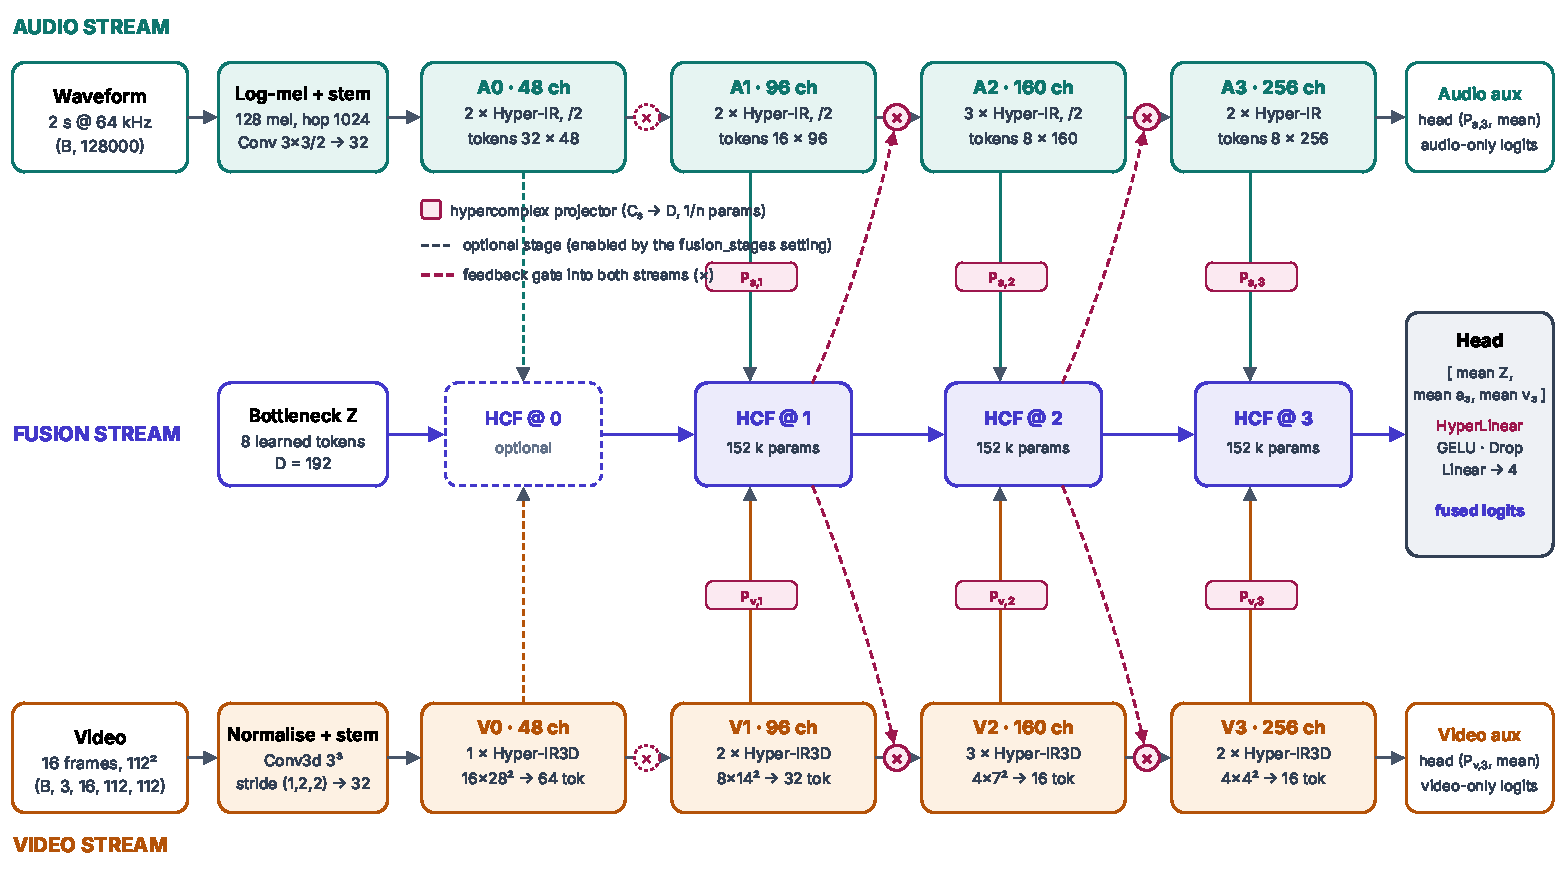
\includegraphics[width=\textwidth]{figures/arch_overview.pdf}
  \caption{HyperAVNet (default configuration: quaternion algebra, fusion stages $\mathcal{S}=\{1,2,3\}$,
  feedback enabled). Stage tokens of the audio and video backbones are projected by hypercomplex
  projectors $P_{a,s}$ and $P_{v,s}$ into a $D$-dimensional fusion space, where HCF blocks update the
  bottleneck tokens $\mathbf{Z}$. After each fused stage $s<S-1$, a zero-initialised gate ($\times$)
  modulates both streams. The classifier reads the pooled bottleneck and the pooled last-stage
  tokens; auxiliary heads supervise each modality on its own. Token shapes are for one 2\,s clip and
  $16\times112^{2}$ frames.}
  \label{fig:overview}
\end{figure*}

\subsection{Hypercomplex layers}
\label{sec:hyper}
Let $\mathbb{A}_n$ be a hypercomplex algebra of dimension $n\in\{2,4,8,16\}$ (complex numbers,
quaternions, octonions, sedenions, obtained by the Cayley--Dickson construction), with basis
$\{e_0,\dots,e_{n-1}\}$ and multiplication table
\begin{equation}
  e_i\,e_j = \sigma_{ij}\, e_{\pi(i,j)},
  \label{eq:table}
\end{equation}
with signs $\sigma_{ij}\in\{-1,+1\}$ and indices $\pi(i,j)\in\{0,\dots,n-1\}$.
A feature vector $\mathbf{x}\in\mathbb{R}^{d_{\mathrm{in}}}$ is split into $n$ components,
$\mathbf{x}=[\mathbf{x}_0;\dots;\mathbf{x}_{n-1}]$ with $\mathbf{x}_j\in\mathbb{R}^{d_{\mathrm{in}}/n}$,
i.e.\ it is read as $\sum_j \mathbf{x}_j e_j$. A hypercomplex weight
$\mathbf{W}=\sum_{k}\mathbf{W}_k e_k$ with real blocks $\mathbf{W}_k\in\mathbb{R}^{(d_{\mathrm{out}}/n)\times(d_{\mathrm{in}}/n)}$
acts on it by the algebra product, which in matrix form is
\begin{equation}
\begin{gathered}
  \mathbf{y}_i = \sum_{j=0}^{n-1} s_{ij}\,\mathbf{W}_{c(i,j)}\,\mathbf{x}_j + \mathbf{b}_i,\\
  \mathbf{K}(\mathbf{W}) = \big[\, s_{ij}\,\mathbf{W}_{c(i,j)} \,\big]_{i,j=0}^{n-1}\in\mathbb{R}^{d_{\mathrm{out}}\times d_{\mathrm{in}}},
\end{gathered}
  \label{eq:hlinear}
\end{equation}
where the block index $c(i,j)$ and sign $s_{ij}$ follow from Eq.~\eqref{eq:table}. For quaternions the
kernel takes the familiar Hamilton form (Fig.~\ref{fig:hamilton}),
\begin{equation}
  \mathbf{K} = \begin{bmatrix}
   \mathbf{W}_0 & \mathbf{W}_1 & \mathbf{W}_2 & \mathbf{W}_3\\
  -\mathbf{W}_1 & \mathbf{W}_0 & \mathbf{W}_3 & -\mathbf{W}_2\\
  -\mathbf{W}_2 & -\mathbf{W}_3 & \mathbf{W}_0 & \mathbf{W}_1\\
  -\mathbf{W}_3 & \mathbf{W}_2 & -\mathbf{W}_1 & \mathbf{W}_0
  \end{bmatrix}.
  \label{eq:hamilton}
\end{equation}
Every output component is thus a signed combination of \emph{every} input component through one
shared set of $n$ blocks, so the layer has
\begin{equation}
  |\theta_{\mathrm{hyper}}| = \tfrac{1}{n}\,d_{\mathrm{in}}d_{\mathrm{out}} + d_{\mathrm{out}}
  \;\;\text{vs.}\;\;
  |\theta_{\mathrm{real}}| = d_{\mathrm{in}}d_{\mathrm{out}} + d_{\mathrm{out}}
  \label{eq:params}
\end{equation}
parameters. A hypercomplex convolution applies the same block structure to the kernel tensor, with
$\mathbf{W}_k\in\mathbb{R}^{(C_{\mathrm{out}}/n)\times(C_{\mathrm{in}}/n)\times k_1\times\dots}$.
Weights are initialised in polar form: a modulus drawn from a $\chi$ distribution with $n$ degrees of
freedom (scaled by the Glorot variance), a uniform phase, and a unit-norm imaginary direction
\cite{bojesomo2024hypercomplex}. We write $\mathcal{H}_n(\cdot)$ for a hypercomplex linear or
convolutional layer. With $n=1$ it reduces to the real layer, which gives a matched real-valued
ablation with an identical code path.

\paragraph{Deployment.} Building $\mathbf{K}$ in Eq.~\eqref{eq:hlinear} at every forward pass
is only needed while training. After training, every $\mathcal{H}_n$ is \emph{reparameterised} into a
dense layer with weight $\mathbf{K}(\mathbf{W})$. The outputs are identical, and the run-time
overhead of kernel assembly disappears. The hypercomplex structure therefore reduces the number of
stored and optimised parameters (and the model's memory and transmission size) by up to $n\times$,
but \emph{not} the multiply--accumulate count, because $\mathbf{K}$ is dense.

\begin{figure}[t]
  \centering
  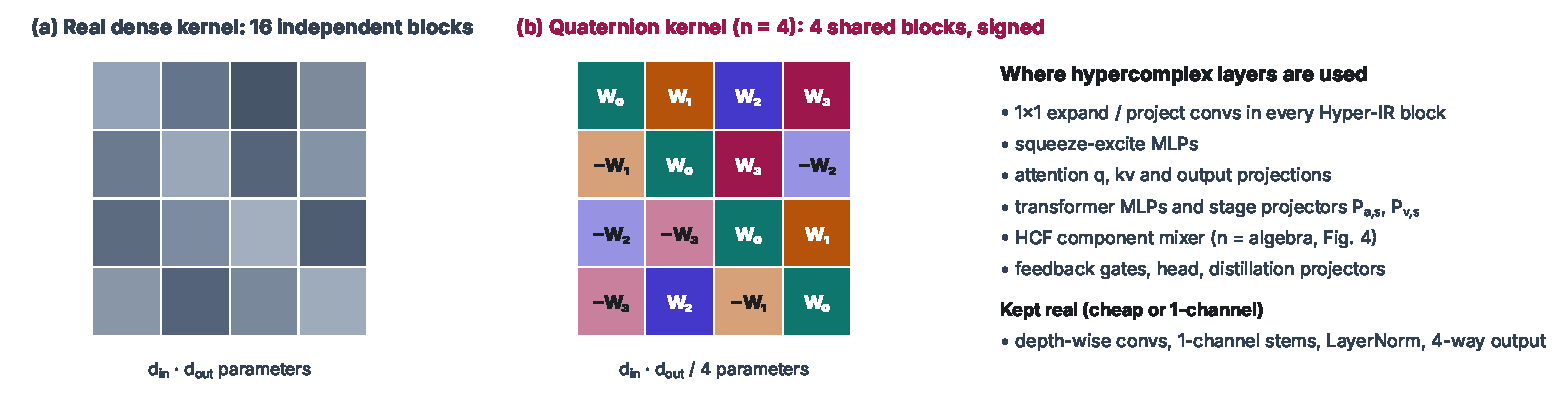
\includegraphics[width=\columnwidth]{figures/hamilton.pdf}
  \caption{Hamilton-product weight sharing. (a) A real kernel has $n^{2}$ independent blocks.
  (b) A quaternion kernel ($n=4$) re-uses four blocks with fixed signs (Eq.~\eqref{eq:hamilton}),
  which cuts the parameter count by $4\times$.}
  \label{fig:hamilton}
\end{figure}

\subsection{Hypercomplex backbones and stage tokens}
\label{sec:backbones}
\paragraph{Hyper-IR block.} Both backbones stack hypercomplex inverted-residual blocks
(Fig.~\ref{fig:hyperir}). For an input $\mathbf{h}\in\mathbb{R}^{C\times\Omega}$ ($\Omega$ is the 2-D
time--frequency grid for audio and the 3-D space--time grid for video) and expansion ratio $r=4$:
\begin{equation}
\begin{aligned}
  \mathbf{u} &= \operatorname{SiLU}\big(\operatorname{BN}(\mathcal{H}_n^{1\times1}(\mathbf{h}))\big)\in\mathbb{R}^{rC\times\Omega},\\
  \mathbf{v} &= \operatorname{SiLU}\big(\operatorname{BN}(\operatorname{DWConv}_{3}(\mathbf{u}))\big),\\
  \mathbf{w} &= \mathbf{v}\odot\sigma\big(\mathcal{H}_n(\operatorname{SiLU}(\mathcal{H}_n(\operatorname{GAP}(\mathbf{v}))))\big),\\
  \mathbf{h}' &= \mathbf{h} + \operatorname{DropPath}\big(\operatorname{BN}(\mathcal{H}_n^{1\times1}(\mathbf{w}))\big).
\end{aligned}
  \label{eq:hyperir}
\end{equation}
The two point-wise convolutions hold almost all of a block's parameters, so they are hypercomplex. The
depth-wise convolution stays real; it accounts for about 1\% of the parameters. The residual is used
when the shape is preserved.

\paragraph{Audio stream.} The waveform is converted to a log-mel spectrogram with the U-FFIA settings
(Hann window 2048, hop 1024, 128 mel bins at 64\,kHz, so a 2\,s clip gives $128\times126$),
normalised per mel bin by batch normalisation and augmented with SpecAugment during training. A
$3{\times}3$ stride-2 stem is followed by four Hyper-IR stages $s=0,\dots,3$ with widths
$(48,96,160,256)$ and depths $(2,2,3,2)$. A stage map $\mathbf{h}^{a}_{s}\in\mathbb{R}^{C_s\times T_s\times F_s}$
becomes time tokens by pooling over frequency:
\begin{equation}
  \mathbf{a}_s = \big[\operatorname{mean}_{F}(\mathbf{h}^{a}_s) + \operatorname{max}_{F}(\mathbf{h}^{a}_s)\big]^{\top}\in\mathbb{R}^{T_s\times C_s}.
  \label{eq:audiotokens}
\end{equation}
The max term keeps the short impulsive transients of feeding (chewing, tail slaps).

\paragraph{Video stream.} The frames are normalised and passed through a $3{\times}3{\times}3$ stem
(spatial stride 2) and four 3-D Hyper-IR stages of the same widths, with depths $(1,2,3,2)$ and
strides $(1,2,2)$, $(2,2,2)$, $(2,2,2)$, $(1,2,2)$. A stage map
$\mathbf{h}^{v}_{s}\in\mathbb{R}^{C_s\times T_s\times H_s\times W_s}$ is pooled to a $2\times2$ spatial grid
per time step, $\mathbf{v}_s\in\mathbb{R}^{4T_s\times C_s}$. This keeps coarse location (where the fish
aggregate) at a small token count.

\begin{figure}[t]
  \centering
  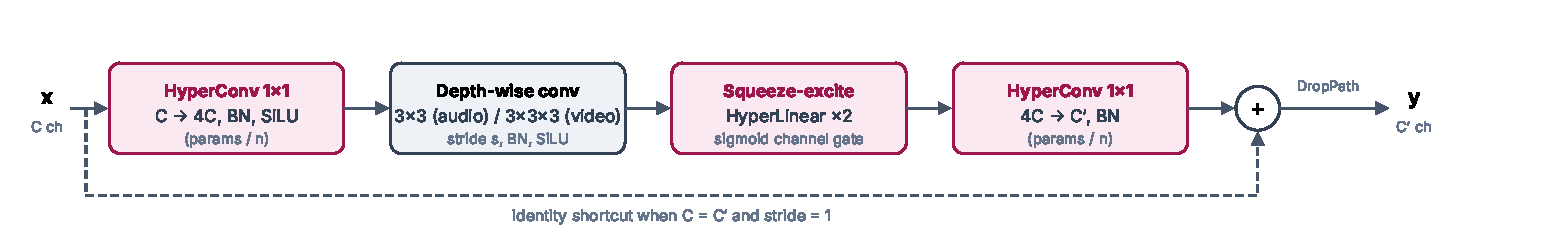
\includegraphics[width=\columnwidth]{figures/hyper_ir.pdf}
  \caption{Hypercomplex inverted-residual (Hyper-IR) block, Eq.~\eqref{eq:hyperir}. Hypercomplex
  layers are shaded; the depth-wise convolution is real.}
  \label{fig:hyperir}
\end{figure}

\paragraph{Pretrained backbones.} Any pretrained network can replace a student backbone if it exposes
four stages in the same token format. We use this for the teachers and for the teacher ablation
(Sec.~\ref{sec:setup}): PANNs CNN10/CNN14~\cite{kong2020panns}, EfficientAT~\cite{schmid2023efficientat},
AST~\cite{gong2021ast}, S3D~\cite{xie2018s3d}, X3D~\cite{feichtenhofer2020x3d},
MoViNet~\cite{kondratyuk2021movinets} and VideoMAE~\cite{tong2022videomae}. Their intermediate layers
supply the stage tokens.

\subsection{Hypercomplex component fusion}
\label{sec:hcf}
\paragraph{Projection.} Stage tokens are mapped into a shared $D$-dimensional space by hypercomplex
projectors with a learned modality embedding:
\begin{equation}
  \mathbf{A}_s = \operatorname{LN}\!\big(\mathcal{H}_n(\mathbf{a}_s)\big) + \mathbf{m}^{a},\qquad
  \mathbf{V}_s = \operatorname{LN}\!\big(\mathcal{H}_n(\mathbf{v}_s)\big) + \mathbf{m}^{v}.
  \label{eq:proj}
\end{equation}

\paragraph{Bottleneck state.} The fused representation lives in $N_b$ learned bottleneck tokens
$\mathbf{Z}\in\mathbb{R}^{N_b\times D}$ (we use $N_b=8$, $D=192$), shared across stages.

\paragraph{HCF block.} At a fusion stage $s$, the bottleneck first reads each modality with its own
hypercomplex cross-attention:
\begin{equation}
\begin{aligned}
  \mathbf{Z}^{a} &= \mathbf{Z} + \operatorname{XAttn}_{n}\big(\operatorname{LN}\mathbf{Z},\,\operatorname{LN}\mathbf{A}_s\big),\\
  \mathbf{Z}^{v} &= \mathbf{Z} + \operatorname{XAttn}_{n}\big(\operatorname{LN}\mathbf{Z},\,\operatorname{LN}\mathbf{V}_s\big),
\end{aligned}
  \label{eq:xattn}
\end{equation}
where $\operatorname{XAttn}_n$ is multi-head attention whose query, key, value and output projections
are hypercomplex (shown for one head of width $d_h$):
\begin{equation*}
  \operatorname{XAttn}_n(\mathbf{Q},\mathbf{C})=\mathcal{H}_n\Big(\operatorname{softmax}\Big(\tfrac{\mathcal{H}_n(\mathbf{Q})\,\mathcal{H}_n(\mathbf{C})^{\top}}{\sqrt{d_h}}\Big)\mathcal{H}_n(\mathbf{C})\Big).
\end{equation*} The shared
state, the two modality views and their interaction then form the components of one element of
$\mathbb{A}_m$:
\begin{equation}
  \mathbf{q} = \mathbf{Z}\,e_0 + \mathbf{Z}^{a}\,e_1 + \mathbf{Z}^{v}\,e_2 + \big(\hat{\mathbf{Z}}^{a}\odot\hat{\mathbf{Z}}^{v}\big)\,e_3,
  \label{eq:components}
\end{equation}
for $m=4$,
with $\hat{\cdot}=\operatorname{LN}(\cdot)$. The octonion variant ($m=8$) appends
$(\mathbf{Z}^{a}-\mathbf{Z}^{v})e_4$, $(\hat{\mathbf{Z}}\odot\hat{\mathbf{Z}}^{a})e_5$,
$(\hat{\mathbf{Z}}\odot\hat{\mathbf{Z}}^{v})e_6$ and
$(\hat{\mathbf{Z}}\odot\hat{\mathbf{Z}}^{a}\odot\hat{\mathbf{Z}}^{v})e_7$; the complex variant ($m=2$) uses
$(\mathbf{Z}^{a},\mathbf{Z}^{v})$. The components are mixed by a single Hamilton product, followed by a
hypercomplex MLP:
\begin{equation}
\begin{aligned}
  \mathbf{Z} &\leftarrow \mathbf{Z} + \boldsymbol{\gamma}_1\odot \mathcal{H}_m(\mathbf{q}),\\
  \mathbf{Z} &\leftarrow \mathbf{Z} + \boldsymbol{\gamma}_2\odot \operatorname{MLP}_n(\operatorname{LN}\mathbf{Z}),
\end{aligned}
  \label{eq:mix}
\end{equation}
where $\mathcal{H}_m:\mathbb{R}^{mD}\to\mathbb{R}^{D}$ is a hypercomplex linear layer of algebra
$\mathbb{A}_m$ and $\boldsymbol{\gamma}_{1,2}$ are LayerScale vectors~\cite{touvron2021cait}, initialised to
$10^{-2}$. By Eq.~\eqref{eq:hlinear}, each output component of $\mathcal{H}_m$ is a signed mixture of
the shared state, both modality views and their multiplicative agreement, all through one set of
$m$ blocks. The mixer has $D^{2}$ parameters \emph{for every} $m$, against $mD^{2}$ for a dense mixer, so
the octonion variant adds four interaction terms at no parameter cost. Unlike attention bottlenecks
that attend to the modalities one after the other~\cite{nagrani2021mbt}, HCF reads both modalities
in parallel and combines them in one algebraic product (Fig.~\ref{fig:hcf}).

\begin{figure*}[t]
  \centering
  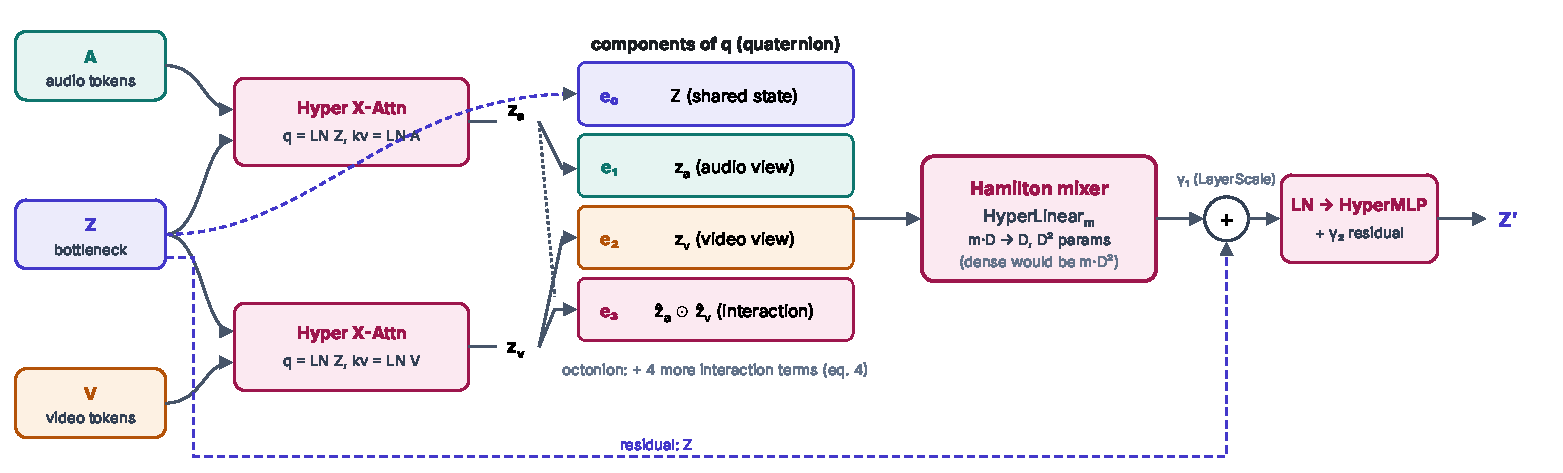
\includegraphics[width=0.9\textwidth]{figures/hcf_block.pdf}
  \caption{Hypercomplex component fusion (HCF), Eqs.~\eqref{eq:xattn}--\eqref{eq:mix}. The modality
  views and their interaction are the components of one quaternion and are mixed by a single
  Hamilton product.}
  \label{fig:hcf}
\end{figure*}

\subsection{Deep-to-early fusion schedule with cross-modal feedback}
\label{sec:schedule}
The set $\mathcal{S}\subseteq\{0,\dots,S-1\}$ selects the stages at which an HCF block is attached:
\begin{equation}
  \mathbf{Z}^{(s+1)} = \begin{cases}\operatorname{HCF}_s\big(\mathbf{Z}^{(s)},\mathbf{A}_s,\mathbf{V}_s\big), & s\in\mathcal{S},\\ \mathbf{Z}^{(s)}, & \text{otherwise,}\end{cases}
  \label{eq:schedule}
\end{equation}
with $\mathbf{Z}^{(0)}=\mathbf{Z}_{\mathrm{init}}$ the learned bottleneck tokens.
Varying $\mathcal{S}$ from $\{S-1\}$ (late fusion) through $\{S-2,S-1\}$ and so on to $\{0,\dots,S-1\}$
gives a controlled \emph{deep-to-early} study of where audio--visual fusion helps. Because the student
backbones are executed stage by stage, the fused state is also fed back into both streams after each
fused stage $s<S-1$:
\begin{equation}
  \mathbf{h}^{m}_s \leftarrow \mathbf{h}^{m}_s\odot\big(1+\tanh(\mathcal{G}^{m}_s\,\bar{\mathbf{z}}^{(s+1)})\big),\quad m\in\{a,v\},
  \label{eq:feedback}
\end{equation}
where $\bar{\mathbf{z}}=\operatorname{mean}_{N_b}(\mathbf{Z})$, the gates
$\mathcal{G}^{m}_s$ are hypercomplex linear maps $\mathbb{R}^{D}\to\mathbb{R}^{C_s}$, and the
product broadcasts over $\Omega$. The gates are \emph{initialised to zero}, so training starts exactly
at the feedback-free model. The network then learns how strongly each modality should condition the
other's later features. This is genuine early fusion, as opposed to fusing independently computed
features.

\subsection{Prediction heads and modality dropout}
\label{sec:heads}
With $\bar{\mathbf{z}}=\operatorname{mean}(\operatorname{LN}\mathbf{Z}^{(S)})$,
$\bar{\mathbf{a}}=\operatorname{mean}(\operatorname{LN}\mathbf{A}_{S-1})$ and
$\bar{\mathbf{v}}=\operatorname{mean}(\operatorname{LN}\mathbf{V}_{S-1})$, the fused and auxiliary logits are
\begin{equation}
\begin{gathered}
  \boldsymbol{\ell} = \mathbf{W}_o\,\operatorname{GELU}\big(\mathcal{H}_n[\bar{\mathbf{z}};\,\mu_a\bar{\mathbf{a}};\,\mu_v\bar{\mathbf{v}}]\big),\\
  \boldsymbol{\ell}^{a} = \mathbf{W}_a\bar{\mathbf{a}},\qquad \boldsymbol{\ell}^{v} = \mathbf{W}_v\bar{\mathbf{v}}.
\end{gathered}
  \label{eq:heads}
\end{equation}
Here $\mu_a,\mu_v\in\{0,1\}$ are per-sample modality masks. During training,
$(\mu_a,\mu_v)=(0,1)$ with probability $p$, $(1,0)$ with probability $p$, and $(1,1)$ otherwise. In the
notation of~\cite{cui2024uffia}, $p_{av}=1-2p$ and $p_a=p_v=p$. The same mask multiplies every fusion
input $\mathbf{A}_s,\mathbf{V}_s$, so a dropped modality is absent everywhere. The auxiliary heads always see
their own modality, which keeps both branches trained regardless of $p$. At test time, forcing
$\mu_a=0$ or $\mu_v=0$ evaluates the model with a missing modality.

\subsection{Training objective and multi-level distillation}
\label{sec:objective}
The supervised loss combines label-smoothed cross-entropy on the fused logits with the two
auxiliary terms:
\begin{equation}
  \mathcal{L}_{\mathrm{sup}} = \operatorname{CE}_{\epsilon}(\boldsymbol{\ell},y)
   + \tfrac{\lambda_{\mathrm{aux}}}{2}\!\!\sum_{m\in\{a,v\}}\!\!\operatorname{CE}_{\epsilon}(\boldsymbol{\ell}^{m},y).
  \label{eq:sup}
\end{equation}
A frozen teacher $g$ with the same output structure (pretrained backbones and HCF fusion) provides
three further signals. At the \emph{logit level}, with temperature $\tau$:
\begin{equation}
  \mathcal{L}_{\mathrm{KD}} = \tau^{2}\,\mathrm{KL}\big(\boldsymbol{\ell}^{g}\,\|\,\boldsymbol{\ell}\big)_{\tau}
   + \tfrac{\lambda_{u}\tau^{2}}{2}\!\!\sum_{m\in\{a,v\}}\!\!\mathrm{KL}\big(\boldsymbol{\ell}^{g,m}\,\|\,\boldsymbol{\ell}^{m}\big)_{\tau},
  \label{eq:kd}
\end{equation}
with $\mathrm{KL}(\mathbf{u}\,\|\,\mathbf{w})_{\tau}=\mathrm{KL}\big(\operatorname{softmax}(\mathbf{u}/\tau)\,\|\,\operatorname{softmax}(\mathbf{w}/\tau)\big)$,
which distils each unimodal head from its counterpart in the teacher. U-FFIA's variant~\cite{cui2024uffia}
softens only the teacher, $\mathrm{KL}(\operatorname{softmax}(\boldsymbol{\ell}^{g}/\tau)\,\|\,\operatorname{softmax}(\boldsymbol{\ell}))$,
and is evaluated as an ablation. At the \emph{embedding level}, small hypercomplex projectors
$\mathcal{P}_k$ align the student's pooled embeddings with the teacher's:
\begin{equation}
  \mathcal{L}_{\mathrm{feat}} = \tfrac{1}{3}\!\!\sum_{k\in\{\bar{\mathbf{z}},\bar{\mathbf{a}},\bar{\mathbf{v}}\}}\!\!
  \big(1-\cos(\mathcal{P}_k(k),\,k^{g})\big).
  \label{eq:feat}
\end{equation}
At the \emph{relation level}~\cite{park2019rkd}, the within-batch similarity structure of the fused
embeddings is matched:
\begin{equation}
  \mathcal{L}_{\mathrm{rel}} = \operatorname{SmoothL1}\big(\mathbf{R}(\bar{\mathbf{z}}_{1:B}),\,\mathbf{R}(\bar{\mathbf{z}}^{g}_{1:B})\big),
  \label{eq:rel}
\end{equation}
where $\mathbf{R}(\mathbf{U})_{ij}=\mathbf{u}_i^{\top}\mathbf{u}_j/(\|\mathbf{u}_i\|\|\mathbf{u}_j\|)$ is the cosine-similarity matrix of a batch of size $B$.
The full objective is
\begin{equation}
  \mathcal{L} = \mathcal{L}_{\mathrm{sup}} + \alpha\,\mathcal{L}_{\mathrm{KD}} + \beta\,\mathcal{L}_{\mathrm{feat}} + \gamma\,\mathcal{L}_{\mathrm{rel}},
  \label{eq:total}
\end{equation}
with $\epsilon=0.1$, $\lambda_{\mathrm{aux}}=0.3$, $\lambda_u=0.5$, $\tau=2$, $\alpha=0.7$, $\beta=1$ and $\gamma=0.5$.
Training proceeds in two stages: the teacher is trained with $\mathcal{L}_{\mathrm{sup}}$ and frozen, then
the student is trained with Eq.~\eqref{eq:total}.

\begin{figure*}[t]
  \centering
  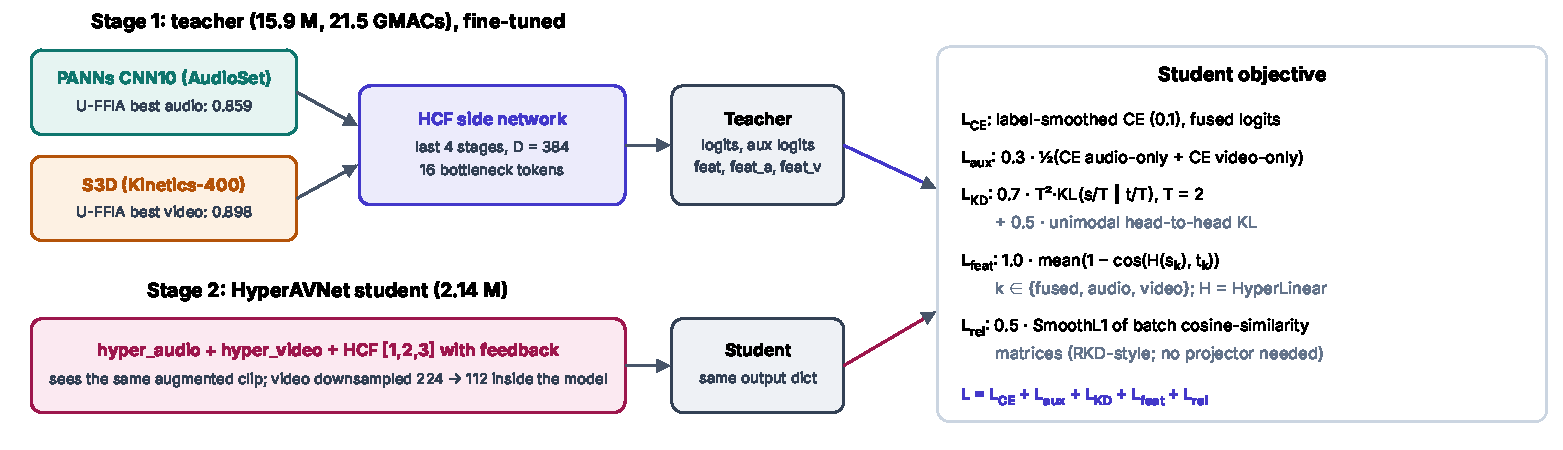
\includegraphics[width=0.92\textwidth]{figures/distillation.pdf}
  \caption{Two-stage training. A teacher built from pretrained audio and video backbones and HCF fusion
  is trained first and frozen. The HyperAVNet student is then trained with the supervised loss plus
  logit-, embedding- and relation-level distillation (Eq.~\eqref{eq:total}).}
  \label{fig:distill}
\end{figure*}

\subsection{Complexity}
\label{sec:complexity}
By Eq.~\eqref{eq:params}, every hypercomplex projection stores $1/n$ of the real parameters. Only the
stems, the depth-wise convolutions, normalisation layers and the final $4$-way classifier stay real.
For the default student ($n=4$), the network has 2.14\,M parameters against 7.88\,M for the identical
real network ($n=1$), and 1.24\,M (octonion) or 0.78\,M (sedenion) for higher algebras. Compute is
1.18\,GMACs per clip for every $n$ (16 frames at $112^{2}$ and 2\,s of audio). The added cost of a
fusion stage is about 0.17\,M parameters and under 0.02\,GMACs.
 in any paper.
%  Requires: amsmath, amssymb, bm, booktabs, graphicx, (cleveref optional).
% ============================================================================
\section{Methodology}
\label{sec:method}

\subsection{Problem formulation}
\label{sec:problem}
Each sample of AV-FFIA is a synchronised two-second clip $(\mathbf{x}^{a}, \mathbf{X}^{v})$, where
$\mathbf{x}^{a}\in\mathbb{R}^{L}$ is the hydrophone waveform ($L = 2f_s$, $f_s = 64$\,kHz) and
$\mathbf{X}^{v}\in[0,1]^{3\times T\times H\times W}$ holds $T$ RGB frames sampled uniformly from the
overhead camera. The label $y\in\mathcal{Y}=\{\textsc{None},\textsc{Weak},\textsc{Medium},\textsc{Strong}\}$
is the feeding intensity. We learn $f_{\theta}:(\mathbf{x}^{a},\mathbf{X}^{v})\mapsto\mathbf{p}\in\Delta^{|\mathcal{Y}|-1}$ with
two goals that pull in opposite directions: high accuracy, robust to the acoustic and visual
corruptions typical of aquaculture (bubbles, pumps, low light, reflections), and a small
parameter and compute budget for on-site deployment.

HyperAVNet (Fig.~\ref{fig:overview}) has four parts. Two hypercomplex backbones map each modality to a
hierarchy of \emph{stage tokens} (Sec.~\ref{sec:backbones}). A set of shared \emph{bottleneck tokens}
is updated by hypercomplex component fusion (HCF) blocks attached at a configurable subset of
stages, with zero-initialised cross-modal feedback into both streams (Secs.~\ref{sec:hcf},~\ref{sec:schedule}).
Fused and unimodal heads produce the predictions (Sec.~\ref{sec:heads}). The model is trained with a
multi-level distillation objective from a pretrained audio-visual teacher (Sec.~\ref{sec:objective}).

\begin{figure*}[t]
  \centering
  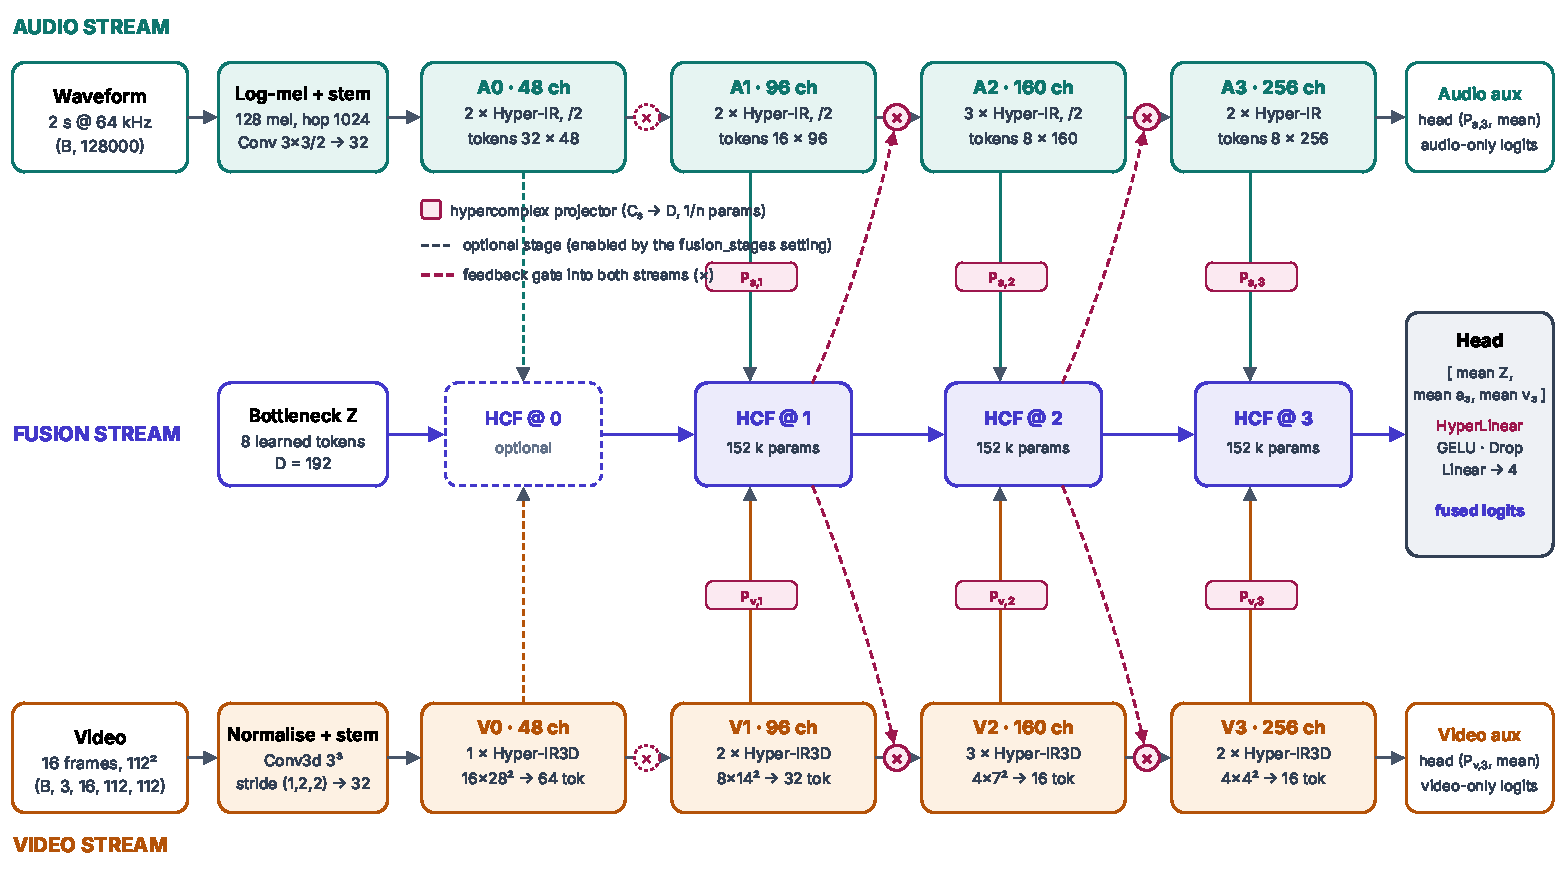
\includegraphics[width=\textwidth]{figures/arch_overview.pdf}
  \caption{HyperAVNet (default configuration: quaternion algebra, fusion stages $\mathcal{S}=\{1,2,3\}$,
  feedback enabled). Stage tokens of the audio and video backbones are projected by hypercomplex
  projectors $P_{a,s}$ and $P_{v,s}$ into a $D$-dimensional fusion space, where HCF blocks update the
  bottleneck tokens $\mathbf{Z}$. After each fused stage $s<S-1$, a zero-initialised gate ($\times$)
  modulates both streams. The classifier reads the pooled bottleneck and the pooled last-stage
  tokens; auxiliary heads supervise each modality on its own. Token shapes are for one 2\,s clip and
  $16\times112^{2}$ frames.}
  \label{fig:overview}
\end{figure*}

\subsection{Hypercomplex layers}
\label{sec:hyper}
Let $\mathbb{A}_n$ be a hypercomplex algebra of dimension $n\in\{2,4,8,16\}$ (complex numbers,
quaternions, octonions, sedenions, obtained by the Cayley--Dickson construction), with basis
$\{e_0,\dots,e_{n-1}\}$ and multiplication table
\begin{equation}
  e_i\,e_j = \sigma_{ij}\, e_{\pi(i,j)},
  \label{eq:table}
\end{equation}
with signs $\sigma_{ij}\in\{-1,+1\}$ and indices $\pi(i,j)\in\{0,\dots,n-1\}$.
A feature vector $\mathbf{x}\in\mathbb{R}^{d_{\mathrm{in}}}$ is split into $n$ components,
$\mathbf{x}=[\mathbf{x}_0;\dots;\mathbf{x}_{n-1}]$ with $\mathbf{x}_j\in\mathbb{R}^{d_{\mathrm{in}}/n}$,
i.e.\ it is read as $\sum_j \mathbf{x}_j e_j$. A hypercomplex weight
$\mathbf{W}=\sum_{k}\mathbf{W}_k e_k$ with real blocks $\mathbf{W}_k\in\mathbb{R}^{(d_{\mathrm{out}}/n)\times(d_{\mathrm{in}}/n)}$
acts on it by the algebra product, which in matrix form is
\begin{equation}
\begin{gathered}
  \mathbf{y}_i = \sum_{j=0}^{n-1} s_{ij}\,\mathbf{W}_{c(i,j)}\,\mathbf{x}_j + \mathbf{b}_i,\\
  \mathbf{K}(\mathbf{W}) = \big[\, s_{ij}\,\mathbf{W}_{c(i,j)} \,\big]_{i,j=0}^{n-1}\in\mathbb{R}^{d_{\mathrm{out}}\times d_{\mathrm{in}}},
\end{gathered}
  \label{eq:hlinear}
\end{equation}
where the block index $c(i,j)$ and sign $s_{ij}$ follow from Eq.~\eqref{eq:table}. For quaternions the
kernel takes the familiar Hamilton form (Fig.~\ref{fig:hamilton}),
\begin{equation}
  \mathbf{K} = \begin{bmatrix}
   \mathbf{W}_0 & \mathbf{W}_1 & \mathbf{W}_2 & \mathbf{W}_3\\
  -\mathbf{W}_1 & \mathbf{W}_0 & \mathbf{W}_3 & -\mathbf{W}_2\\
  -\mathbf{W}_2 & -\mathbf{W}_3 & \mathbf{W}_0 & \mathbf{W}_1\\
  -\mathbf{W}_3 & \mathbf{W}_2 & -\mathbf{W}_1 & \mathbf{W}_0
  \end{bmatrix}.
  \label{eq:hamilton}
\end{equation}
Every output component is thus a signed combination of \emph{every} input component through one
shared set of $n$ blocks, so the layer has
\begin{equation}
  |\theta_{\mathrm{hyper}}| = \tfrac{1}{n}\,d_{\mathrm{in}}d_{\mathrm{out}} + d_{\mathrm{out}}
  \;\;\text{vs.}\;\;
  |\theta_{\mathrm{real}}| = d_{\mathrm{in}}d_{\mathrm{out}} + d_{\mathrm{out}}
  \label{eq:params}
\end{equation}
parameters. A hypercomplex convolution applies the same block structure to the kernel tensor, with
$\mathbf{W}_k\in\mathbb{R}^{(C_{\mathrm{out}}/n)\times(C_{\mathrm{in}}/n)\times k_1\times\dots}$.
Weights are initialised in polar form: a modulus drawn from a $\chi$ distribution with $n$ degrees of
freedom (scaled by the Glorot variance), a uniform phase, and a unit-norm imaginary direction
\cite{bojesomo2024hypercomplex}. We write $\mathcal{H}_n(\cdot)$ for a hypercomplex linear or
convolutional layer. With $n=1$ it reduces to the real layer, which gives a matched real-valued
ablation with an identical code path.

\paragraph{Deployment.} Building $\mathbf{K}$ in Eq.~\eqref{eq:hlinear} at every forward pass
is only needed while training. After training, every $\mathcal{H}_n$ is \emph{reparameterised} into a
dense layer with weight $\mathbf{K}(\mathbf{W})$. The outputs are identical, and the run-time
overhead of kernel assembly disappears. The hypercomplex structure therefore reduces the number of
stored and optimised parameters (and the model's memory and transmission size) by up to $n\times$,
but \emph{not} the multiply--accumulate count, because $\mathbf{K}$ is dense.

\begin{figure}[t]
  \centering
  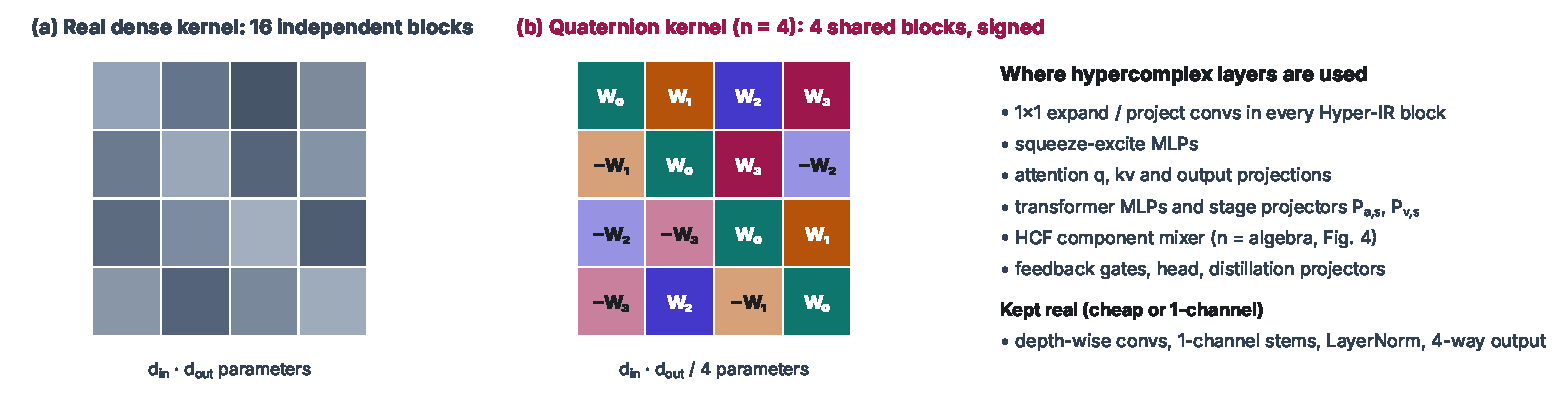
\includegraphics[width=\columnwidth]{figures/hamilton.pdf}
  \caption{Hamilton-product weight sharing. (a) A real kernel has $n^{2}$ independent blocks.
  (b) A quaternion kernel ($n=4$) re-uses four blocks with fixed signs (Eq.~\eqref{eq:hamilton}),
  which cuts the parameter count by $4\times$.}
  \label{fig:hamilton}
\end{figure}

\subsection{Hypercomplex backbones and stage tokens}
\label{sec:backbones}
\paragraph{Hyper-IR block.} Both backbones stack hypercomplex inverted-residual blocks
(Fig.~\ref{fig:hyperir}). For an input $\mathbf{h}\in\mathbb{R}^{C\times\Omega}$ ($\Omega$ is the 2-D
time--frequency grid for audio and the 3-D space--time grid for video) and expansion ratio $r=4$:
\begin{equation}
\begin{aligned}
  \mathbf{u} &= \operatorname{SiLU}\big(\operatorname{BN}(\mathcal{H}_n^{1\times1}(\mathbf{h}))\big)\in\mathbb{R}^{rC\times\Omega},\\
  \mathbf{v} &= \operatorname{SiLU}\big(\operatorname{BN}(\operatorname{DWConv}_{3}(\mathbf{u}))\big),\\
  \mathbf{w} &= \mathbf{v}\odot\sigma\big(\mathcal{H}_n(\operatorname{SiLU}(\mathcal{H}_n(\operatorname{GAP}(\mathbf{v}))))\big),\\
  \mathbf{h}' &= \mathbf{h} + \operatorname{DropPath}\big(\operatorname{BN}(\mathcal{H}_n^{1\times1}(\mathbf{w}))\big).
\end{aligned}
  \label{eq:hyperir}
\end{equation}
The two point-wise convolutions hold almost all of a block's parameters, so they are hypercomplex. The
depth-wise convolution stays real; it accounts for about 1\% of the parameters. The residual is used
when the shape is preserved.

\paragraph{Audio stream.} The waveform is converted to a log-mel spectrogram with the U-FFIA settings
(Hann window 2048, hop 1024, 128 mel bins at 64\,kHz, so a 2\,s clip gives $128\times126$),
normalised per mel bin by batch normalisation and augmented with SpecAugment during training. A
$3{\times}3$ stride-2 stem is followed by four Hyper-IR stages $s=0,\dots,3$ with widths
$(48,96,160,256)$ and depths $(2,2,3,2)$. A stage map $\mathbf{h}^{a}_{s}\in\mathbb{R}^{C_s\times T_s\times F_s}$
becomes time tokens by pooling over frequency:
\begin{equation}
  \mathbf{a}_s = \big[\operatorname{mean}_{F}(\mathbf{h}^{a}_s) + \operatorname{max}_{F}(\mathbf{h}^{a}_s)\big]^{\top}\in\mathbb{R}^{T_s\times C_s}.
  \label{eq:audiotokens}
\end{equation}
The max term keeps the short impulsive transients of feeding (chewing, tail slaps).

\paragraph{Video stream.} The frames are normalised and passed through a $3{\times}3{\times}3$ stem
(spatial stride 2) and four 3-D Hyper-IR stages of the same widths, with depths $(1,2,3,2)$ and
strides $(1,2,2)$, $(2,2,2)$, $(2,2,2)$, $(1,2,2)$. A stage map
$\mathbf{h}^{v}_{s}\in\mathbb{R}^{C_s\times T_s\times H_s\times W_s}$ is pooled to a $2\times2$ spatial grid
per time step, $\mathbf{v}_s\in\mathbb{R}^{4T_s\times C_s}$. This keeps coarse location (where the fish
aggregate) at a small token count.

\begin{figure}[t]
  \centering
  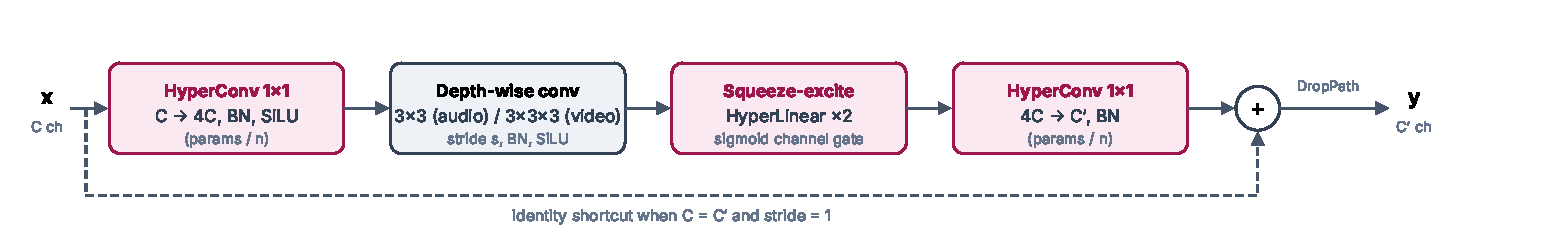
\includegraphics[width=\columnwidth]{figures/hyper_ir.pdf}
  \caption{Hypercomplex inverted-residual (Hyper-IR) block, Eq.~\eqref{eq:hyperir}. Hypercomplex
  layers are shaded; the depth-wise convolution is real.}
  \label{fig:hyperir}
\end{figure}

\paragraph{Pretrained backbones.} Any pretrained network can replace a student backbone if it exposes
four stages in the same token format. We use this for the teachers and for the teacher ablation
(Sec.~\ref{sec:setup}): PANNs CNN10/CNN14~\cite{kong2020panns}, EfficientAT~\cite{schmid2023efficientat},
AST~\cite{gong2021ast}, S3D~\cite{xie2018s3d}, X3D~\cite{feichtenhofer2020x3d},
MoViNet~\cite{kondratyuk2021movinets} and VideoMAE~\cite{tong2022videomae}. Their intermediate layers
supply the stage tokens.

\subsection{Hypercomplex component fusion}
\label{sec:hcf}
\paragraph{Projection.} Stage tokens are mapped into a shared $D$-dimensional space by hypercomplex
projectors with a learned modality embedding:
\begin{equation}
  \mathbf{A}_s = \operatorname{LN}\!\big(\mathcal{H}_n(\mathbf{a}_s)\big) + \mathbf{m}^{a},\qquad
  \mathbf{V}_s = \operatorname{LN}\!\big(\mathcal{H}_n(\mathbf{v}_s)\big) + \mathbf{m}^{v}.
  \label{eq:proj}
\end{equation}

\paragraph{Bottleneck state.} The fused representation lives in $N_b$ learned bottleneck tokens
$\mathbf{Z}\in\mathbb{R}^{N_b\times D}$ (we use $N_b=8$, $D=192$), shared across stages.

\paragraph{HCF block.} At a fusion stage $s$, the bottleneck first reads each modality with its own
hypercomplex cross-attention:
\begin{equation}
\begin{aligned}
  \mathbf{Z}^{a} &= \mathbf{Z} + \operatorname{XAttn}_{n}\big(\operatorname{LN}\mathbf{Z},\,\operatorname{LN}\mathbf{A}_s\big),\\
  \mathbf{Z}^{v} &= \mathbf{Z} + \operatorname{XAttn}_{n}\big(\operatorname{LN}\mathbf{Z},\,\operatorname{LN}\mathbf{V}_s\big),
\end{aligned}
  \label{eq:xattn}
\end{equation}
where $\operatorname{XAttn}_n$ is multi-head attention whose query, key, value and output projections
are hypercomplex (shown for one head of width $d_h$):
\begin{equation*}
  \operatorname{XAttn}_n(\mathbf{Q},\mathbf{C})=\mathcal{H}_n\Big(\operatorname{softmax}\Big(\tfrac{\mathcal{H}_n(\mathbf{Q})\,\mathcal{H}_n(\mathbf{C})^{\top}}{\sqrt{d_h}}\Big)\mathcal{H}_n(\mathbf{C})\Big).
\end{equation*} The shared
state, the two modality views and their interaction then form the components of one element of
$\mathbb{A}_m$:
\begin{equation}
  \mathbf{q} = \mathbf{Z}\,e_0 + \mathbf{Z}^{a}\,e_1 + \mathbf{Z}^{v}\,e_2 + \big(\hat{\mathbf{Z}}^{a}\odot\hat{\mathbf{Z}}^{v}\big)\,e_3,
  \label{eq:components}
\end{equation}
for $m=4$,
with $\hat{\cdot}=\operatorname{LN}(\cdot)$. The octonion variant ($m=8$) appends
$(\mathbf{Z}^{a}-\mathbf{Z}^{v})e_4$, $(\hat{\mathbf{Z}}\odot\hat{\mathbf{Z}}^{a})e_5$,
$(\hat{\mathbf{Z}}\odot\hat{\mathbf{Z}}^{v})e_6$ and
$(\hat{\mathbf{Z}}\odot\hat{\mathbf{Z}}^{a}\odot\hat{\mathbf{Z}}^{v})e_7$; the complex variant ($m=2$) uses
$(\mathbf{Z}^{a},\mathbf{Z}^{v})$. The components are mixed by a single Hamilton product, followed by a
hypercomplex MLP:
\begin{equation}
\begin{aligned}
  \mathbf{Z} &\leftarrow \mathbf{Z} + \boldsymbol{\gamma}_1\odot \mathcal{H}_m(\mathbf{q}),\\
  \mathbf{Z} &\leftarrow \mathbf{Z} + \boldsymbol{\gamma}_2\odot \operatorname{MLP}_n(\operatorname{LN}\mathbf{Z}),
\end{aligned}
  \label{eq:mix}
\end{equation}
where $\mathcal{H}_m:\mathbb{R}^{mD}\to\mathbb{R}^{D}$ is a hypercomplex linear layer of algebra
$\mathbb{A}_m$ and $\boldsymbol{\gamma}_{1,2}$ are LayerScale vectors~\cite{touvron2021cait}, initialised to
$10^{-2}$. By Eq.~\eqref{eq:hlinear}, each output component of $\mathcal{H}_m$ is a signed mixture of
the shared state, both modality views and their multiplicative agreement, all through one set of
$m$ blocks. The mixer has $D^{2}$ parameters \emph{for every} $m$, against $mD^{2}$ for a dense mixer, so
the octonion variant adds four interaction terms at no parameter cost. Unlike attention bottlenecks
that attend to the modalities one after the other~\cite{nagrani2021mbt}, HCF reads both modalities
in parallel and combines them in one algebraic product (Fig.~\ref{fig:hcf}).

\begin{figure*}[t]
  \centering
  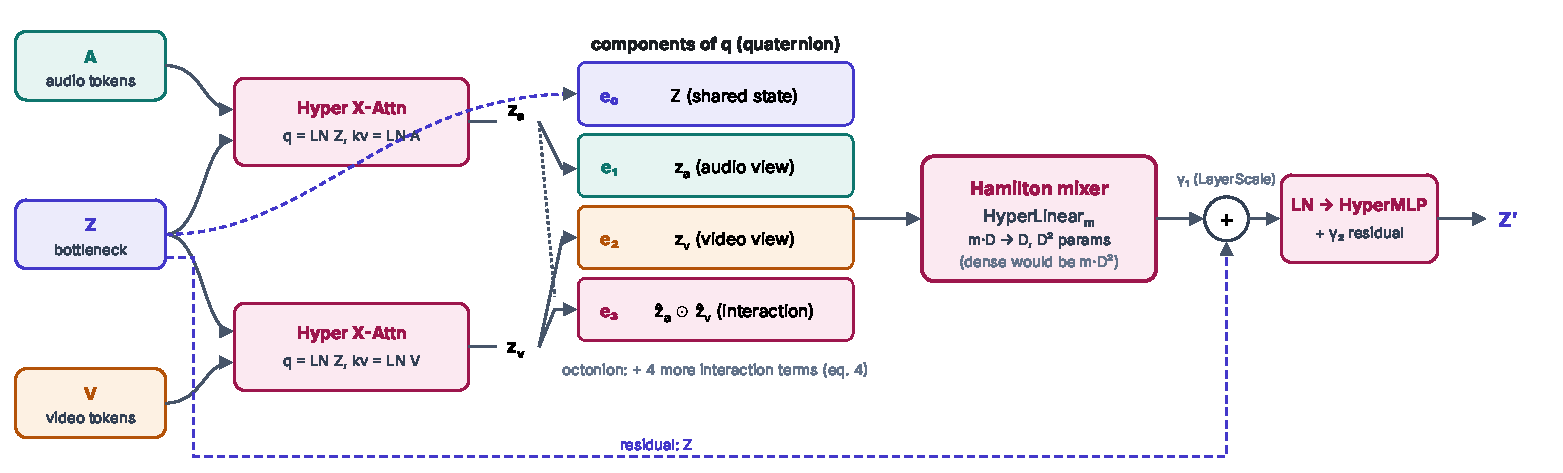
\includegraphics[width=0.9\textwidth]{figures/hcf_block.pdf}
  \caption{Hypercomplex component fusion (HCF), Eqs.~\eqref{eq:xattn}--\eqref{eq:mix}. The modality
  views and their interaction are the components of one quaternion and are mixed by a single
  Hamilton product.}
  \label{fig:hcf}
\end{figure*}

\subsection{Deep-to-early fusion schedule with cross-modal feedback}
\label{sec:schedule}
The set $\mathcal{S}\subseteq\{0,\dots,S-1\}$ selects the stages at which an HCF block is attached:
\begin{equation}
  \mathbf{Z}^{(s+1)} = \begin{cases}\operatorname{HCF}_s\big(\mathbf{Z}^{(s)},\mathbf{A}_s,\mathbf{V}_s\big), & s\in\mathcal{S},\\ \mathbf{Z}^{(s)}, & \text{otherwise,}\end{cases}
  \label{eq:schedule}
\end{equation}
with $\mathbf{Z}^{(0)}=\mathbf{Z}_{\mathrm{init}}$ the learned bottleneck tokens.
Varying $\mathcal{S}$ from $\{S-1\}$ (late fusion) through $\{S-2,S-1\}$ and so on to $\{0,\dots,S-1\}$
gives a controlled \emph{deep-to-early} study of where audio--visual fusion helps. Because the student
backbones are executed stage by stage, the fused state is also fed back into both streams after each
fused stage $s<S-1$:
\begin{equation}
  \mathbf{h}^{m}_s \leftarrow \mathbf{h}^{m}_s\odot\big(1+\tanh(\mathcal{G}^{m}_s\,\bar{\mathbf{z}}^{(s+1)})\big),\quad m\in\{a,v\},
  \label{eq:feedback}
\end{equation}
where $\bar{\mathbf{z}}=\operatorname{mean}_{N_b}(\mathbf{Z})$, the gates
$\mathcal{G}^{m}_s$ are hypercomplex linear maps $\mathbb{R}^{D}\to\mathbb{R}^{C_s}$, and the
product broadcasts over $\Omega$. The gates are \emph{initialised to zero}, so training starts exactly
at the feedback-free model. The network then learns how strongly each modality should condition the
other's later features. This is genuine early fusion, as opposed to fusing independently computed
features.

\subsection{Prediction heads and modality dropout}
\label{sec:heads}
With $\bar{\mathbf{z}}=\operatorname{mean}(\operatorname{LN}\mathbf{Z}^{(S)})$,
$\bar{\mathbf{a}}=\operatorname{mean}(\operatorname{LN}\mathbf{A}_{S-1})$ and
$\bar{\mathbf{v}}=\operatorname{mean}(\operatorname{LN}\mathbf{V}_{S-1})$, the fused and auxiliary logits are
\begin{equation}
\begin{gathered}
  \boldsymbol{\ell} = \mathbf{W}_o\,\operatorname{GELU}\big(\mathcal{H}_n[\bar{\mathbf{z}};\,\mu_a\bar{\mathbf{a}};\,\mu_v\bar{\mathbf{v}}]\big),\\
  \boldsymbol{\ell}^{a} = \mathbf{W}_a\bar{\mathbf{a}},\qquad \boldsymbol{\ell}^{v} = \mathbf{W}_v\bar{\mathbf{v}}.
\end{gathered}
  \label{eq:heads}
\end{equation}
Here $\mu_a,\mu_v\in\{0,1\}$ are per-sample modality masks. During training,
$(\mu_a,\mu_v)=(0,1)$ with probability $p$, $(1,0)$ with probability $p$, and $(1,1)$ otherwise. In the
notation of~\cite{cui2024uffia}, $p_{av}=1-2p$ and $p_a=p_v=p$. The same mask multiplies every fusion
input $\mathbf{A}_s,\mathbf{V}_s$, so a dropped modality is absent everywhere. The auxiliary heads always see
their own modality, which keeps both branches trained regardless of $p$. At test time, forcing
$\mu_a=0$ or $\mu_v=0$ evaluates the model with a missing modality.

\subsection{Training objective and multi-level distillation}
\label{sec:objective}
The supervised loss combines label-smoothed cross-entropy on the fused logits with the two
auxiliary terms:
\begin{equation}
  \mathcal{L}_{\mathrm{sup}} = \operatorname{CE}_{\epsilon}(\boldsymbol{\ell},y)
   + \tfrac{\lambda_{\mathrm{aux}}}{2}\!\!\sum_{m\in\{a,v\}}\!\!\operatorname{CE}_{\epsilon}(\boldsymbol{\ell}^{m},y).
  \label{eq:sup}
\end{equation}
A frozen teacher $g$ with the same output structure (pretrained backbones and HCF fusion) provides
three further signals. At the \emph{logit level}, with temperature $\tau$:
\begin{equation}
  \mathcal{L}_{\mathrm{KD}} = \tau^{2}\,\mathrm{KL}\big(\boldsymbol{\ell}^{g}\,\|\,\boldsymbol{\ell}\big)_{\tau}
   + \tfrac{\lambda_{u}\tau^{2}}{2}\!\!\sum_{m\in\{a,v\}}\!\!\mathrm{KL}\big(\boldsymbol{\ell}^{g,m}\,\|\,\boldsymbol{\ell}^{m}\big)_{\tau},
  \label{eq:kd}
\end{equation}
with $\mathrm{KL}(\mathbf{u}\,\|\,\mathbf{w})_{\tau}=\mathrm{KL}\big(\operatorname{softmax}(\mathbf{u}/\tau)\,\|\,\operatorname{softmax}(\mathbf{w}/\tau)\big)$,
which distils each unimodal head from its counterpart in the teacher. U-FFIA's variant~\cite{cui2024uffia}
softens only the teacher, $\mathrm{KL}(\operatorname{softmax}(\boldsymbol{\ell}^{g}/\tau)\,\|\,\operatorname{softmax}(\boldsymbol{\ell}))$,
and is evaluated as an ablation. At the \emph{embedding level}, small hypercomplex projectors
$\mathcal{P}_k$ align the student's pooled embeddings with the teacher's:
\begin{equation}
  \mathcal{L}_{\mathrm{feat}} = \tfrac{1}{3}\!\!\sum_{k\in\{\bar{\mathbf{z}},\bar{\mathbf{a}},\bar{\mathbf{v}}\}}\!\!
  \big(1-\cos(\mathcal{P}_k(k),\,k^{g})\big).
  \label{eq:feat}
\end{equation}
At the \emph{relation level}~\cite{park2019rkd}, the within-batch similarity structure of the fused
embeddings is matched:
\begin{equation}
  \mathcal{L}_{\mathrm{rel}} = \operatorname{SmoothL1}\big(\mathbf{R}(\bar{\mathbf{z}}_{1:B}),\,\mathbf{R}(\bar{\mathbf{z}}^{g}_{1:B})\big),
  \label{eq:rel}
\end{equation}
where $\mathbf{R}(\mathbf{U})_{ij}=\mathbf{u}_i^{\top}\mathbf{u}_j/(\|\mathbf{u}_i\|\|\mathbf{u}_j\|)$ is the cosine-similarity matrix of a batch of size $B$.
The full objective is
\begin{equation}
  \mathcal{L} = \mathcal{L}_{\mathrm{sup}} + \alpha\,\mathcal{L}_{\mathrm{KD}} + \beta\,\mathcal{L}_{\mathrm{feat}} + \gamma\,\mathcal{L}_{\mathrm{rel}},
  \label{eq:total}
\end{equation}
with $\epsilon=0.1$, $\lambda_{\mathrm{aux}}=0.3$, $\lambda_u=0.5$, $\tau=2$, $\alpha=0.7$, $\beta=1$ and $\gamma=0.5$.
Training proceeds in two stages: the teacher is trained with $\mathcal{L}_{\mathrm{sup}}$ and frozen, then
the student is trained with Eq.~\eqref{eq:total}.

\begin{figure*}[t]
  \centering
  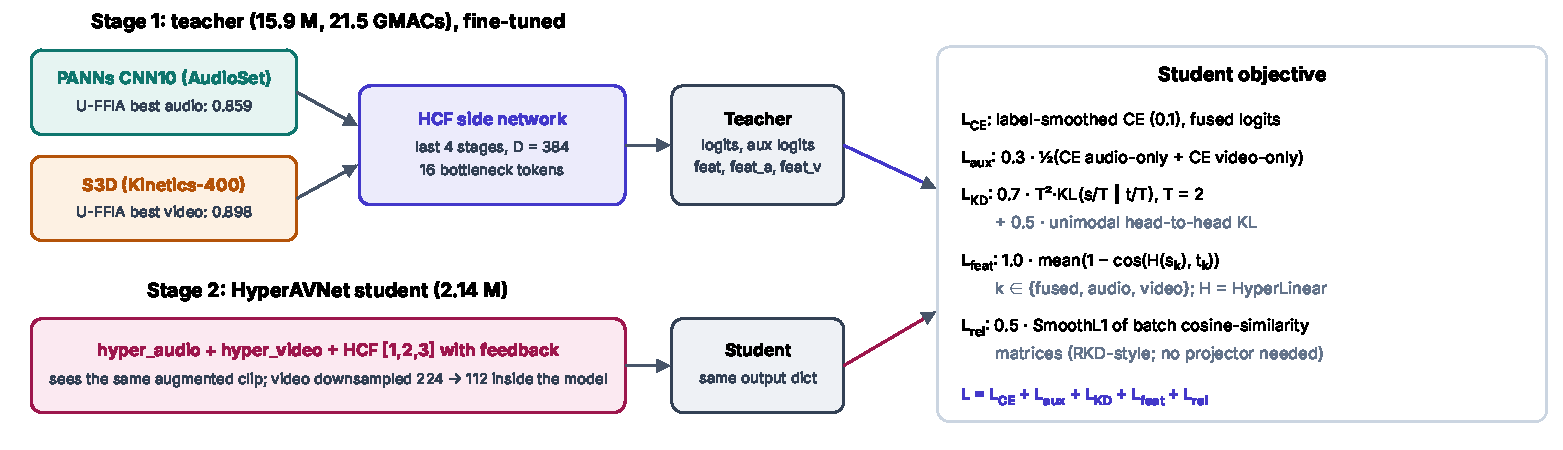
\includegraphics[width=0.92\textwidth]{figures/distillation.pdf}
  \caption{Two-stage training. A teacher built from pretrained audio and video backbones and HCF fusion
  is trained first and frozen. The HyperAVNet student is then trained with the supervised loss plus
  logit-, embedding- and relation-level distillation (Eq.~\eqref{eq:total}).}
  \label{fig:distill}
\end{figure*}

\subsection{Complexity}
\label{sec:complexity}
By Eq.~\eqref{eq:params}, every hypercomplex projection stores $1/n$ of the real parameters. Only the
stems, the depth-wise convolutions, normalisation layers and the final $4$-way classifier stay real.
For the default student ($n=4$), the network has 2.14\,M parameters against 7.88\,M for the identical
real network ($n=1$), and 1.24\,M (octonion) or 0.78\,M (sedenion) for higher algebras. Compute is
1.18\,GMACs per clip for every $n$ (16 frames at $112^{2}$ and 2\,s of audio). The added cost of a
fusion stage is about 0.17\,M parameters and under 0.02\,GMACs.
 % ============================================================================
%  Experimental set-up -- % ============================================================================
%  Experimental set-up -- % ============================================================================
%  Experimental set-up -- \input{sections/experiments}
% ============================================================================
\section{Experimental Set-up}
\label{sec:setup}

\paragraph{Dataset.} AV-FFIA~\cite{cui2024uffia} contains synchronised two-second audio--video clips of
\textit{Oplegnathus punctatus} feeding in a recirculating tank, labelled by a feeding technician into
four intensities. Audio was recorded by a hydrophone at 256\,kHz (used at 64\,kHz), and video by an
overhead camera at 25\,fps. The paper describes 27,000 clips (6,750 per class). The published
splits~\cite{cui2024uffia}, later re-implementations~\cite{dynagate2026,hmmfnet2026} and the public
release disagree on the clip count, so we report the number of clips we used (\todo{N clips}) and
release our split files.

\paragraph{Evaluation protocols.} Published AV-FFIA results use incompatible protocols, so we
evaluate under three and state the protocol with every number.
(i)~\emph{Official split}: the U-FFIA rule (each class shuffled with seed 25; 700 test and 700
validation clips per class; the rest for training), applied to a \emph{sorted} file list so that the
split is deterministic. We publish its hash. This is the protocol of~\cite{cui2024uffia,dynagate2026}.
(ii)~\emph{5-fold stratified cross-validation}, as in~\cite{hmmfnet2026}; one fold is the test set, and
one-eighth of the remaining clips is held out for model selection.
(iii)~\emph{Session-disjoint split}: whole recording sessions (dates) are assigned to the train,
validation or test set. The clips are two-second segments of one-minute recordings, so every
clip-level random split, including (i) and (ii), places near-duplicate neighbours in both train and
test. Protocol (iii) measures generalisation to unseen sessions; to our knowledge it is the first
leakage-free result on AV-FFIA.

\paragraph{Pre-processing and augmentation.} Audio is resampled to 64\,kHz and cropped or padded to 2\,s.
Log-mel spectrograms follow U-FFIA (window 2048, hop 1024, 128 bins). Training uses SpecAugment
(two frequency masks of width $\le8$ and two time masks of width $\le16$), random gain
($\pm6$\,dB) and circular time shift. Sixteen frames are sampled uniformly per clip and resized to a
short side of 128 (student) or 256 (teacher), then randomly cropped to $112^{2}$ (student) or $224^{2}$
(teacher), with horizontal flips and brightness/contrast jitter. Evaluation uses a centre crop and no
augmentation. Under distillation the student receives the teacher's $224^{2}$ input and resizes it to
$112^{2}$ internally, so both models see exactly the same augmented clip.

\paragraph{Teachers.} The default teacher pairs the strongest pretrained single-modality models on
AV-FFIA~\cite{cui2024uffia}: AudioSet PANNs CNN10~\cite{kong2020panns} and Kinetics-400
S3D~\cite{xie2018s3d}. Their last four stages are fused by HCF ($\mathcal{S}=\{0,1,2,3\}$, $D=384$,
$N_b=16$), giving 15.9\,M parameters and 21.5\,GMACs. The teacher ablation (Table~\ref{tab:teachers})
varies the backbone pair over ten configurations (T1--T10), changing one modality at a time where
possible:
\begin{itemize}
  \item \emph{audio}: CNN10, CNN14, an ImageNet EfficientNet-B0 on mel spectrograms, AST~\cite{gong2021ast}, and EfficientAT
mn10~\cite{schmid2023efficientat};
  \item \emph{video}: S3D, R(2+1)D-18, a per-frame ConvNeXt-T with a hypercomplex temporal adapter,
X3D-M~\cite{feichtenhofer2020x3d}, VideoMAE-B~\cite{tong2022videomae}, and MoViNet-A0~\cite{kondratyuk2021movinets}.
\end{itemize}
T10 reproduces the EfficientAT + MoViNet-A0 teacher pair of~\cite{hmkd2026}. Each teacher is trained with
the same recipe, and a student is distilled from each.

\paragraph{Student variants.} HyperAVNet-Q is the fully hypercomplex student of Sec.~\ref{sec:method},
trained from scratch. HyperAVNet-P keeps the hypercomplex projectors, HCF fusion and heads, but replaces
the student backbones with compact pretrained networks: EfficientAT mn04~\cite{schmid2023efficientat} for
audio and MoViNet-A0~\cite{kondratyuk2021movinets} for video at $172^{2}$. This gives 1.89\,M parameters
and 0.88\,GMACs, and tests how much of the gap to the teacher is due to pretraining rather than
architecture.

\paragraph{Baselines.} We compare against the results published by
\cite{cui2024uffia,acafnet2025,dynagate2026,hmmfnet2026,hmkd2026,ldmf2026}, each with its stated protocol,
and against models we re-train under our protocol: a real-valued late-concatenation model with the
teacher's backbones, the teachers, and HyperAVNet without distillation. Re-runs of the same
cross-attention baseline in different works vary by about 1.5 percentage points (91.7\%~\cite{cui2024uffia},
92.4\%~\cite{dynagate2026}, 93.4\%~\cite{acafnet2025}). We therefore regard differences of that size
across papers as inconclusive, and draw conclusions only from comparisons within our own pipeline.

\paragraph{Implementation details.} Models are trained with AdamW ($\beta=(0.9,0.999)$, weight decay
0.05, none on normalisation, bias and token parameters), batch size 32 (student) or 16 (teacher), and a
peak learning rate of $10^{-3}$ (student) or $3\times10^{-4}$ (teacher; pretrained weights at
$0.3\times$). The schedule is a cosine decay with a two-epoch warm-up over 40 (student) or 30
(teacher) epochs. We use bf16 mixed precision, gradient clipping at 5, stochastic depth 0.1 and modality
dropout $p=0.1$. Model selection uses validation accuracy of an exponential moving average of the
weights (decay 0.999), and the test set is evaluated once. Every configuration is run with three
seeds (the split is fixed), and we report mean $\pm$ standard deviation. Parameters are counted from
the trained model. Compute is counted with PyTorch's \texttt{FlopCounterMode} and reported in MACs
(1\,MAC $=$ 2\,FLOPs), which is the unit U-FFIA calls ``FLOPs''. We confirmed this by measuring
torchvision S3D at $20\times224^{2}$ as 22.4\,GMACs, against 22.8 reported in~\cite{cui2024uffia}.

\paragraph{Metrics and robustness protocol.} We report accuracy (the standard metric in FFIA) and
macro-F1, plus audio-only and video-only accuracy from the auxiliary heads. Robustness follows
\cite{cui2024uffia}: noise is added to the whole audio clip at an SNR of $-10$, $-5$, $0$, $10$ or 20\,dB,
using bubble and pump recordings (\todo{or white noise if the recordings are unavailable; state
which}). Video is corrupted by darkness (intensities $\times0.25$) and additive Gaussian noise
($\sigma^{2}=0.2$). We also evaluate with the audio or the video absent ($\mu_a=0$ or $\mu_v=0$ in
Eq.~\eqref{eq:heads}). All corruptions are seeded, so every model sees identical corrupted inputs.

% ============================================================================
\section{Experimental Set-up}
\label{sec:setup}

\paragraph{Dataset.} AV-FFIA~\cite{cui2024uffia} contains synchronised two-second audio--video clips of
\textit{Oplegnathus punctatus} feeding in a recirculating tank, labelled by a feeding technician into
four intensities. Audio was recorded by a hydrophone at 256\,kHz (used at 64\,kHz), and video by an
overhead camera at 25\,fps. The paper describes 27,000 clips (6,750 per class). The published
splits~\cite{cui2024uffia}, later re-implementations~\cite{dynagate2026,hmmfnet2026} and the public
release disagree on the clip count, so we report the number of clips we used (\todo{N clips}) and
release our split files.

\paragraph{Evaluation protocols.} Published AV-FFIA results use incompatible protocols, so we
evaluate under three and state the protocol with every number.
(i)~\emph{Official split}: the U-FFIA rule (each class shuffled with seed 25; 700 test and 700
validation clips per class; the rest for training), applied to a \emph{sorted} file list so that the
split is deterministic. We publish its hash. This is the protocol of~\cite{cui2024uffia,dynagate2026}.
(ii)~\emph{5-fold stratified cross-validation}, as in~\cite{hmmfnet2026}; one fold is the test set, and
one-eighth of the remaining clips is held out for model selection.
(iii)~\emph{Session-disjoint split}: whole recording sessions (dates) are assigned to the train,
validation or test set. The clips are two-second segments of one-minute recordings, so every
clip-level random split, including (i) and (ii), places near-duplicate neighbours in both train and
test. Protocol (iii) measures generalisation to unseen sessions; to our knowledge it is the first
leakage-free result on AV-FFIA.

\paragraph{Pre-processing and augmentation.} Audio is resampled to 64\,kHz and cropped or padded to 2\,s.
Log-mel spectrograms follow U-FFIA (window 2048, hop 1024, 128 bins). Training uses SpecAugment
(two frequency masks of width $\le8$ and two time masks of width $\le16$), random gain
($\pm6$\,dB) and circular time shift. Sixteen frames are sampled uniformly per clip and resized to a
short side of 128 (student) or 256 (teacher), then randomly cropped to $112^{2}$ (student) or $224^{2}$
(teacher), with horizontal flips and brightness/contrast jitter. Evaluation uses a centre crop and no
augmentation. Under distillation the student receives the teacher's $224^{2}$ input and resizes it to
$112^{2}$ internally, so both models see exactly the same augmented clip.

\paragraph{Teachers.} The default teacher pairs the strongest pretrained single-modality models on
AV-FFIA~\cite{cui2024uffia}: AudioSet PANNs CNN10~\cite{kong2020panns} and Kinetics-400
S3D~\cite{xie2018s3d}. Their last four stages are fused by HCF ($\mathcal{S}=\{0,1,2,3\}$, $D=384$,
$N_b=16$), giving 15.9\,M parameters and 21.5\,GMACs. The teacher ablation (Table~\ref{tab:teachers})
varies the backbone pair over ten configurations (T1--T10), changing one modality at a time where
possible:
\begin{itemize}
  \item \emph{audio}: CNN10, CNN14, an ImageNet EfficientNet-B0 on mel spectrograms, AST~\cite{gong2021ast}, and EfficientAT
mn10~\cite{schmid2023efficientat};
  \item \emph{video}: S3D, R(2+1)D-18, a per-frame ConvNeXt-T with a hypercomplex temporal adapter,
X3D-M~\cite{feichtenhofer2020x3d}, VideoMAE-B~\cite{tong2022videomae}, and MoViNet-A0~\cite{kondratyuk2021movinets}.
\end{itemize}
T10 reproduces the EfficientAT + MoViNet-A0 teacher pair of~\cite{hmkd2026}. Each teacher is trained with
the same recipe, and a student is distilled from each.

\paragraph{Student variants.} HyperAVNet-Q is the fully hypercomplex student of Sec.~\ref{sec:method},
trained from scratch. HyperAVNet-P keeps the hypercomplex projectors, HCF fusion and heads, but replaces
the student backbones with compact pretrained networks: EfficientAT mn04~\cite{schmid2023efficientat} for
audio and MoViNet-A0~\cite{kondratyuk2021movinets} for video at $172^{2}$. This gives 1.89\,M parameters
and 0.88\,GMACs, and tests how much of the gap to the teacher is due to pretraining rather than
architecture.

\paragraph{Baselines.} We compare against the results published by
\cite{cui2024uffia,acafnet2025,dynagate2026,hmmfnet2026,hmkd2026,ldmf2026}, each with its stated protocol,
and against models we re-train under our protocol: a real-valued late-concatenation model with the
teacher's backbones, the teachers, and HyperAVNet without distillation. Re-runs of the same
cross-attention baseline in different works vary by about 1.5 percentage points (91.7\%~\cite{cui2024uffia},
92.4\%~\cite{dynagate2026}, 93.4\%~\cite{acafnet2025}). We therefore regard differences of that size
across papers as inconclusive, and draw conclusions only from comparisons within our own pipeline.

\paragraph{Implementation details.} Models are trained with AdamW ($\beta=(0.9,0.999)$, weight decay
0.05, none on normalisation, bias and token parameters), batch size 32 (student) or 16 (teacher), and a
peak learning rate of $10^{-3}$ (student) or $3\times10^{-4}$ (teacher; pretrained weights at
$0.3\times$). The schedule is a cosine decay with a two-epoch warm-up over 40 (student) or 30
(teacher) epochs. We use bf16 mixed precision, gradient clipping at 5, stochastic depth 0.1 and modality
dropout $p=0.1$. Model selection uses validation accuracy of an exponential moving average of the
weights (decay 0.999), and the test set is evaluated once. Every configuration is run with three
seeds (the split is fixed), and we report mean $\pm$ standard deviation. Parameters are counted from
the trained model. Compute is counted with PyTorch's \texttt{FlopCounterMode} and reported in MACs
(1\,MAC $=$ 2\,FLOPs), which is the unit U-FFIA calls ``FLOPs''. We confirmed this by measuring
torchvision S3D at $20\times224^{2}$ as 22.4\,GMACs, against 22.8 reported in~\cite{cui2024uffia}.

\paragraph{Metrics and robustness protocol.} We report accuracy (the standard metric in FFIA) and
macro-F1, plus audio-only and video-only accuracy from the auxiliary heads. Robustness follows
\cite{cui2024uffia}: noise is added to the whole audio clip at an SNR of $-10$, $-5$, $0$, $10$ or 20\,dB,
using bubble and pump recordings (\todo{or white noise if the recordings are unavailable; state
which}). Video is corrupted by darkness (intensities $\times0.25$) and additive Gaussian noise
($\sigma^{2}=0.2$). We also evaluate with the audio or the video absent ($\mu_a=0$ or $\mu_v=0$ in
Eq.~\eqref{eq:heads}). All corruptions are seeded, so every model sees identical corrupted inputs.

% ============================================================================
\section{Experimental Set-up}
\label{sec:setup}

\paragraph{Dataset.} AV-FFIA~\cite{cui2024uffia} contains synchronised two-second audio--video clips of
\textit{Oplegnathus punctatus} feeding in a recirculating tank, labelled by a feeding technician into
four intensities. Audio was recorded by a hydrophone at 256\,kHz (used at 64\,kHz), and video by an
overhead camera at 25\,fps. The paper describes 27,000 clips (6,750 per class). The published
splits~\cite{cui2024uffia}, later re-implementations~\cite{dynagate2026,hmmfnet2026} and the public
release disagree on the clip count, so we report the number of clips we used (\todo{N clips}) and
release our split files.

\paragraph{Evaluation protocols.} Published AV-FFIA results use incompatible protocols, so we
evaluate under three and state the protocol with every number.
(i)~\emph{Official split}: the U-FFIA rule (each class shuffled with seed 25; 700 test and 700
validation clips per class; the rest for training), applied to a \emph{sorted} file list so that the
split is deterministic. We publish its hash. This is the protocol of~\cite{cui2024uffia,dynagate2026}.
(ii)~\emph{5-fold stratified cross-validation}, as in~\cite{hmmfnet2026}; one fold is the test set, and
one-eighth of the remaining clips is held out for model selection.
(iii)~\emph{Session-disjoint split}: whole recording sessions (dates) are assigned to the train,
validation or test set. The clips are two-second segments of one-minute recordings, so every
clip-level random split, including (i) and (ii), places near-duplicate neighbours in both train and
test. Protocol (iii) measures generalisation to unseen sessions; to our knowledge it is the first
leakage-free result on AV-FFIA.

\paragraph{Pre-processing and augmentation.} Audio is resampled to 64\,kHz and cropped or padded to 2\,s.
Log-mel spectrograms follow U-FFIA (window 2048, hop 1024, 128 bins). Training uses SpecAugment
(two frequency masks of width $\le8$ and two time masks of width $\le16$), random gain
($\pm6$\,dB) and circular time shift. Sixteen frames are sampled uniformly per clip and resized to a
short side of 128 (student) or 256 (teacher), then randomly cropped to $112^{2}$ (student) or $224^{2}$
(teacher), with horizontal flips and brightness/contrast jitter. Evaluation uses a centre crop and no
augmentation. Under distillation the student receives the teacher's $224^{2}$ input and resizes it to
$112^{2}$ internally, so both models see exactly the same augmented clip.

\paragraph{Teachers.} The default teacher pairs the strongest pretrained single-modality models on
AV-FFIA~\cite{cui2024uffia}: AudioSet PANNs CNN10~\cite{kong2020panns} and Kinetics-400
S3D~\cite{xie2018s3d}. Their last four stages are fused by HCF ($\mathcal{S}=\{0,1,2,3\}$, $D=384$,
$N_b=16$), giving 15.9\,M parameters and 21.5\,GMACs. The teacher ablation (Table~\ref{tab:teachers})
varies the backbone pair over ten configurations (T1--T10), changing one modality at a time where
possible:
\begin{itemize}
  \item \emph{audio}: CNN10, CNN14, an ImageNet EfficientNet-B0 on mel spectrograms, AST~\cite{gong2021ast}, and EfficientAT
mn10~\cite{schmid2023efficientat};
  \item \emph{video}: S3D, R(2+1)D-18, a per-frame ConvNeXt-T with a hypercomplex temporal adapter,
X3D-M~\cite{feichtenhofer2020x3d}, VideoMAE-B~\cite{tong2022videomae}, and MoViNet-A0~\cite{kondratyuk2021movinets}.
\end{itemize}
T10 reproduces the EfficientAT + MoViNet-A0 teacher pair of~\cite{hmkd2026}. Each teacher is trained with
the same recipe, and a student is distilled from each.

\paragraph{Student variants.} HyperAVNet-Q is the fully hypercomplex student of Sec.~\ref{sec:method},
trained from scratch. HyperAVNet-P keeps the hypercomplex projectors, HCF fusion and heads, but replaces
the student backbones with compact pretrained networks: EfficientAT mn04~\cite{schmid2023efficientat} for
audio and MoViNet-A0~\cite{kondratyuk2021movinets} for video at $172^{2}$. This gives 1.89\,M parameters
and 0.88\,GMACs, and tests how much of the gap to the teacher is due to pretraining rather than
architecture.

\paragraph{Baselines.} We compare against the results published by
\cite{cui2024uffia,acafnet2025,dynagate2026,hmmfnet2026,hmkd2026,ldmf2026}, each with its stated protocol,
and against models we re-train under our protocol: a real-valued late-concatenation model with the
teacher's backbones, the teachers, and HyperAVNet without distillation. Re-runs of the same
cross-attention baseline in different works vary by about 1.5 percentage points (91.7\%~\cite{cui2024uffia},
92.4\%~\cite{dynagate2026}, 93.4\%~\cite{acafnet2025}). We therefore regard differences of that size
across papers as inconclusive, and draw conclusions only from comparisons within our own pipeline.

\paragraph{Implementation details.} Models are trained with AdamW ($\beta=(0.9,0.999)$, weight decay
0.05, none on normalisation, bias and token parameters), batch size 32 (student) or 16 (teacher), and a
peak learning rate of $10^{-3}$ (student) or $3\times10^{-4}$ (teacher; pretrained weights at
$0.3\times$). The schedule is a cosine decay with a two-epoch warm-up over 40 (student) or 30
(teacher) epochs. We use bf16 mixed precision, gradient clipping at 5, stochastic depth 0.1 and modality
dropout $p=0.1$. Model selection uses validation accuracy of an exponential moving average of the
weights (decay 0.999), and the test set is evaluated once. Every configuration is run with three
seeds (the split is fixed), and we report mean $\pm$ standard deviation. Parameters are counted from
the trained model. Compute is counted with PyTorch's \texttt{FlopCounterMode} and reported in MACs
(1\,MAC $=$ 2\,FLOPs), which is the unit U-FFIA calls ``FLOPs''. We confirmed this by measuring
torchvision S3D at $20\times224^{2}$ as 22.4\,GMACs, against 22.8 reported in~\cite{cui2024uffia}.

\paragraph{Metrics and robustness protocol.} We report accuracy (the standard metric in FFIA) and
macro-F1, plus audio-only and video-only accuracy from the auxiliary heads. Robustness follows
\cite{cui2024uffia}: noise is added to the whole audio clip at an SNR of $-10$, $-5$, $0$, $10$ or 20\,dB,
using bubble and pump recordings (\todo{or white noise if the recordings are unavailable; state
which}). Video is corrupted by darkness (intensities $\times0.25$) and additive Gaussian noise
($\sigma^{2}=0.2$). We also evaluate with the audio or the video absent ($\mu_a=0$ or $\mu_v=0$ in
Eq.~\eqref{eq:heads}). All corruptions are seeded, so every model sees identical corrupted inputs.
 % ============================================================================
%  Results -- % ============================================================================
%  Results -- % ============================================================================
%  Results -- \input{sections/results}
%  Numbers come from tables/*.tex and tables/macros.tex, generated by
%  scripts/make_paper_assets.py from the run folders. Re-run it after new runs.
%  Sentences marked \todo{} state a claim that must be checked against the
%  final numbers (keep, reverse or delete).
% ============================================================================
\section{Results}
\label{sec:results}

\subsection{Comparison with the state of the art}
\label{sec:main}
Table~\ref{tab:main} lists the published results on AV-FFIA with their protocols, followed by our models
under the official split. The distilled quaternion model, HyperAVNet-Q (KD), reaches
\resOurAcc\,\% accuracy (macro-F1 \resOurFone\,\%) with \resOurParams\,M parameters and
\resOurGMACs\,GMACs per clip. That is 10.1$\times$ fewer parameters and 13.1$\times$ fewer MACs than
U-FFIA~\cite{cui2024uffia}, and 16.4$\times$ / 51.6$\times$ fewer than the cross-attention model.
\todo{Position against the strongest comparable result: DynaGate-AV reports 96.4--96.5\% on the same
official split rule, and HMMF-Net 96.77\% under 5-fold CV (Table~\ref{tab:protocols}). State whether
HyperAVNet exceeds, matches or trails them; LDMF and HMKD use filtered subsets and are not comparable.}
Fig.~\ref{fig:acc_compute} places all models on an accuracy--compute plane.
Its single-modality heads reach \resOurAccA\,\% (audio) and \resOurAccV\,\% (video), against the
best published single-modality models, Pre-CNN10 (85.9\%) and Pretrained-S3D (89.8\%)~\cite{cui2024uffia}.

\begin{table*}[t]
  \centering
  \caption{Comparison on AV-FFIA. Compute is in GMACs per 2\,s clip; U-FFIA's ``FLOPs'' are MACs.
  Published numbers are quoted with their own protocol and are not directly comparable across
  protocols. $^\dagger$Not verified against the full paper (taken from secondary sources). Our
  rows: official split, mean $\pm$ std over three seeds.}
  \label{tab:main}
  \small
  \resizebox{\textwidth}{!}{\input{tables/main.tex}}
\end{table*}

\begin{figure}[t]
  \centering
  \IfFileExists{figures/acc_vs_compute.pdf}{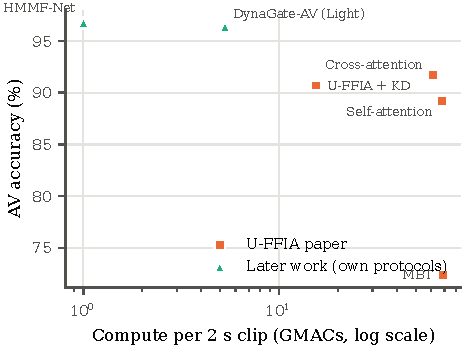
\includegraphics[width=\columnwidth]{figures/acc_vs_compute.pdf}}{\fbox{\parbox{0.9\columnwidth}{\centering run \texttt{scripts/make\_paper\_assets.py}}}}
  \caption{Accuracy versus compute (log scale) on AV-FFIA. Published models are plotted at their
  reported values and protocols; HyperAVNet uses the official split.}
  \label{fig:acc_compute}
\end{figure}

\subsection{Where to fuse: the deep-to-early study}
\label{sec:depth}
Table~\ref{tab:depth} and Fig.~\ref{fig:depth} vary the fusion set $\mathcal{S}$. Late fusion
($\mathcal{S}=\{3\}$) gives \resLateAcc\,\%; progressive fusion from stage~1 gives \resProgAcc\,\%;
the best setting is $\mathcal{S}=\resBestDepth$. Fusion is nearly free in compute: each additional HCF
stage costs about 0.17\,M parameters and under 0.02\,GMACs. Disabling the cross-modal feedback of
Eq.~\eqref{eq:feedback} at $\mathcal{S}=\{1,2,3\}$ gives \resNoFeedbackAcc\,\%.
\todo{Interpret: does accuracy grow as fusion moves earlier, saturate, or peak at mid-level stages
(an inverted U)? Does feedback help, and does the gain concentrate on Weak and Medium? Use the
single-stage rows to locate the most useful depth.}

\begin{table}[t]
  \centering
  \caption{Fusion depth (deep to early) and cross-modal feedback. Mean $\pm$ std, official split.}
  \label{tab:depth}
  \footnotesize
  \setlength{\tabcolsep}{3pt}
  \resizebox{\columnwidth}{!}{\input{tables/ablation_depth.tex}}
\end{table}

\begin{figure}[t]
  \centering
  \IfFileExists{figures/fusion_depth.pdf}{\includegraphics[width=\columnwidth]{figures/fusion_depth.pdf}}{\fbox{\parbox{0.9\columnwidth}{\centering pending runs \texttt{A\_fs*}}}}
  \caption{Accuracy as fusion moves from the last stage to all stages, with and without feedback.}
  \label{fig:depth}
\end{figure}

\subsection{Effect of the hypercomplex algebra}
\label{sec:algebra}
Table~\ref{tab:algebra} and Fig.~\ref{fig:algebra} replace every hypercomplex layer of the network with
algebra $\mathbb{A}_n$. All variants share the architecture and compute and differ only in weight
sharing. The real network ($n=1$, 7.88\,M parameters) reaches \resRealAcc\,\%, the quaternion network
(2.14\,M) \resQuatAcc\,\% and the octonion network (1.24\,M) \resOctAcc\,\%.
\todo{Interpret: if accuracy is maintained or improved down to $n=4$ or $n=8$, the Hamilton
weight sharing acts as a useful structural prior on a dataset of this size; report where accuracy
starts to drop.}

\begin{table}[t]
  \centering
  \caption{Algebra of the whole network. Compute is identical for all $n$.}
  \label{tab:algebra}
  \footnotesize
  \resizebox{\columnwidth}{!}{\input{tables/ablation_algebra.tex}}
\end{table}

\begin{figure}[t]
  \centering
  \IfFileExists{figures/algebra.pdf}{\includegraphics[width=\columnwidth]{figures/algebra.pdf}}{\fbox{\parbox{0.9\columnwidth}{\centering pending runs \texttt{B\_n*}}}}
  \caption{Accuracy against parameter count for real, complex, quaternion, octonion and sedenion networks.}
  \label{fig:algebra}
\end{figure}

\subsection{Fusion operator, regularisers and front-end}
\label{sec:operators}
Table~\ref{tab:ops} compares HCF with a hypercomplex attention bottleneck (MBT) at equal parameters,
and with gated concatenation. HCF with quaternion components gives \resHCFAcc\,\% and MBT
\resMBTAcc\,\%. In~\cite{cui2024uffia}, MBT also trailed cross-attention by a wide margin
(72.4\% vs.\ 91.7\%), which the authors attributed to attending to the modalities one after the other.
\todo{State whether parallel reading plus Hamilton mixing closes this gap, and whether octonion
components (four extra interaction terms, same parameters) help.}
The lower block of Table~\ref{tab:ops} isolates modality dropout, the auxiliary heads and the SimPF
front-end~\cite{liu2023simpf}.

\begin{table}[t]
  \centering
  \caption{Fusion operator (top), regularisers (middle) and audio front-end (bottom).}
  \label{tab:ops}
  \footnotesize
  \setlength{\tabcolsep}{3pt}
  \resizebox{\columnwidth}{!}{\input{tables/ablation_fusion_reg.tex}}
\end{table}

\subsection{Which teacher? Teacher ablation}
\label{sec:teachers}
Table~\ref{tab:teachers} reports each teacher's audio-visual and unimodal accuracy, and the accuracy
of the student distilled from it; $\Delta$ is student minus teacher. Fig.~\ref{fig:teachers} plots
student against teacher accuracy. Distillation from the default teacher (CNN10 + S3D,
\resTeacherAcc\,\%) changes the student's accuracy by \resKDGain\ points over the same student trained
without a teacher (\resNoKDAcc\,\%).
\todo{Interpret: does a stronger teacher yield a stronger student, or does the compact HMKD pair (T10,
about 1\,GMAC) distil as well as the larger teachers? Do the transformer teachers (T6, T8, T9) under-perform
on AV-FFIA, as AST and ViViT did in~\cite{cui2024uffia}?}

\begin{table*}[t]
  \centering
  \caption{Teacher ablation. Teacher params (M) and GMACs include the HCF fusion network. Student:
  HyperAVNet-Q distilled from that teacher. $\Delta$ = student $-$ teacher accuracy.}
  \label{tab:teachers}
  \small
  \resizebox{\textwidth}{!}{\input{tables/teachers.tex}}
\end{table*}

\begin{figure}[t]
  \centering
  \IfFileExists{figures/teacher_student.pdf}{\includegraphics[width=\columnwidth]{figures/teacher_student.pdf}}{\fbox{\parbox{0.9\columnwidth}{\centering pending teacher runs}}}
  \caption{Teacher accuracy against the accuracy of the student distilled from it (dashed: no distillation).}
  \label{fig:teachers}
\end{figure}

\subsection{Robustness to noise and missing modalities}
\label{sec:robustness}
Table~\ref{tab:robust} and Fig.~\ref{fig:robust} follow the robustness protocol of~\cite{cui2024uffia}.
\todo{Compare the degradation at $-10$\,dB with U-FFIA (90.7\%$\to$72.6\%) and cross-attention
(91.7\%$\to$72.7\%), only if the same bubble and pump noise was used; otherwise describe the results
as indicative. Discuss the missing-modality columns: the auxiliary heads and masked training should
keep useful accuracy when one modality is absent.}

\begin{table*}[t]
  \centering
  \caption{Robustness. Audio noise at the given SNR (U-FFIA protocol); Dark: video intensities
  $\times0.25$; Noise: Gaussian video noise, $\sigma^{2}=0.2$; $-$A / $-$V: audio / video absent.
  Published rows from~\cite{cui2024uffia} (bubble and pump noise).}
  \label{tab:robust}
  \small
  \resizebox{\textwidth}{!}{\input{tables/robustness.tex}}
\end{table*}

\begin{figure}[t]
  \centering
  \IfFileExists{figures/robustness_snr.pdf}{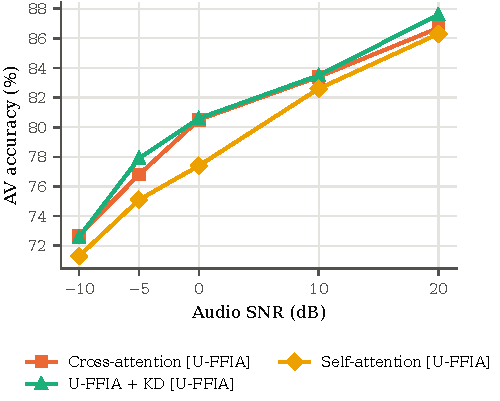
\includegraphics[width=\columnwidth]{figures/robustness_snr.pdf}}{\fbox{\parbox{0.9\columnwidth}{\centering run \texttt{scripts/make\_paper\_assets.py}}}}
  \caption{Audio-visual accuracy as the audio SNR decreases.}
  \label{fig:robust}
\end{figure}

\subsection{Evaluation protocol and data leakage}
\label{sec:protocols}
Table~\ref{tab:protocols} evaluates the same model under the three protocols of Sec.~\ref{sec:setup}:
\resOfficialAcc\,\% on the official split, \resKfoldAcc\,\% under 5-fold CV, and \resGroupedAcc\,\% on
the session-disjoint split.
\todo{If the session-disjoint accuracy is markedly lower, state that clip-level random splits
overestimate generalisation on AV-FFIA, and that published results above 95\% should be read with this
in mind.}

\begin{table}[t]
  \centering
  \caption{One model under three evaluation protocols.}
  \label{tab:protocols}
  \footnotesize
  \resizebox{\columnwidth}{!}{\input{tables/protocols.tex}}
\end{table}

\subsection{Per-class analysis}
\label{sec:perclass}
Table~\ref{tab:perclass} and Fig.~\ref{fig:confusion} give the per-class F1 and the confusion matrix
of HyperAVNet-Q (KD).
\todo{Discuss the dominant confusions, expected between the adjacent intensities Weak and Medium,
and how much the audio stream contributes to separating them.}

\begin{table}[t]
  \centering
  \caption{Per-class F1 of HyperAVNet-Q (KD), official split.}
  \label{tab:perclass}
  \footnotesize
  \input{tables/per_class.tex}
\end{table}

\begin{figure}[t]
  \centering
  \IfFileExists{figures/confusion.pdf}{\includegraphics[width=0.7\columnwidth]{figures/confusion.pdf}}{\fbox{\parbox{0.9\columnwidth}{\centering pending runs}}}
  \caption{Row-normalised confusion matrix (\%) of HyperAVNet-Q (KD), summed over seeds.}
  \label{fig:confusion}
\end{figure}

\subsection{Deployment}
\label{sec:deploy}
Table~\ref{tab:deploy} measures the cost of the two forms of the model on \resDeployDevice{} (batch 1).
In training form, every hypercomplex kernel is assembled from its $n$ blocks at each forward pass.
After reparameterisation (Sec.~\ref{sec:hyper}) the kernels are dense, and latency falls from
\resLatTrain\,ms to \resLatDeploy\,ms. The trade-off is explicit: the hypercomplex form stores and
transmits $n\times$ fewer parameters (2.14\,M), while the deployed dense form holds 7.88\,M parameters
in memory and runs faster. A device can therefore receive the compact model and expand it once at load
time.

\begin{table}[t]
  \centering
  \caption{Training-form versus reparameterised (deployed) model. Stored: parameters kept on disk and
  transmitted; Dense: parameters in memory after reparameterisation.}
  \label{tab:deploy}
  \footnotesize
  \IfFileExists{tables/deploy.tex}{\resizebox{\columnwidth}{!}{\input{tables/deploy.tex}}}{\fbox{run \texttt{profile\_model.py --out}}}
\end{table}

\subsection{Limitations}
\label{sec:limitations}
Hypercomplex layers reduce stored parameters but not arithmetic, so the compute savings come from the
compact backbone design rather than from the algebra. AV-FFIA covers one species and one tank, and
generalisation to farm conditions (turbidity, foam, other species) remains to be shown. Finally, the
discrepancies in the public data release, and the variety of protocols in the literature, limit how
precisely results can be compared across papers.

%  Numbers come from tables/*.tex and tables/macros.tex, generated by
%  scripts/make_paper_assets.py from the run folders. Re-run it after new runs.
%  Sentences marked \todo{} state a claim that must be checked against the
%  final numbers (keep, reverse or delete).
% ============================================================================
\section{Results}
\label{sec:results}

\subsection{Comparison with the state of the art}
\label{sec:main}
Table~\ref{tab:main} lists the published results on AV-FFIA with their protocols, followed by our models
under the official split. The distilled quaternion model, HyperAVNet-Q (KD), reaches
\resOurAcc\,\% accuracy (macro-F1 \resOurFone\,\%) with \resOurParams\,M parameters and
\resOurGMACs\,GMACs per clip. That is 10.1$\times$ fewer parameters and 13.1$\times$ fewer MACs than
U-FFIA~\cite{cui2024uffia}, and 16.4$\times$ / 51.6$\times$ fewer than the cross-attention model.
\todo{Position against the strongest comparable result: DynaGate-AV reports 96.4--96.5\% on the same
official split rule, and HMMF-Net 96.77\% under 5-fold CV (Table~\ref{tab:protocols}). State whether
HyperAVNet exceeds, matches or trails them; LDMF and HMKD use filtered subsets and are not comparable.}
Fig.~\ref{fig:acc_compute} places all models on an accuracy--compute plane.
Its single-modality heads reach \resOurAccA\,\% (audio) and \resOurAccV\,\% (video), against the
best published single-modality models, Pre-CNN10 (85.9\%) and Pretrained-S3D (89.8\%)~\cite{cui2024uffia}.

\begin{table*}[t]
  \centering
  \caption{Comparison on AV-FFIA. Compute is in GMACs per 2\,s clip; U-FFIA's ``FLOPs'' are MACs.
  Published numbers are quoted with their own protocol and are not directly comparable across
  protocols. $^\dagger$Not verified against the full paper (taken from secondary sources). Our
  rows: official split, mean $\pm$ std over three seeds.}
  \label{tab:main}
  \small
  \resizebox{\textwidth}{!}{\begin{tabular}{llrrrrl}
\toprule
Method & Mod. & Params (M) & GMACs & Acc. (\%) & F1 (\%) & Protocol \\
\midrule
Pre-CNN10~\cite{cui2024uffia} & A & 5.00 & 3.347 & 85.9 & -- & paper split \\
Pretrained-S3D~\cite{cui2024uffia} & V & 7.90 & 22.826 & 89.8 & -- & paper split \\
Self-attention~\cite{cui2024uffia} & AV & 47.70 & 68.404 & 89.2 & -- & paper split \\
MBT~\cite{cui2024uffia} & AV & 47.69 & 68.690 & 72.4 & -- & paper split \\
Cross-attention~\cite{cui2024uffia} & AV & 35.08 & 60.933 & 91.7 & -- & paper split \\
U-FFIA + KD~\cite{cui2024uffia} & AV & 21.63 & 15.488 & 90.7 & -- & paper split \\
\midrule
ACAF-Net~\cite{acafnet2025}$^\dagger$ & AV & -- & -- & 95.4 & -- & random split \\
DynaGate-AV (Light)~\cite{dynagate2026} & AV & -- & 5.290 & 96.4 & -- & official split, 19,963 clips \\
HMMF-Net~\cite{hmmfnet2026}$^\dagger$ & AV & 3.99 & 1.002 & 96.8 & 96.9 & 5-fold CV \\
HMKD~\cite{hmkd2026}$^\dagger$ & AV & -- & -- & 97.5 & -- & 26,843-pair holdout \\
LDMF~\cite{ldmf2026}$^\dagger$ & AV & 7.10 & -- & 98.2 & -- & filtered subset \\
\midrule
Real late-concat baseline (ours, re-run) & AV & -- & -- & -- & -- & official split \\
Teacher: CNN10 + S3D + HCF & AV & -- & -- & -- & -- & official split \\
Teacher: EfficientAT + MoViNet-A0 + HCF & AV & -- & -- & -- & -- & official split \\
HyperAVNet-Q (no KD) & AV & -- & -- & -- & -- & official split \\
\textbf{HyperAVNet-Q (KD)} & AV & -- & -- & -- & -- & official split \\
HyperAVNet-P (pretrained, no KD) & AV & -- & -- & -- & -- & official split \\
HyperAVNet-P (pretrained, KD) & AV & -- & -- & -- & -- & official split \\
HyperAVNet-O (KD) & AV & -- & -- & -- & -- & official split \\
\bottomrule
\end{tabular}
}
\end{table*}

\begin{figure}[t]
  \centering
  \IfFileExists{figures/acc_vs_compute.pdf}{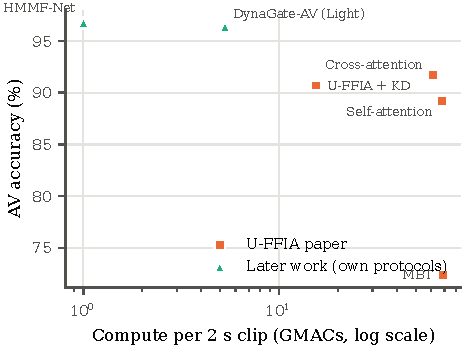
\includegraphics[width=\columnwidth]{figures/acc_vs_compute.pdf}}{\fbox{\parbox{0.9\columnwidth}{\centering run \texttt{scripts/make\_paper\_assets.py}}}}
  \caption{Accuracy versus compute (log scale) on AV-FFIA. Published models are plotted at their
  reported values and protocols; HyperAVNet uses the official split.}
  \label{fig:acc_compute}
\end{figure}

\subsection{Where to fuse: the deep-to-early study}
\label{sec:depth}
Table~\ref{tab:depth} and Fig.~\ref{fig:depth} vary the fusion set $\mathcal{S}$. Late fusion
($\mathcal{S}=\{3\}$) gives \resLateAcc\,\%; progressive fusion from stage~1 gives \resProgAcc\,\%;
the best setting is $\mathcal{S}=\resBestDepth$. Fusion is nearly free in compute: each additional HCF
stage costs about 0.17\,M parameters and under 0.02\,GMACs. Disabling the cross-modal feedback of
Eq.~\eqref{eq:feedback} at $\mathcal{S}=\{1,2,3\}$ gives \resNoFeedbackAcc\,\%.
\todo{Interpret: does accuracy grow as fusion moves earlier, saturate, or peak at mid-level stages
(an inverted U)? Does feedback help, and does the gain concentrate on Weak and Medium? Use the
single-stage rows to locate the most useful depth.}

\begin{table}[t]
  \centering
  \caption{Fusion depth (deep to early) and cross-modal feedback. Mean $\pm$ std, official split.}
  \label{tab:depth}
  \footnotesize
  \setlength{\tabcolsep}{3pt}
  \resizebox{\columnwidth}{!}{\begin{tabular}{lrrrrrr}
\toprule
Fusion stages $\mathcal{S}$ & Params (M) & GMACs & Acc. & F1 & A-only & V-only \\
\midrule
$\{3\}$ (late) & -- & -- & -- & -- & -- & -- \\
$\{2,3\}$ & -- & -- & -- & -- & -- & -- \\
$\{1,2,3\}$ & -- & -- & -- & -- & -- & -- \\
$\{0,1,2,3\}$ & -- & -- & -- & -- & -- & -- \\
\midrule
$\{0\}$ & -- & -- & -- & -- & -- & -- \\
$\{1\}$ & -- & -- & -- & -- & -- & -- \\
$\{2\}$ & -- & -- & -- & -- & -- & -- \\
\midrule
$\{1,2,3\}$ w/o feedback & -- & -- & -- & -- & -- & -- \\
\bottomrule
\end{tabular}
}
\end{table}

\begin{figure}[t]
  \centering
  \IfFileExists{figures/fusion_depth.pdf}{\includegraphics[width=\columnwidth]{figures/fusion_depth.pdf}}{\fbox{\parbox{0.9\columnwidth}{\centering pending runs \texttt{A\_fs*}}}}
  \caption{Accuracy as fusion moves from the last stage to all stages, with and without feedback.}
  \label{fig:depth}
\end{figure}

\subsection{Effect of the hypercomplex algebra}
\label{sec:algebra}
Table~\ref{tab:algebra} and Fig.~\ref{fig:algebra} replace every hypercomplex layer of the network with
algebra $\mathbb{A}_n$. All variants share the architecture and compute and differ only in weight
sharing. The real network ($n=1$, 7.88\,M parameters) reaches \resRealAcc\,\%, the quaternion network
(2.14\,M) \resQuatAcc\,\% and the octonion network (1.24\,M) \resOctAcc\,\%.
\todo{Interpret: if accuracy is maintained or improved down to $n=4$ or $n=8$, the Hamilton
weight sharing acts as a useful structural prior on a dataset of this size; report where accuracy
starts to drop.}

\begin{table}[t]
  \centering
  \caption{Algebra of the whole network. Compute is identical for all $n$.}
  \label{tab:algebra}
  \footnotesize
  \resizebox{\columnwidth}{!}{\begin{tabular}{lrrrr}
\toprule
Algebra & Params (M) & GMACs & Acc. & F1 \\
\midrule
Real ($n{=}1$) & -- & -- & -- & -- \\
Complex ($n{=}2$) & -- & -- & -- & -- \\
Quaternion ($n{=}4$) & -- & -- & -- & -- \\
Octonion ($n{=}8$) & -- & -- & -- & -- \\
Sedenion ($n{=}16$) & -- & -- & -- & -- \\
\bottomrule
\end{tabular}
}
\end{table}

\begin{figure}[t]
  \centering
  \IfFileExists{figures/algebra.pdf}{\includegraphics[width=\columnwidth]{figures/algebra.pdf}}{\fbox{\parbox{0.9\columnwidth}{\centering pending runs \texttt{B\_n*}}}}
  \caption{Accuracy against parameter count for real, complex, quaternion, octonion and sedenion networks.}
  \label{fig:algebra}
\end{figure}

\subsection{Fusion operator, regularisers and front-end}
\label{sec:operators}
Table~\ref{tab:ops} compares HCF with a hypercomplex attention bottleneck (MBT) at equal parameters,
and with gated concatenation. HCF with quaternion components gives \resHCFAcc\,\% and MBT
\resMBTAcc\,\%. In~\cite{cui2024uffia}, MBT also trailed cross-attention by a wide margin
(72.4\% vs.\ 91.7\%), which the authors attributed to attending to the modalities one after the other.
\todo{State whether parallel reading plus Hamilton mixing closes this gap, and whether octonion
components (four extra interaction terms, same parameters) help.}
The lower block of Table~\ref{tab:ops} isolates modality dropout, the auxiliary heads and the SimPF
front-end~\cite{liu2023simpf}.

\begin{table}[t]
  \centering
  \caption{Fusion operator (top), regularisers (middle) and audio front-end (bottom).}
  \label{tab:ops}
  \footnotesize
  \setlength{\tabcolsep}{3pt}
  \resizebox{\columnwidth}{!}{\begin{tabular}{lrrrrr}
\toprule
Variant & Params (M) & Acc. & F1 & A-only & V-only \\
\midrule
HCF, complex components & -- & -- & -- & -- & -- \\
HCF, quaternion components & -- & -- & -- & -- & -- \\
HCF, octonion components & -- & -- & -- & -- & -- \\
Hypercomplex MBT & -- & -- & -- & -- & -- \\
Gated concatenation & -- & -- & -- & -- & -- \\
\midrule
w/o modality dropout ($p{=}0$) & -- & -- & -- & -- & -- \\
modality dropout $p{=}0.25$ & -- & -- & -- & -- & -- \\
w/o auxiliary heads & -- & -- & -- & -- & -- \\
\midrule
SimPF front-end ($k{=}0.5$) & -- & -- & -- & -- & -- \\
\bottomrule
\end{tabular}
}
\end{table}

\subsection{Which teacher? Teacher ablation}
\label{sec:teachers}
Table~\ref{tab:teachers} reports each teacher's audio-visual and unimodal accuracy, and the accuracy
of the student distilled from it; $\Delta$ is student minus teacher. Fig.~\ref{fig:teachers} plots
student against teacher accuracy. Distillation from the default teacher (CNN10 + S3D,
\resTeacherAcc\,\%) changes the student's accuracy by \resKDGain\ points over the same student trained
without a teacher (\resNoKDAcc\,\%).
\todo{Interpret: does a stronger teacher yield a stronger student, or does the compact HMKD pair (T10,
about 1\,GMAC) distil as well as the larger teachers? Do the transformer teachers (T6, T8, T9) under-perform
on AV-FFIA, as AST and ViViT did in~\cite{cui2024uffia}?}

\begin{table*}[t]
  \centering
  \caption{Teacher ablation. Teacher params (M) and GMACs include the HCF fusion network. Student:
  HyperAVNet-Q distilled from that teacher. $\Delta$ = student $-$ teacher accuracy.}
  \label{tab:teachers}
  \small
  \resizebox{\textwidth}{!}{\begin{tabular}{llrrrrrrr}
\toprule
ID & Audio / video teacher & Params & GMACs & Teacher AV & A-only & V-only & Student & $\Delta$ \\
\midrule
T1 & CNN10 / S3D & -- & -- & -- & -- & -- & -- & -- \\
T2 & CNN14 / S3D & -- & -- & -- & -- & -- & -- & -- \\
T3 & CNN10 / R(2+1)D-18 & -- & -- & -- & -- & -- & -- & -- \\
T4 & CNN10 / ConvNeXt-T (frames) & -- & -- & -- & -- & -- & -- & -- \\
T5 & EffNet-B0 (mel) / S3D & -- & -- & -- & -- & -- & -- & -- \\
T6 & AST / VideoMAE-B & -- & -- & -- & -- & -- & -- & -- \\
T7 & CNN10 / X3D-M & -- & -- & -- & -- & -- & -- & -- \\
T8 & AST / S3D & -- & -- & -- & -- & -- & -- & -- \\
T9 & CNN10 / VideoMAE-B & -- & -- & -- & -- & -- & -- & -- \\
T10 & EfficientAT / MoViNet-A0 & -- & -- & -- & -- & -- & -- & -- \\
\midrule
-- & no teacher (no KD) & -- & -- & -- & -- & -- & -- & -- \\
\bottomrule
\end{tabular}
}
\end{table*}

\begin{figure}[t]
  \centering
  \IfFileExists{figures/teacher_student.pdf}{\includegraphics[width=\columnwidth]{figures/teacher_student.pdf}}{\fbox{\parbox{0.9\columnwidth}{\centering pending teacher runs}}}
  \caption{Teacher accuracy against the accuracy of the student distilled from it (dashed: no distillation).}
  \label{fig:teachers}
\end{figure}

\subsection{Robustness to noise and missing modalities}
\label{sec:robustness}
Table~\ref{tab:robust} and Fig.~\ref{fig:robust} follow the robustness protocol of~\cite{cui2024uffia}.
\todo{Compare the degradation at $-10$\,dB with U-FFIA (90.7\%$\to$72.6\%) and cross-attention
(91.7\%$\to$72.7\%), only if the same bubble and pump noise was used; otherwise describe the results
as indicative. Discuss the missing-modality columns: the auxiliary heads and masked training should
keep useful accuracy when one modality is absent.}

\begin{table*}[t]
  \centering
  \caption{Robustness. Audio noise at the given SNR (U-FFIA protocol); Dark: video intensities
  $\times0.25$; Noise: Gaussian video noise, $\sigma^{2}=0.2$; $-$A / $-$V: audio / video absent.
  Published rows from~\cite{cui2024uffia} (bubble and pump noise).}
  \label{tab:robust}
  \small
  \resizebox{\textwidth}{!}{\begin{tabular}{lrrrrrrrrrr}
\toprule
Method & Clean & -10\,dB & -5\,dB & +0\,dB & +10\,dB & +20\,dB & Dark & Noise & $-$A & $-$V \\
\midrule
Cross-attention~\cite{cui2024uffia} & 91.7 & 72.7 & 76.8 & 80.5 & 83.4 & 86.7 & -- & -- & -- & -- \\
U-FFIA + KD~\cite{cui2024uffia} & 90.7 & 72.6 & 77.9 & 80.6 & 83.5 & 87.6 & -- & -- & -- & -- \\
Self-attention~\cite{cui2024uffia} & 89.2 & 71.3 & 75.1 & 77.4 & 82.6 & 86.3 & -- & -- & -- & -- \\
\midrule
Teacher (CNN10 + S3D) & -- & -- & -- & -- & -- & -- & -- & -- & -- & -- \\
\textbf{HyperAVNet-Q (KD)} & -- & -- & -- & -- & -- & -- & -- & -- & -- & -- \\
\bottomrule
\end{tabular}
}
\end{table*}

\begin{figure}[t]
  \centering
  \IfFileExists{figures/robustness_snr.pdf}{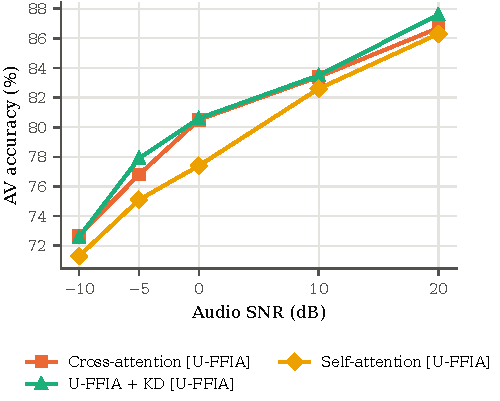
\includegraphics[width=\columnwidth]{figures/robustness_snr.pdf}}{\fbox{\parbox{0.9\columnwidth}{\centering run \texttt{scripts/make\_paper\_assets.py}}}}
  \caption{Audio-visual accuracy as the audio SNR decreases.}
  \label{fig:robust}
\end{figure}

\subsection{Evaluation protocol and data leakage}
\label{sec:protocols}
Table~\ref{tab:protocols} evaluates the same model under the three protocols of Sec.~\ref{sec:setup}:
\resOfficialAcc\,\% on the official split, \resKfoldAcc\,\% under 5-fold CV, and \resGroupedAcc\,\% on
the session-disjoint split.
\todo{If the session-disjoint accuracy is markedly lower, state that clip-level random splits
overestimate generalisation on AV-FFIA, and that published results above 95\% should be read with this
in mind.}

\begin{table}[t]
  \centering
  \caption{One model under three evaluation protocols.}
  \label{tab:protocols}
  \footnotesize
  \resizebox{\columnwidth}{!}{\begin{tabular}{lrrr}
\toprule
Evaluation protocol & Runs & Acc. & F1 \\
\midrule
Official code split (700/700 per class) & -- & -- & -- \\
5-fold stratified CV & -- & -- & -- \\
Session-disjoint (whole recording dates) & -- & -- & -- \\
\bottomrule
\end{tabular}
}
\end{table}

\subsection{Per-class analysis}
\label{sec:perclass}
Table~\ref{tab:perclass} and Fig.~\ref{fig:confusion} give the per-class F1 and the confusion matrix
of HyperAVNet-Q (KD).
\todo{Discuss the dominant confusions, expected between the adjacent intensities Weak and Medium,
and how much the audio stream contributes to separating them.}

\begin{table}[t]
  \centering
  \caption{Per-class F1 of HyperAVNet-Q (KD), official split.}
  \label{tab:perclass}
  \footnotesize
  \begin{tabular}{lr}
\toprule
Class & F1 (\%) \\
\midrule
None & -- \\
Strong & -- \\
Medium & -- \\
Weak & -- \\
\bottomrule
\end{tabular}

\end{table}

\begin{figure}[t]
  \centering
  \IfFileExists{figures/confusion.pdf}{\includegraphics[width=0.7\columnwidth]{figures/confusion.pdf}}{\fbox{\parbox{0.9\columnwidth}{\centering pending runs}}}
  \caption{Row-normalised confusion matrix (\%) of HyperAVNet-Q (KD), summed over seeds.}
  \label{fig:confusion}
\end{figure}

\subsection{Deployment}
\label{sec:deploy}
Table~\ref{tab:deploy} measures the cost of the two forms of the model on \resDeployDevice{} (batch 1).
In training form, every hypercomplex kernel is assembled from its $n$ blocks at each forward pass.
After reparameterisation (Sec.~\ref{sec:hyper}) the kernels are dense, and latency falls from
\resLatTrain\,ms to \resLatDeploy\,ms. The trade-off is explicit: the hypercomplex form stores and
transmits $n\times$ fewer parameters (2.14\,M), while the deployed dense form holds 7.88\,M parameters
in memory and runs faster. A device can therefore receive the compact model and expand it once at load
time.

\begin{table}[t]
  \centering
  \caption{Training-form versus reparameterised (deployed) model. Stored: parameters kept on disk and
  transmitted; Dense: parameters in memory after reparameterisation.}
  \label{tab:deploy}
  \footnotesize
  \IfFileExists{tables/deploy.tex}{\resizebox{\columnwidth}{!}{\begin{tabular}{lrrrrrr}
\toprule
Model & Stored (M) & Dense (M) & GMACs & Train-form (ms) & Deployed (ms) & Speed-up \\
\midrule
-- & -- & -- & -- & -- & -- & -- \\
\bottomrule
\end{tabular}
}}{\fbox{run \texttt{profile\_model.py --out}}}
\end{table}

\subsection{Limitations}
\label{sec:limitations}
Hypercomplex layers reduce stored parameters but not arithmetic, so the compute savings come from the
compact backbone design rather than from the algebra. AV-FFIA covers one species and one tank, and
generalisation to farm conditions (turbidity, foam, other species) remains to be shown. Finally, the
discrepancies in the public data release, and the variety of protocols in the literature, limit how
precisely results can be compared across papers.

%  Numbers come from tables/*.tex and tables/macros.tex, generated by
%  scripts/make_paper_assets.py from the run folders. Re-run it after new runs.
%  Sentences marked \todo{} state a claim that must be checked against the
%  final numbers (keep, reverse or delete).
% ============================================================================
\section{Results}
\label{sec:results}

\subsection{Comparison with the state of the art}
\label{sec:main}
Table~\ref{tab:main} lists the published results on AV-FFIA with their protocols, followed by our models
under the official split. The distilled quaternion model, HyperAVNet-Q (KD), reaches
\resOurAcc\,\% accuracy (macro-F1 \resOurFone\,\%) with \resOurParams\,M parameters and
\resOurGMACs\,GMACs per clip. That is 10.1$\times$ fewer parameters and 13.1$\times$ fewer MACs than
U-FFIA~\cite{cui2024uffia}, and 16.4$\times$ / 51.6$\times$ fewer than the cross-attention model.
\todo{Position against the strongest comparable result: DynaGate-AV reports 96.4--96.5\% on the same
official split rule, and HMMF-Net 96.77\% under 5-fold CV (Table~\ref{tab:protocols}). State whether
HyperAVNet exceeds, matches or trails them; LDMF and HMKD use filtered subsets and are not comparable.}
Fig.~\ref{fig:acc_compute} places all models on an accuracy--compute plane.
Its single-modality heads reach \resOurAccA\,\% (audio) and \resOurAccV\,\% (video), against the
best published single-modality models, Pre-CNN10 (85.9\%) and Pretrained-S3D (89.8\%)~\cite{cui2024uffia}.

\begin{table*}[t]
  \centering
  \caption{Comparison on AV-FFIA. Compute is in GMACs per 2\,s clip; U-FFIA's ``FLOPs'' are MACs.
  Published numbers are quoted with their own protocol and are not directly comparable across
  protocols. $^\dagger$Not verified against the full paper (taken from secondary sources). Our
  rows: official split, mean $\pm$ std over three seeds.}
  \label{tab:main}
  \small
  \resizebox{\textwidth}{!}{\begin{tabular}{llrrrrl}
\toprule
Method & Mod. & Params (M) & GMACs & Acc. (\%) & F1 (\%) & Protocol \\
\midrule
Pre-CNN10~\cite{cui2024uffia} & A & 5.00 & 3.347 & 85.9 & -- & paper split \\
Pretrained-S3D~\cite{cui2024uffia} & V & 7.90 & 22.826 & 89.8 & -- & paper split \\
Self-attention~\cite{cui2024uffia} & AV & 47.70 & 68.404 & 89.2 & -- & paper split \\
MBT~\cite{cui2024uffia} & AV & 47.69 & 68.690 & 72.4 & -- & paper split \\
Cross-attention~\cite{cui2024uffia} & AV & 35.08 & 60.933 & 91.7 & -- & paper split \\
U-FFIA + KD~\cite{cui2024uffia} & AV & 21.63 & 15.488 & 90.7 & -- & paper split \\
\midrule
ACAF-Net~\cite{acafnet2025}$^\dagger$ & AV & -- & -- & 95.4 & -- & random split \\
DynaGate-AV (Light)~\cite{dynagate2026} & AV & -- & 5.290 & 96.4 & -- & official split, 19,963 clips \\
HMMF-Net~\cite{hmmfnet2026}$^\dagger$ & AV & 3.99 & 1.002 & 96.8 & 96.9 & 5-fold CV \\
HMKD~\cite{hmkd2026}$^\dagger$ & AV & -- & -- & 97.5 & -- & 26,843-pair holdout \\
LDMF~\cite{ldmf2026}$^\dagger$ & AV & 7.10 & -- & 98.2 & -- & filtered subset \\
\midrule
Real late-concat baseline (ours, re-run) & AV & -- & -- & -- & -- & official split \\
Teacher: CNN10 + S3D + HCF & AV & -- & -- & -- & -- & official split \\
Teacher: EfficientAT + MoViNet-A0 + HCF & AV & -- & -- & -- & -- & official split \\
HyperAVNet-Q (no KD) & AV & -- & -- & -- & -- & official split \\
\textbf{HyperAVNet-Q (KD)} & AV & -- & -- & -- & -- & official split \\
HyperAVNet-P (pretrained, no KD) & AV & -- & -- & -- & -- & official split \\
HyperAVNet-P (pretrained, KD) & AV & -- & -- & -- & -- & official split \\
HyperAVNet-O (KD) & AV & -- & -- & -- & -- & official split \\
\bottomrule
\end{tabular}
}
\end{table*}

\begin{figure}[t]
  \centering
  \IfFileExists{figures/acc_vs_compute.pdf}{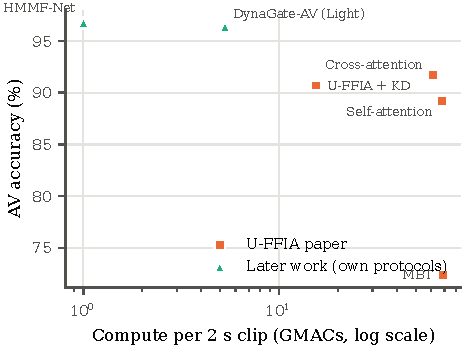
\includegraphics[width=\columnwidth]{figures/acc_vs_compute.pdf}}{\fbox{\parbox{0.9\columnwidth}{\centering run \texttt{scripts/make\_paper\_assets.py}}}}
  \caption{Accuracy versus compute (log scale) on AV-FFIA. Published models are plotted at their
  reported values and protocols; HyperAVNet uses the official split.}
  \label{fig:acc_compute}
\end{figure}

\subsection{Where to fuse: the deep-to-early study}
\label{sec:depth}
Table~\ref{tab:depth} and Fig.~\ref{fig:depth} vary the fusion set $\mathcal{S}$. Late fusion
($\mathcal{S}=\{3\}$) gives \resLateAcc\,\%; progressive fusion from stage~1 gives \resProgAcc\,\%;
the best setting is $\mathcal{S}=\resBestDepth$. Fusion is nearly free in compute: each additional HCF
stage costs about 0.17\,M parameters and under 0.02\,GMACs. Disabling the cross-modal feedback of
Eq.~\eqref{eq:feedback} at $\mathcal{S}=\{1,2,3\}$ gives \resNoFeedbackAcc\,\%.
\todo{Interpret: does accuracy grow as fusion moves earlier, saturate, or peak at mid-level stages
(an inverted U)? Does feedback help, and does the gain concentrate on Weak and Medium? Use the
single-stage rows to locate the most useful depth.}

\begin{table}[t]
  \centering
  \caption{Fusion depth (deep to early) and cross-modal feedback. Mean $\pm$ std, official split.}
  \label{tab:depth}
  \footnotesize
  \setlength{\tabcolsep}{3pt}
  \resizebox{\columnwidth}{!}{\begin{tabular}{lrrrrrr}
\toprule
Fusion stages $\mathcal{S}$ & Params (M) & GMACs & Acc. & F1 & A-only & V-only \\
\midrule
$\{3\}$ (late) & -- & -- & -- & -- & -- & -- \\
$\{2,3\}$ & -- & -- & -- & -- & -- & -- \\
$\{1,2,3\}$ & -- & -- & -- & -- & -- & -- \\
$\{0,1,2,3\}$ & -- & -- & -- & -- & -- & -- \\
\midrule
$\{0\}$ & -- & -- & -- & -- & -- & -- \\
$\{1\}$ & -- & -- & -- & -- & -- & -- \\
$\{2\}$ & -- & -- & -- & -- & -- & -- \\
\midrule
$\{1,2,3\}$ w/o feedback & -- & -- & -- & -- & -- & -- \\
\bottomrule
\end{tabular}
}
\end{table}

\begin{figure}[t]
  \centering
  \IfFileExists{figures/fusion_depth.pdf}{\includegraphics[width=\columnwidth]{figures/fusion_depth.pdf}}{\fbox{\parbox{0.9\columnwidth}{\centering pending runs \texttt{A\_fs*}}}}
  \caption{Accuracy as fusion moves from the last stage to all stages, with and without feedback.}
  \label{fig:depth}
\end{figure}

\subsection{Effect of the hypercomplex algebra}
\label{sec:algebra}
Table~\ref{tab:algebra} and Fig.~\ref{fig:algebra} replace every hypercomplex layer of the network with
algebra $\mathbb{A}_n$. All variants share the architecture and compute and differ only in weight
sharing. The real network ($n=1$, 7.88\,M parameters) reaches \resRealAcc\,\%, the quaternion network
(2.14\,M) \resQuatAcc\,\% and the octonion network (1.24\,M) \resOctAcc\,\%.
\todo{Interpret: if accuracy is maintained or improved down to $n=4$ or $n=8$, the Hamilton
weight sharing acts as a useful structural prior on a dataset of this size; report where accuracy
starts to drop.}

\begin{table}[t]
  \centering
  \caption{Algebra of the whole network. Compute is identical for all $n$.}
  \label{tab:algebra}
  \footnotesize
  \resizebox{\columnwidth}{!}{\begin{tabular}{lrrrr}
\toprule
Algebra & Params (M) & GMACs & Acc. & F1 \\
\midrule
Real ($n{=}1$) & -- & -- & -- & -- \\
Complex ($n{=}2$) & -- & -- & -- & -- \\
Quaternion ($n{=}4$) & -- & -- & -- & -- \\
Octonion ($n{=}8$) & -- & -- & -- & -- \\
Sedenion ($n{=}16$) & -- & -- & -- & -- \\
\bottomrule
\end{tabular}
}
\end{table}

\begin{figure}[t]
  \centering
  \IfFileExists{figures/algebra.pdf}{\includegraphics[width=\columnwidth]{figures/algebra.pdf}}{\fbox{\parbox{0.9\columnwidth}{\centering pending runs \texttt{B\_n*}}}}
  \caption{Accuracy against parameter count for real, complex, quaternion, octonion and sedenion networks.}
  \label{fig:algebra}
\end{figure}

\subsection{Fusion operator, regularisers and front-end}
\label{sec:operators}
Table~\ref{tab:ops} compares HCF with a hypercomplex attention bottleneck (MBT) at equal parameters,
and with gated concatenation. HCF with quaternion components gives \resHCFAcc\,\% and MBT
\resMBTAcc\,\%. In~\cite{cui2024uffia}, MBT also trailed cross-attention by a wide margin
(72.4\% vs.\ 91.7\%), which the authors attributed to attending to the modalities one after the other.
\todo{State whether parallel reading plus Hamilton mixing closes this gap, and whether octonion
components (four extra interaction terms, same parameters) help.}
The lower block of Table~\ref{tab:ops} isolates modality dropout, the auxiliary heads and the SimPF
front-end~\cite{liu2023simpf}.

\begin{table}[t]
  \centering
  \caption{Fusion operator (top), regularisers (middle) and audio front-end (bottom).}
  \label{tab:ops}
  \footnotesize
  \setlength{\tabcolsep}{3pt}
  \resizebox{\columnwidth}{!}{\begin{tabular}{lrrrrr}
\toprule
Variant & Params (M) & Acc. & F1 & A-only & V-only \\
\midrule
HCF, complex components & -- & -- & -- & -- & -- \\
HCF, quaternion components & -- & -- & -- & -- & -- \\
HCF, octonion components & -- & -- & -- & -- & -- \\
Hypercomplex MBT & -- & -- & -- & -- & -- \\
Gated concatenation & -- & -- & -- & -- & -- \\
\midrule
w/o modality dropout ($p{=}0$) & -- & -- & -- & -- & -- \\
modality dropout $p{=}0.25$ & -- & -- & -- & -- & -- \\
w/o auxiliary heads & -- & -- & -- & -- & -- \\
\midrule
SimPF front-end ($k{=}0.5$) & -- & -- & -- & -- & -- \\
\bottomrule
\end{tabular}
}
\end{table}

\subsection{Which teacher? Teacher ablation}
\label{sec:teachers}
Table~\ref{tab:teachers} reports each teacher's audio-visual and unimodal accuracy, and the accuracy
of the student distilled from it; $\Delta$ is student minus teacher. Fig.~\ref{fig:teachers} plots
student against teacher accuracy. Distillation from the default teacher (CNN10 + S3D,
\resTeacherAcc\,\%) changes the student's accuracy by \resKDGain\ points over the same student trained
without a teacher (\resNoKDAcc\,\%).
\todo{Interpret: does a stronger teacher yield a stronger student, or does the compact HMKD pair (T10,
about 1\,GMAC) distil as well as the larger teachers? Do the transformer teachers (T6, T8, T9) under-perform
on AV-FFIA, as AST and ViViT did in~\cite{cui2024uffia}?}

\begin{table*}[t]
  \centering
  \caption{Teacher ablation. Teacher params (M) and GMACs include the HCF fusion network. Student:
  HyperAVNet-Q distilled from that teacher. $\Delta$ = student $-$ teacher accuracy.}
  \label{tab:teachers}
  \small
  \resizebox{\textwidth}{!}{\begin{tabular}{llrrrrrrr}
\toprule
ID & Audio / video teacher & Params & GMACs & Teacher AV & A-only & V-only & Student & $\Delta$ \\
\midrule
T1 & CNN10 / S3D & -- & -- & -- & -- & -- & -- & -- \\
T2 & CNN14 / S3D & -- & -- & -- & -- & -- & -- & -- \\
T3 & CNN10 / R(2+1)D-18 & -- & -- & -- & -- & -- & -- & -- \\
T4 & CNN10 / ConvNeXt-T (frames) & -- & -- & -- & -- & -- & -- & -- \\
T5 & EffNet-B0 (mel) / S3D & -- & -- & -- & -- & -- & -- & -- \\
T6 & AST / VideoMAE-B & -- & -- & -- & -- & -- & -- & -- \\
T7 & CNN10 / X3D-M & -- & -- & -- & -- & -- & -- & -- \\
T8 & AST / S3D & -- & -- & -- & -- & -- & -- & -- \\
T9 & CNN10 / VideoMAE-B & -- & -- & -- & -- & -- & -- & -- \\
T10 & EfficientAT / MoViNet-A0 & -- & -- & -- & -- & -- & -- & -- \\
\midrule
-- & no teacher (no KD) & -- & -- & -- & -- & -- & -- & -- \\
\bottomrule
\end{tabular}
}
\end{table*}

\begin{figure}[t]
  \centering
  \IfFileExists{figures/teacher_student.pdf}{\includegraphics[width=\columnwidth]{figures/teacher_student.pdf}}{\fbox{\parbox{0.9\columnwidth}{\centering pending teacher runs}}}
  \caption{Teacher accuracy against the accuracy of the student distilled from it (dashed: no distillation).}
  \label{fig:teachers}
\end{figure}

\subsection{Robustness to noise and missing modalities}
\label{sec:robustness}
Table~\ref{tab:robust} and Fig.~\ref{fig:robust} follow the robustness protocol of~\cite{cui2024uffia}.
\todo{Compare the degradation at $-10$\,dB with U-FFIA (90.7\%$\to$72.6\%) and cross-attention
(91.7\%$\to$72.7\%), only if the same bubble and pump noise was used; otherwise describe the results
as indicative. Discuss the missing-modality columns: the auxiliary heads and masked training should
keep useful accuracy when one modality is absent.}

\begin{table*}[t]
  \centering
  \caption{Robustness. Audio noise at the given SNR (U-FFIA protocol); Dark: video intensities
  $\times0.25$; Noise: Gaussian video noise, $\sigma^{2}=0.2$; $-$A / $-$V: audio / video absent.
  Published rows from~\cite{cui2024uffia} (bubble and pump noise).}
  \label{tab:robust}
  \small
  \resizebox{\textwidth}{!}{\begin{tabular}{lrrrrrrrrrr}
\toprule
Method & Clean & -10\,dB & -5\,dB & +0\,dB & +10\,dB & +20\,dB & Dark & Noise & $-$A & $-$V \\
\midrule
Cross-attention~\cite{cui2024uffia} & 91.7 & 72.7 & 76.8 & 80.5 & 83.4 & 86.7 & -- & -- & -- & -- \\
U-FFIA + KD~\cite{cui2024uffia} & 90.7 & 72.6 & 77.9 & 80.6 & 83.5 & 87.6 & -- & -- & -- & -- \\
Self-attention~\cite{cui2024uffia} & 89.2 & 71.3 & 75.1 & 77.4 & 82.6 & 86.3 & -- & -- & -- & -- \\
\midrule
Teacher (CNN10 + S3D) & -- & -- & -- & -- & -- & -- & -- & -- & -- & -- \\
\textbf{HyperAVNet-Q (KD)} & -- & -- & -- & -- & -- & -- & -- & -- & -- & -- \\
\bottomrule
\end{tabular}
}
\end{table*}

\begin{figure}[t]
  \centering
  \IfFileExists{figures/robustness_snr.pdf}{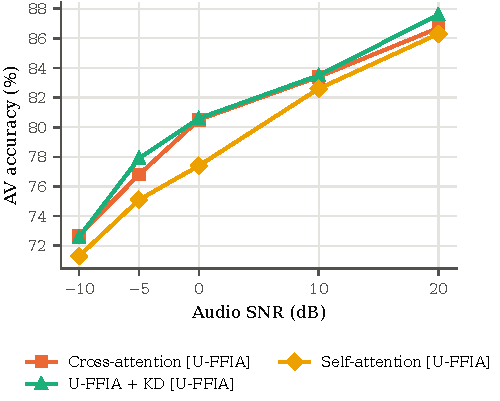
\includegraphics[width=\columnwidth]{figures/robustness_snr.pdf}}{\fbox{\parbox{0.9\columnwidth}{\centering run \texttt{scripts/make\_paper\_assets.py}}}}
  \caption{Audio-visual accuracy as the audio SNR decreases.}
  \label{fig:robust}
\end{figure}

\subsection{Evaluation protocol and data leakage}
\label{sec:protocols}
Table~\ref{tab:protocols} evaluates the same model under the three protocols of Sec.~\ref{sec:setup}:
\resOfficialAcc\,\% on the official split, \resKfoldAcc\,\% under 5-fold CV, and \resGroupedAcc\,\% on
the session-disjoint split.
\todo{If the session-disjoint accuracy is markedly lower, state that clip-level random splits
overestimate generalisation on AV-FFIA, and that published results above 95\% should be read with this
in mind.}

\begin{table}[t]
  \centering
  \caption{One model under three evaluation protocols.}
  \label{tab:protocols}
  \footnotesize
  \resizebox{\columnwidth}{!}{\begin{tabular}{lrrr}
\toprule
Evaluation protocol & Runs & Acc. & F1 \\
\midrule
Official code split (700/700 per class) & -- & -- & -- \\
5-fold stratified CV & -- & -- & -- \\
Session-disjoint (whole recording dates) & -- & -- & -- \\
\bottomrule
\end{tabular}
}
\end{table}

\subsection{Per-class analysis}
\label{sec:perclass}
Table~\ref{tab:perclass} and Fig.~\ref{fig:confusion} give the per-class F1 and the confusion matrix
of HyperAVNet-Q (KD).
\todo{Discuss the dominant confusions, expected between the adjacent intensities Weak and Medium,
and how much the audio stream contributes to separating them.}

\begin{table}[t]
  \centering
  \caption{Per-class F1 of HyperAVNet-Q (KD), official split.}
  \label{tab:perclass}
  \footnotesize
  \begin{tabular}{lr}
\toprule
Class & F1 (\%) \\
\midrule
None & -- \\
Strong & -- \\
Medium & -- \\
Weak & -- \\
\bottomrule
\end{tabular}

\end{table}

\begin{figure}[t]
  \centering
  \IfFileExists{figures/confusion.pdf}{\includegraphics[width=0.7\columnwidth]{figures/confusion.pdf}}{\fbox{\parbox{0.9\columnwidth}{\centering pending runs}}}
  \caption{Row-normalised confusion matrix (\%) of HyperAVNet-Q (KD), summed over seeds.}
  \label{fig:confusion}
\end{figure}

\subsection{Deployment}
\label{sec:deploy}
Table~\ref{tab:deploy} measures the cost of the two forms of the model on \resDeployDevice{} (batch 1).
In training form, every hypercomplex kernel is assembled from its $n$ blocks at each forward pass.
After reparameterisation (Sec.~\ref{sec:hyper}) the kernels are dense, and latency falls from
\resLatTrain\,ms to \resLatDeploy\,ms. The trade-off is explicit: the hypercomplex form stores and
transmits $n\times$ fewer parameters (2.14\,M), while the deployed dense form holds 7.88\,M parameters
in memory and runs faster. A device can therefore receive the compact model and expand it once at load
time.

\begin{table}[t]
  \centering
  \caption{Training-form versus reparameterised (deployed) model. Stored: parameters kept on disk and
  transmitted; Dense: parameters in memory after reparameterisation.}
  \label{tab:deploy}
  \footnotesize
  \IfFileExists{tables/deploy.tex}{\resizebox{\columnwidth}{!}{\begin{tabular}{lrrrrrr}
\toprule
Model & Stored (M) & Dense (M) & GMACs & Train-form (ms) & Deployed (ms) & Speed-up \\
\midrule
-- & -- & -- & -- & -- & -- & -- \\
\bottomrule
\end{tabular}
}}{\fbox{run \texttt{profile\_model.py --out}}}
\end{table}

\subsection{Limitations}
\label{sec:limitations}
Hypercomplex layers reduce stored parameters but not arithmetic, so the compute savings come from the
compact backbone design rather than from the algebra. AV-FFIA covers one species and one tank, and
generalisation to farm conditions (turbidity, foam, other species) remains to be shown. Finally, the
discrepancies in the public data release, and the variety of protocols in the literature, limit how
precisely results can be compared across papers.

% and add the packages below. Set \showtodosfalse to hide the review notes.
\documentclass[10pt,twocolumn]{article}
\usepackage[a4paper,margin=18mm,columnsep=6mm]{geometry}
\usepackage[T1]{fontenc}
\usepackage{lmodern,microtype}
\usepackage{amsmath,amssymb,bm}
\usepackage{graphicx,booktabs,xcolor}
\usepackage[numbers,sort&compress]{natbib}
\usepackage[hidelinks]{hyperref}
\usepackage{cleveref}
\usepackage{caption}
\captionsetup{font=small,labelfont=bf}

% review notes: visible while drafting, empty when \showtodosfalse
\newif\ifshowtodos \showtodostrue
\newcommand{\todo}[1]{\ifshowtodos{\color{orange!80!black}\textsf{\small[#1]}}\fi}

\IfFileExists{tables/macros.tex}{% generated by scripts/make_paper_assets.py -- do not edit by hand
\providecommand{\resOurAcc}{--}\renewcommand{\resOurAcc}{--}
\providecommand{\resOurFone}{--}\renewcommand{\resOurFone}{--}
\providecommand{\resOurAccA}{--}\renewcommand{\resOurAccA}{--}
\providecommand{\resOurAccV}{--}\renewcommand{\resOurAccV}{--}
\providecommand{\resOurParams}{2.14}\renewcommand{\resOurParams}{2.14}
\providecommand{\resOurGMACs}{1.18}\renewcommand{\resOurGMACs}{1.18}
\providecommand{\resNoKDAcc}{--}\renewcommand{\resNoKDAcc}{--}
\providecommand{\resKDGain}{--}\renewcommand{\resKDGain}{--}
\providecommand{\resTeacherAcc}{--}\renewcommand{\resTeacherAcc}{--}
\providecommand{\resRealAcc}{--}\renewcommand{\resRealAcc}{--}
\providecommand{\resQuatAcc}{--}\renewcommand{\resQuatAcc}{--}
\providecommand{\resOctAcc}{--}\renewcommand{\resOctAcc}{--}
\providecommand{\resLateAcc}{--}\renewcommand{\resLateAcc}{--}
\providecommand{\resProgAcc}{--}\renewcommand{\resProgAcc}{--}
\providecommand{\resNoFeedbackAcc}{--}\renewcommand{\resNoFeedbackAcc}{--}
\providecommand{\resBestDepth}{--}\renewcommand{\resBestDepth}{--}
\providecommand{\resMBTAcc}{--}\renewcommand{\resMBTAcc}{--}
\providecommand{\resHCFAcc}{--}\renewcommand{\resHCFAcc}{--}
\providecommand{\resOfficialAcc}{--}\renewcommand{\resOfficialAcc}{--}
\providecommand{\resKfoldAcc}{--}\renewcommand{\resKfoldAcc}{--}
\providecommand{\resGroupedAcc}{--}\renewcommand{\resGroupedAcc}{--}
}{}

\title{HyperAVNet: Parameter-Efficient Hypercomplex Audio-Visual Fusion\\for Fish Feeding Intensity Assessment\\[4pt]
\large Methodology, Experimental Set-up and Results}
\author{Alabi Bojesomo \and \textit{co-authors}}
\date{\textit{Draft} --- \today}

\begin{document}
\maketitle

% ============================================================================
%  Methodology -- HyperAVNet.  Self-contained: % ============================================================================
%  Methodology -- HyperAVNet.  Self-contained: % ============================================================================
%  Methodology -- HyperAVNet.  Self-contained: \input{sections/method} in any paper.
%  Requires: amsmath, amssymb, bm, booktabs, graphicx, (cleveref optional).
% ============================================================================
\section{Methodology}
\label{sec:method}

\subsection{Problem formulation}
\label{sec:problem}
Each sample of AV-FFIA is a synchronised two-second clip $(\mathbf{x}^{a}, \mathbf{X}^{v})$, where
$\mathbf{x}^{a}\in\mathbb{R}^{L}$ is the hydrophone waveform ($L = 2f_s$, $f_s = 64$\,kHz) and
$\mathbf{X}^{v}\in[0,1]^{3\times T\times H\times W}$ holds $T$ RGB frames sampled uniformly from the
overhead camera. The label $y\in\mathcal{Y}=\{\textsc{None},\textsc{Weak},\textsc{Medium},\textsc{Strong}\}$
is the feeding intensity. We learn $f_{\theta}:(\mathbf{x}^{a},\mathbf{X}^{v})\mapsto\mathbf{p}\in\Delta^{|\mathcal{Y}|-1}$ with
two goals that pull in opposite directions: high accuracy, robust to the acoustic and visual
corruptions typical of aquaculture (bubbles, pumps, low light, reflections), and a small
parameter and compute budget for on-site deployment.

HyperAVNet (Fig.~\ref{fig:overview}) has four parts. Two hypercomplex backbones map each modality to a
hierarchy of \emph{stage tokens} (Sec.~\ref{sec:backbones}). A set of shared \emph{bottleneck tokens}
is updated by hypercomplex component fusion (HCF) blocks attached at a configurable subset of
stages, with zero-initialised cross-modal feedback into both streams (Secs.~\ref{sec:hcf},~\ref{sec:schedule}).
Fused and unimodal heads produce the predictions (Sec.~\ref{sec:heads}). The model is trained with a
multi-level distillation objective from a pretrained audio-visual teacher (Sec.~\ref{sec:objective}).

\begin{figure*}[t]
  \centering
  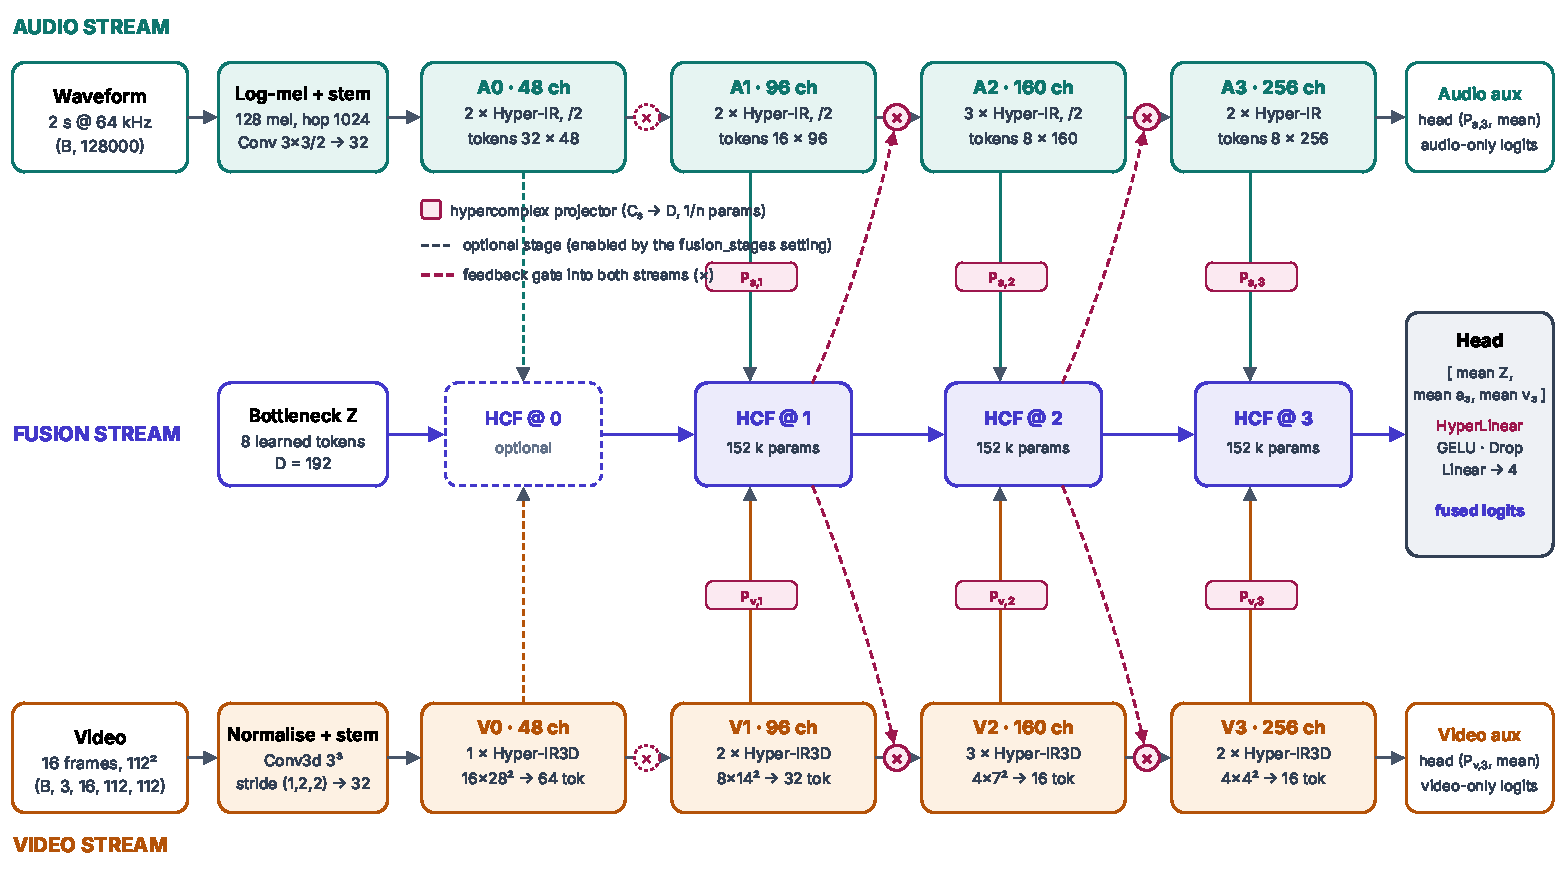
\includegraphics[width=\textwidth]{figures/arch_overview.pdf}
  \caption{HyperAVNet (default configuration: quaternion algebra, fusion stages $\mathcal{S}=\{1,2,3\}$,
  feedback enabled). Stage tokens of the audio and video backbones are projected by hypercomplex
  projectors $P_{a,s}$ and $P_{v,s}$ into a $D$-dimensional fusion space, where HCF blocks update the
  bottleneck tokens $\mathbf{Z}$. After each fused stage $s<S-1$, a zero-initialised gate ($\times$)
  modulates both streams. The classifier reads the pooled bottleneck and the pooled last-stage
  tokens; auxiliary heads supervise each modality on its own. Token shapes are for one 2\,s clip and
  $16\times112^{2}$ frames.}
  \label{fig:overview}
\end{figure*}

\subsection{Hypercomplex layers}
\label{sec:hyper}
Let $\mathbb{A}_n$ be a hypercomplex algebra of dimension $n\in\{2,4,8,16\}$ (complex numbers,
quaternions, octonions, sedenions, obtained by the Cayley--Dickson construction), with basis
$\{e_0,\dots,e_{n-1}\}$ and multiplication table
\begin{equation}
  e_i\,e_j = \sigma_{ij}\, e_{\pi(i,j)},
  \label{eq:table}
\end{equation}
with signs $\sigma_{ij}\in\{-1,+1\}$ and indices $\pi(i,j)\in\{0,\dots,n-1\}$.
A feature vector $\mathbf{x}\in\mathbb{R}^{d_{\mathrm{in}}}$ is split into $n$ components,
$\mathbf{x}=[\mathbf{x}_0;\dots;\mathbf{x}_{n-1}]$ with $\mathbf{x}_j\in\mathbb{R}^{d_{\mathrm{in}}/n}$,
i.e.\ it is read as $\sum_j \mathbf{x}_j e_j$. A hypercomplex weight
$\mathbf{W}=\sum_{k}\mathbf{W}_k e_k$ with real blocks $\mathbf{W}_k\in\mathbb{R}^{(d_{\mathrm{out}}/n)\times(d_{\mathrm{in}}/n)}$
acts on it by the algebra product, which in matrix form is
\begin{equation}
\begin{gathered}
  \mathbf{y}_i = \sum_{j=0}^{n-1} s_{ij}\,\mathbf{W}_{c(i,j)}\,\mathbf{x}_j + \mathbf{b}_i,\\
  \mathbf{K}(\mathbf{W}) = \big[\, s_{ij}\,\mathbf{W}_{c(i,j)} \,\big]_{i,j=0}^{n-1}\in\mathbb{R}^{d_{\mathrm{out}}\times d_{\mathrm{in}}},
\end{gathered}
  \label{eq:hlinear}
\end{equation}
where the block index $c(i,j)$ and sign $s_{ij}$ follow from Eq.~\eqref{eq:table}. For quaternions the
kernel takes the familiar Hamilton form (Fig.~\ref{fig:hamilton}),
\begin{equation}
  \mathbf{K} = \begin{bmatrix}
   \mathbf{W}_0 & \mathbf{W}_1 & \mathbf{W}_2 & \mathbf{W}_3\\
  -\mathbf{W}_1 & \mathbf{W}_0 & \mathbf{W}_3 & -\mathbf{W}_2\\
  -\mathbf{W}_2 & -\mathbf{W}_3 & \mathbf{W}_0 & \mathbf{W}_1\\
  -\mathbf{W}_3 & \mathbf{W}_2 & -\mathbf{W}_1 & \mathbf{W}_0
  \end{bmatrix}.
  \label{eq:hamilton}
\end{equation}
Every output component is thus a signed combination of \emph{every} input component through one
shared set of $n$ blocks, so the layer has
\begin{equation}
  |\theta_{\mathrm{hyper}}| = \tfrac{1}{n}\,d_{\mathrm{in}}d_{\mathrm{out}} + d_{\mathrm{out}}
  \;\;\text{vs.}\;\;
  |\theta_{\mathrm{real}}| = d_{\mathrm{in}}d_{\mathrm{out}} + d_{\mathrm{out}}
  \label{eq:params}
\end{equation}
parameters. A hypercomplex convolution applies the same block structure to the kernel tensor, with
$\mathbf{W}_k\in\mathbb{R}^{(C_{\mathrm{out}}/n)\times(C_{\mathrm{in}}/n)\times k_1\times\dots}$.
Weights are initialised in polar form: a modulus drawn from a $\chi$ distribution with $n$ degrees of
freedom (scaled by the Glorot variance), a uniform phase, and a unit-norm imaginary direction
\cite{bojesomo2024hypercomplex}. We write $\mathcal{H}_n(\cdot)$ for a hypercomplex linear or
convolutional layer. With $n=1$ it reduces to the real layer, which gives a matched real-valued
ablation with an identical code path.

\paragraph{Deployment.} Building $\mathbf{K}$ in Eq.~\eqref{eq:hlinear} at every forward pass
is only needed while training. After training, every $\mathcal{H}_n$ is \emph{reparameterised} into a
dense layer with weight $\mathbf{K}(\mathbf{W})$. The outputs are identical, and the run-time
overhead of kernel assembly disappears. The hypercomplex structure therefore reduces the number of
stored and optimised parameters (and the model's memory and transmission size) by up to $n\times$,
but \emph{not} the multiply--accumulate count, because $\mathbf{K}$ is dense.

\begin{figure}[t]
  \centering
  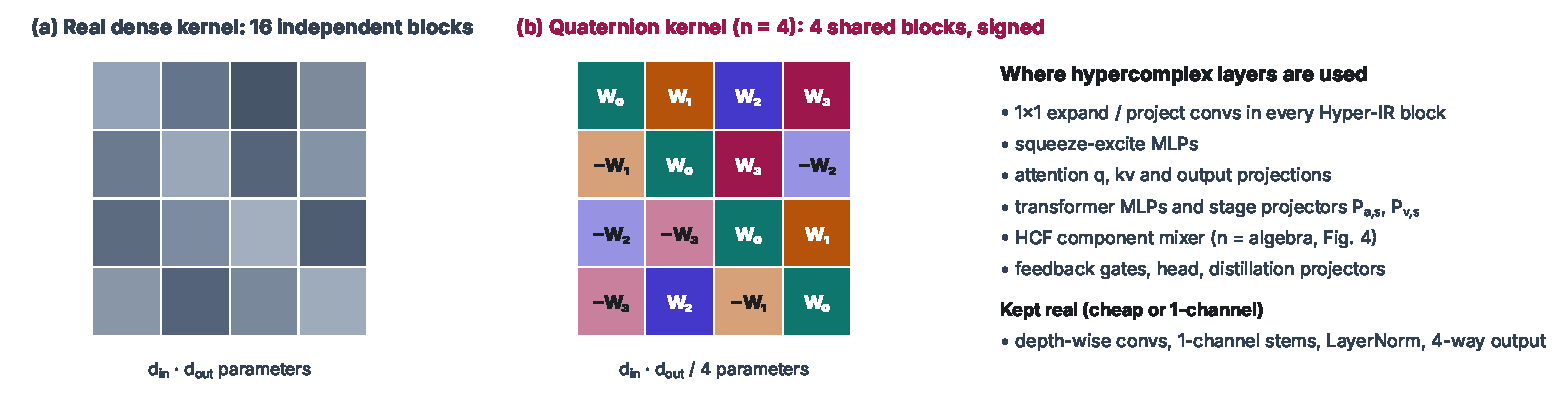
\includegraphics[width=\columnwidth]{figures/hamilton.pdf}
  \caption{Hamilton-product weight sharing. (a) A real kernel has $n^{2}$ independent blocks.
  (b) A quaternion kernel ($n=4$) re-uses four blocks with fixed signs (Eq.~\eqref{eq:hamilton}),
  which cuts the parameter count by $4\times$.}
  \label{fig:hamilton}
\end{figure}

\subsection{Hypercomplex backbones and stage tokens}
\label{sec:backbones}
\paragraph{Hyper-IR block.} Both backbones stack hypercomplex inverted-residual blocks
(Fig.~\ref{fig:hyperir}). For an input $\mathbf{h}\in\mathbb{R}^{C\times\Omega}$ ($\Omega$ is the 2-D
time--frequency grid for audio and the 3-D space--time grid for video) and expansion ratio $r=4$:
\begin{equation}
\begin{aligned}
  \mathbf{u} &= \operatorname{SiLU}\big(\operatorname{BN}(\mathcal{H}_n^{1\times1}(\mathbf{h}))\big)\in\mathbb{R}^{rC\times\Omega},\\
  \mathbf{v} &= \operatorname{SiLU}\big(\operatorname{BN}(\operatorname{DWConv}_{3}(\mathbf{u}))\big),\\
  \mathbf{w} &= \mathbf{v}\odot\sigma\big(\mathcal{H}_n(\operatorname{SiLU}(\mathcal{H}_n(\operatorname{GAP}(\mathbf{v}))))\big),\\
  \mathbf{h}' &= \mathbf{h} + \operatorname{DropPath}\big(\operatorname{BN}(\mathcal{H}_n^{1\times1}(\mathbf{w}))\big).
\end{aligned}
  \label{eq:hyperir}
\end{equation}
The two point-wise convolutions hold almost all of a block's parameters, so they are hypercomplex. The
depth-wise convolution stays real; it accounts for about 1\% of the parameters. The residual is used
when the shape is preserved.

\paragraph{Audio stream.} The waveform is converted to a log-mel spectrogram with the U-FFIA settings
(Hann window 2048, hop 1024, 128 mel bins at 64\,kHz, so a 2\,s clip gives $128\times126$),
normalised per mel bin by batch normalisation and augmented with SpecAugment during training. A
$3{\times}3$ stride-2 stem is followed by four Hyper-IR stages $s=0,\dots,3$ with widths
$(48,96,160,256)$ and depths $(2,2,3,2)$. A stage map $\mathbf{h}^{a}_{s}\in\mathbb{R}^{C_s\times T_s\times F_s}$
becomes time tokens by pooling over frequency:
\begin{equation}
  \mathbf{a}_s = \big[\operatorname{mean}_{F}(\mathbf{h}^{a}_s) + \operatorname{max}_{F}(\mathbf{h}^{a}_s)\big]^{\top}\in\mathbb{R}^{T_s\times C_s}.
  \label{eq:audiotokens}
\end{equation}
The max term keeps the short impulsive transients of feeding (chewing, tail slaps).

\paragraph{Video stream.} The frames are normalised and passed through a $3{\times}3{\times}3$ stem
(spatial stride 2) and four 3-D Hyper-IR stages of the same widths, with depths $(1,2,3,2)$ and
strides $(1,2,2)$, $(2,2,2)$, $(2,2,2)$, $(1,2,2)$. A stage map
$\mathbf{h}^{v}_{s}\in\mathbb{R}^{C_s\times T_s\times H_s\times W_s}$ is pooled to a $2\times2$ spatial grid
per time step, $\mathbf{v}_s\in\mathbb{R}^{4T_s\times C_s}$. This keeps coarse location (where the fish
aggregate) at a small token count.

\begin{figure}[t]
  \centering
  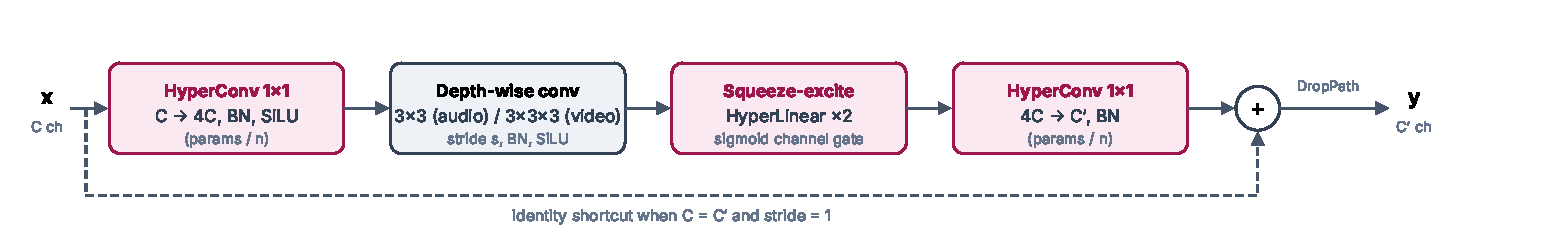
\includegraphics[width=\columnwidth]{figures/hyper_ir.pdf}
  \caption{Hypercomplex inverted-residual (Hyper-IR) block, Eq.~\eqref{eq:hyperir}. Hypercomplex
  layers are shaded; the depth-wise convolution is real.}
  \label{fig:hyperir}
\end{figure}

\paragraph{Pretrained backbones.} Any pretrained network can replace a student backbone if it exposes
four stages in the same token format. We use this for the teachers and for the teacher ablation
(Sec.~\ref{sec:setup}): PANNs CNN10/CNN14~\cite{kong2020panns}, EfficientAT~\cite{schmid2023efficientat},
AST~\cite{gong2021ast}, S3D~\cite{xie2018s3d}, X3D~\cite{feichtenhofer2020x3d},
MoViNet~\cite{kondratyuk2021movinets} and VideoMAE~\cite{tong2022videomae}. Their intermediate layers
supply the stage tokens.

\subsection{Hypercomplex component fusion}
\label{sec:hcf}
\paragraph{Projection.} Stage tokens are mapped into a shared $D$-dimensional space by hypercomplex
projectors with a learned modality embedding:
\begin{equation}
  \mathbf{A}_s = \operatorname{LN}\!\big(\mathcal{H}_n(\mathbf{a}_s)\big) + \mathbf{m}^{a},\qquad
  \mathbf{V}_s = \operatorname{LN}\!\big(\mathcal{H}_n(\mathbf{v}_s)\big) + \mathbf{m}^{v}.
  \label{eq:proj}
\end{equation}

\paragraph{Bottleneck state.} The fused representation lives in $N_b$ learned bottleneck tokens
$\mathbf{Z}\in\mathbb{R}^{N_b\times D}$ (we use $N_b=8$, $D=192$), shared across stages.

\paragraph{HCF block.} At a fusion stage $s$, the bottleneck first reads each modality with its own
hypercomplex cross-attention:
\begin{equation}
\begin{aligned}
  \mathbf{Z}^{a} &= \mathbf{Z} + \operatorname{XAttn}_{n}\big(\operatorname{LN}\mathbf{Z},\,\operatorname{LN}\mathbf{A}_s\big),\\
  \mathbf{Z}^{v} &= \mathbf{Z} + \operatorname{XAttn}_{n}\big(\operatorname{LN}\mathbf{Z},\,\operatorname{LN}\mathbf{V}_s\big),
\end{aligned}
  \label{eq:xattn}
\end{equation}
where $\operatorname{XAttn}_n$ is multi-head attention whose query, key, value and output projections
are hypercomplex (shown for one head of width $d_h$):
\begin{equation*}
  \operatorname{XAttn}_n(\mathbf{Q},\mathbf{C})=\mathcal{H}_n\Big(\operatorname{softmax}\Big(\tfrac{\mathcal{H}_n(\mathbf{Q})\,\mathcal{H}_n(\mathbf{C})^{\top}}{\sqrt{d_h}}\Big)\mathcal{H}_n(\mathbf{C})\Big).
\end{equation*} The shared
state, the two modality views and their interaction then form the components of one element of
$\mathbb{A}_m$:
\begin{equation}
  \mathbf{q} = \mathbf{Z}\,e_0 + \mathbf{Z}^{a}\,e_1 + \mathbf{Z}^{v}\,e_2 + \big(\hat{\mathbf{Z}}^{a}\odot\hat{\mathbf{Z}}^{v}\big)\,e_3,
  \label{eq:components}
\end{equation}
for $m=4$,
with $\hat{\cdot}=\operatorname{LN}(\cdot)$. The octonion variant ($m=8$) appends
$(\mathbf{Z}^{a}-\mathbf{Z}^{v})e_4$, $(\hat{\mathbf{Z}}\odot\hat{\mathbf{Z}}^{a})e_5$,
$(\hat{\mathbf{Z}}\odot\hat{\mathbf{Z}}^{v})e_6$ and
$(\hat{\mathbf{Z}}\odot\hat{\mathbf{Z}}^{a}\odot\hat{\mathbf{Z}}^{v})e_7$; the complex variant ($m=2$) uses
$(\mathbf{Z}^{a},\mathbf{Z}^{v})$. The components are mixed by a single Hamilton product, followed by a
hypercomplex MLP:
\begin{equation}
\begin{aligned}
  \mathbf{Z} &\leftarrow \mathbf{Z} + \boldsymbol{\gamma}_1\odot \mathcal{H}_m(\mathbf{q}),\\
  \mathbf{Z} &\leftarrow \mathbf{Z} + \boldsymbol{\gamma}_2\odot \operatorname{MLP}_n(\operatorname{LN}\mathbf{Z}),
\end{aligned}
  \label{eq:mix}
\end{equation}
where $\mathcal{H}_m:\mathbb{R}^{mD}\to\mathbb{R}^{D}$ is a hypercomplex linear layer of algebra
$\mathbb{A}_m$ and $\boldsymbol{\gamma}_{1,2}$ are LayerScale vectors~\cite{touvron2021cait}, initialised to
$10^{-2}$. By Eq.~\eqref{eq:hlinear}, each output component of $\mathcal{H}_m$ is a signed mixture of
the shared state, both modality views and their multiplicative agreement, all through one set of
$m$ blocks. The mixer has $D^{2}$ parameters \emph{for every} $m$, against $mD^{2}$ for a dense mixer, so
the octonion variant adds four interaction terms at no parameter cost. Unlike attention bottlenecks
that attend to the modalities one after the other~\cite{nagrani2021mbt}, HCF reads both modalities
in parallel and combines them in one algebraic product (Fig.~\ref{fig:hcf}).

\begin{figure*}[t]
  \centering
  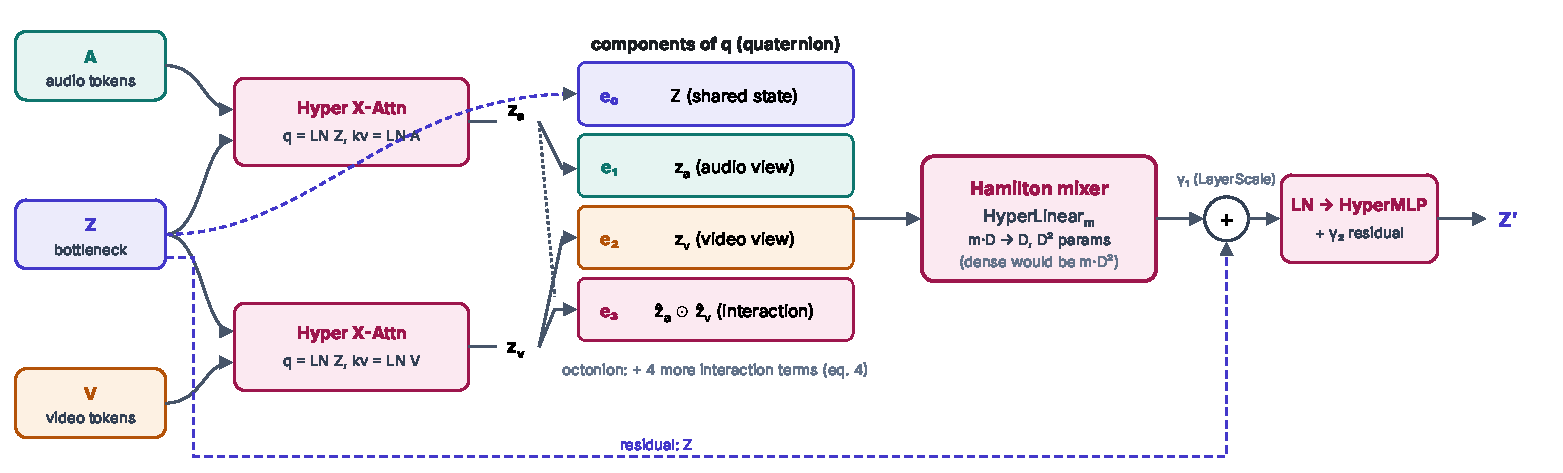
\includegraphics[width=0.9\textwidth]{figures/hcf_block.pdf}
  \caption{Hypercomplex component fusion (HCF), Eqs.~\eqref{eq:xattn}--\eqref{eq:mix}. The modality
  views and their interaction are the components of one quaternion and are mixed by a single
  Hamilton product.}
  \label{fig:hcf}
\end{figure*}

\subsection{Deep-to-early fusion schedule with cross-modal feedback}
\label{sec:schedule}
The set $\mathcal{S}\subseteq\{0,\dots,S-1\}$ selects the stages at which an HCF block is attached:
\begin{equation}
  \mathbf{Z}^{(s+1)} = \begin{cases}\operatorname{HCF}_s\big(\mathbf{Z}^{(s)},\mathbf{A}_s,\mathbf{V}_s\big), & s\in\mathcal{S},\\ \mathbf{Z}^{(s)}, & \text{otherwise,}\end{cases}
  \label{eq:schedule}
\end{equation}
with $\mathbf{Z}^{(0)}=\mathbf{Z}_{\mathrm{init}}$ the learned bottleneck tokens.
Varying $\mathcal{S}$ from $\{S-1\}$ (late fusion) through $\{S-2,S-1\}$ and so on to $\{0,\dots,S-1\}$
gives a controlled \emph{deep-to-early} study of where audio--visual fusion helps. Because the student
backbones are executed stage by stage, the fused state is also fed back into both streams after each
fused stage $s<S-1$:
\begin{equation}
  \mathbf{h}^{m}_s \leftarrow \mathbf{h}^{m}_s\odot\big(1+\tanh(\mathcal{G}^{m}_s\,\bar{\mathbf{z}}^{(s+1)})\big),\quad m\in\{a,v\},
  \label{eq:feedback}
\end{equation}
where $\bar{\mathbf{z}}=\operatorname{mean}_{N_b}(\mathbf{Z})$, the gates
$\mathcal{G}^{m}_s$ are hypercomplex linear maps $\mathbb{R}^{D}\to\mathbb{R}^{C_s}$, and the
product broadcasts over $\Omega$. The gates are \emph{initialised to zero}, so training starts exactly
at the feedback-free model. The network then learns how strongly each modality should condition the
other's later features. This is genuine early fusion, as opposed to fusing independently computed
features.

\subsection{Prediction heads and modality dropout}
\label{sec:heads}
With $\bar{\mathbf{z}}=\operatorname{mean}(\operatorname{LN}\mathbf{Z}^{(S)})$,
$\bar{\mathbf{a}}=\operatorname{mean}(\operatorname{LN}\mathbf{A}_{S-1})$ and
$\bar{\mathbf{v}}=\operatorname{mean}(\operatorname{LN}\mathbf{V}_{S-1})$, the fused and auxiliary logits are
\begin{equation}
\begin{gathered}
  \boldsymbol{\ell} = \mathbf{W}_o\,\operatorname{GELU}\big(\mathcal{H}_n[\bar{\mathbf{z}};\,\mu_a\bar{\mathbf{a}};\,\mu_v\bar{\mathbf{v}}]\big),\\
  \boldsymbol{\ell}^{a} = \mathbf{W}_a\bar{\mathbf{a}},\qquad \boldsymbol{\ell}^{v} = \mathbf{W}_v\bar{\mathbf{v}}.
\end{gathered}
  \label{eq:heads}
\end{equation}
Here $\mu_a,\mu_v\in\{0,1\}$ are per-sample modality masks. During training,
$(\mu_a,\mu_v)=(0,1)$ with probability $p$, $(1,0)$ with probability $p$, and $(1,1)$ otherwise. In the
notation of~\cite{cui2024uffia}, $p_{av}=1-2p$ and $p_a=p_v=p$. The same mask multiplies every fusion
input $\mathbf{A}_s,\mathbf{V}_s$, so a dropped modality is absent everywhere. The auxiliary heads always see
their own modality, which keeps both branches trained regardless of $p$. At test time, forcing
$\mu_a=0$ or $\mu_v=0$ evaluates the model with a missing modality.

\subsection{Training objective and multi-level distillation}
\label{sec:objective}
The supervised loss combines label-smoothed cross-entropy on the fused logits with the two
auxiliary terms:
\begin{equation}
  \mathcal{L}_{\mathrm{sup}} = \operatorname{CE}_{\epsilon}(\boldsymbol{\ell},y)
   + \tfrac{\lambda_{\mathrm{aux}}}{2}\!\!\sum_{m\in\{a,v\}}\!\!\operatorname{CE}_{\epsilon}(\boldsymbol{\ell}^{m},y).
  \label{eq:sup}
\end{equation}
A frozen teacher $g$ with the same output structure (pretrained backbones and HCF fusion) provides
three further signals. At the \emph{logit level}, with temperature $\tau$:
\begin{equation}
  \mathcal{L}_{\mathrm{KD}} = \tau^{2}\,\mathrm{KL}\big(\boldsymbol{\ell}^{g}\,\|\,\boldsymbol{\ell}\big)_{\tau}
   + \tfrac{\lambda_{u}\tau^{2}}{2}\!\!\sum_{m\in\{a,v\}}\!\!\mathrm{KL}\big(\boldsymbol{\ell}^{g,m}\,\|\,\boldsymbol{\ell}^{m}\big)_{\tau},
  \label{eq:kd}
\end{equation}
with $\mathrm{KL}(\mathbf{u}\,\|\,\mathbf{w})_{\tau}=\mathrm{KL}\big(\operatorname{softmax}(\mathbf{u}/\tau)\,\|\,\operatorname{softmax}(\mathbf{w}/\tau)\big)$,
which distils each unimodal head from its counterpart in the teacher. U-FFIA's variant~\cite{cui2024uffia}
softens only the teacher, $\mathrm{KL}(\operatorname{softmax}(\boldsymbol{\ell}^{g}/\tau)\,\|\,\operatorname{softmax}(\boldsymbol{\ell}))$,
and is evaluated as an ablation. At the \emph{embedding level}, small hypercomplex projectors
$\mathcal{P}_k$ align the student's pooled embeddings with the teacher's:
\begin{equation}
  \mathcal{L}_{\mathrm{feat}} = \tfrac{1}{3}\!\!\sum_{k\in\{\bar{\mathbf{z}},\bar{\mathbf{a}},\bar{\mathbf{v}}\}}\!\!
  \big(1-\cos(\mathcal{P}_k(k),\,k^{g})\big).
  \label{eq:feat}
\end{equation}
At the \emph{relation level}~\cite{park2019rkd}, the within-batch similarity structure of the fused
embeddings is matched:
\begin{equation}
  \mathcal{L}_{\mathrm{rel}} = \operatorname{SmoothL1}\big(\mathbf{R}(\bar{\mathbf{z}}_{1:B}),\,\mathbf{R}(\bar{\mathbf{z}}^{g}_{1:B})\big),
  \label{eq:rel}
\end{equation}
where $\mathbf{R}(\mathbf{U})_{ij}=\mathbf{u}_i^{\top}\mathbf{u}_j/(\|\mathbf{u}_i\|\|\mathbf{u}_j\|)$ is the cosine-similarity matrix of a batch of size $B$.
The full objective is
\begin{equation}
  \mathcal{L} = \mathcal{L}_{\mathrm{sup}} + \alpha\,\mathcal{L}_{\mathrm{KD}} + \beta\,\mathcal{L}_{\mathrm{feat}} + \gamma\,\mathcal{L}_{\mathrm{rel}},
  \label{eq:total}
\end{equation}
with $\epsilon=0.1$, $\lambda_{\mathrm{aux}}=0.3$, $\lambda_u=0.5$, $\tau=2$, $\alpha=0.7$, $\beta=1$ and $\gamma=0.5$.
Training proceeds in two stages: the teacher is trained with $\mathcal{L}_{\mathrm{sup}}$ and frozen, then
the student is trained with Eq.~\eqref{eq:total}.

\begin{figure*}[t]
  \centering
  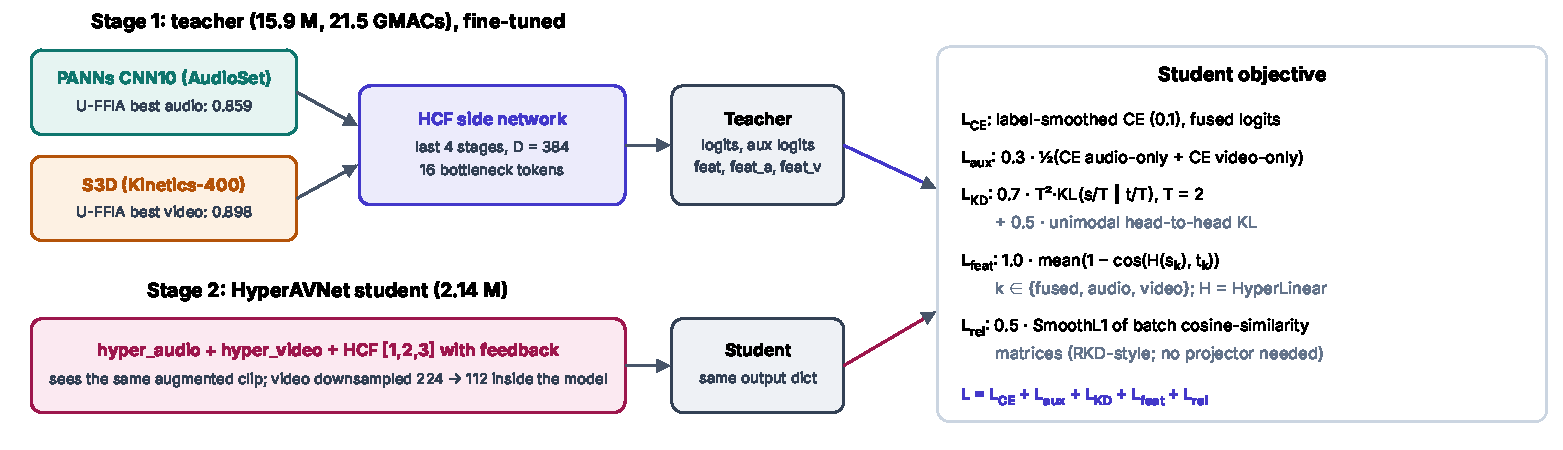
\includegraphics[width=0.92\textwidth]{figures/distillation.pdf}
  \caption{Two-stage training. A teacher built from pretrained audio and video backbones and HCF fusion
  is trained first and frozen. The HyperAVNet student is then trained with the supervised loss plus
  logit-, embedding- and relation-level distillation (Eq.~\eqref{eq:total}).}
  \label{fig:distill}
\end{figure*}

\subsection{Complexity}
\label{sec:complexity}
By Eq.~\eqref{eq:params}, every hypercomplex projection stores $1/n$ of the real parameters. Only the
stems, the depth-wise convolutions, normalisation layers and the final $4$-way classifier stay real.
For the default student ($n=4$), the network has 2.14\,M parameters against 7.88\,M for the identical
real network ($n=1$), and 1.24\,M (octonion) or 0.78\,M (sedenion) for higher algebras. Compute is
1.18\,GMACs per clip for every $n$ (16 frames at $112^{2}$ and 2\,s of audio). The added cost of a
fusion stage is about 0.17\,M parameters and under 0.02\,GMACs.
 in any paper.
%  Requires: amsmath, amssymb, bm, booktabs, graphicx, (cleveref optional).
% ============================================================================
\section{Methodology}
\label{sec:method}

\subsection{Problem formulation}
\label{sec:problem}
Each sample of AV-FFIA is a synchronised two-second clip $(\mathbf{x}^{a}, \mathbf{X}^{v})$, where
$\mathbf{x}^{a}\in\mathbb{R}^{L}$ is the hydrophone waveform ($L = 2f_s$, $f_s = 64$\,kHz) and
$\mathbf{X}^{v}\in[0,1]^{3\times T\times H\times W}$ holds $T$ RGB frames sampled uniformly from the
overhead camera. The label $y\in\mathcal{Y}=\{\textsc{None},\textsc{Weak},\textsc{Medium},\textsc{Strong}\}$
is the feeding intensity. We learn $f_{\theta}:(\mathbf{x}^{a},\mathbf{X}^{v})\mapsto\mathbf{p}\in\Delta^{|\mathcal{Y}|-1}$ with
two goals that pull in opposite directions: high accuracy, robust to the acoustic and visual
corruptions typical of aquaculture (bubbles, pumps, low light, reflections), and a small
parameter and compute budget for on-site deployment.

HyperAVNet (Fig.~\ref{fig:overview}) has four parts. Two hypercomplex backbones map each modality to a
hierarchy of \emph{stage tokens} (Sec.~\ref{sec:backbones}). A set of shared \emph{bottleneck tokens}
is updated by hypercomplex component fusion (HCF) blocks attached at a configurable subset of
stages, with zero-initialised cross-modal feedback into both streams (Secs.~\ref{sec:hcf},~\ref{sec:schedule}).
Fused and unimodal heads produce the predictions (Sec.~\ref{sec:heads}). The model is trained with a
multi-level distillation objective from a pretrained audio-visual teacher (Sec.~\ref{sec:objective}).

\begin{figure*}[t]
  \centering
  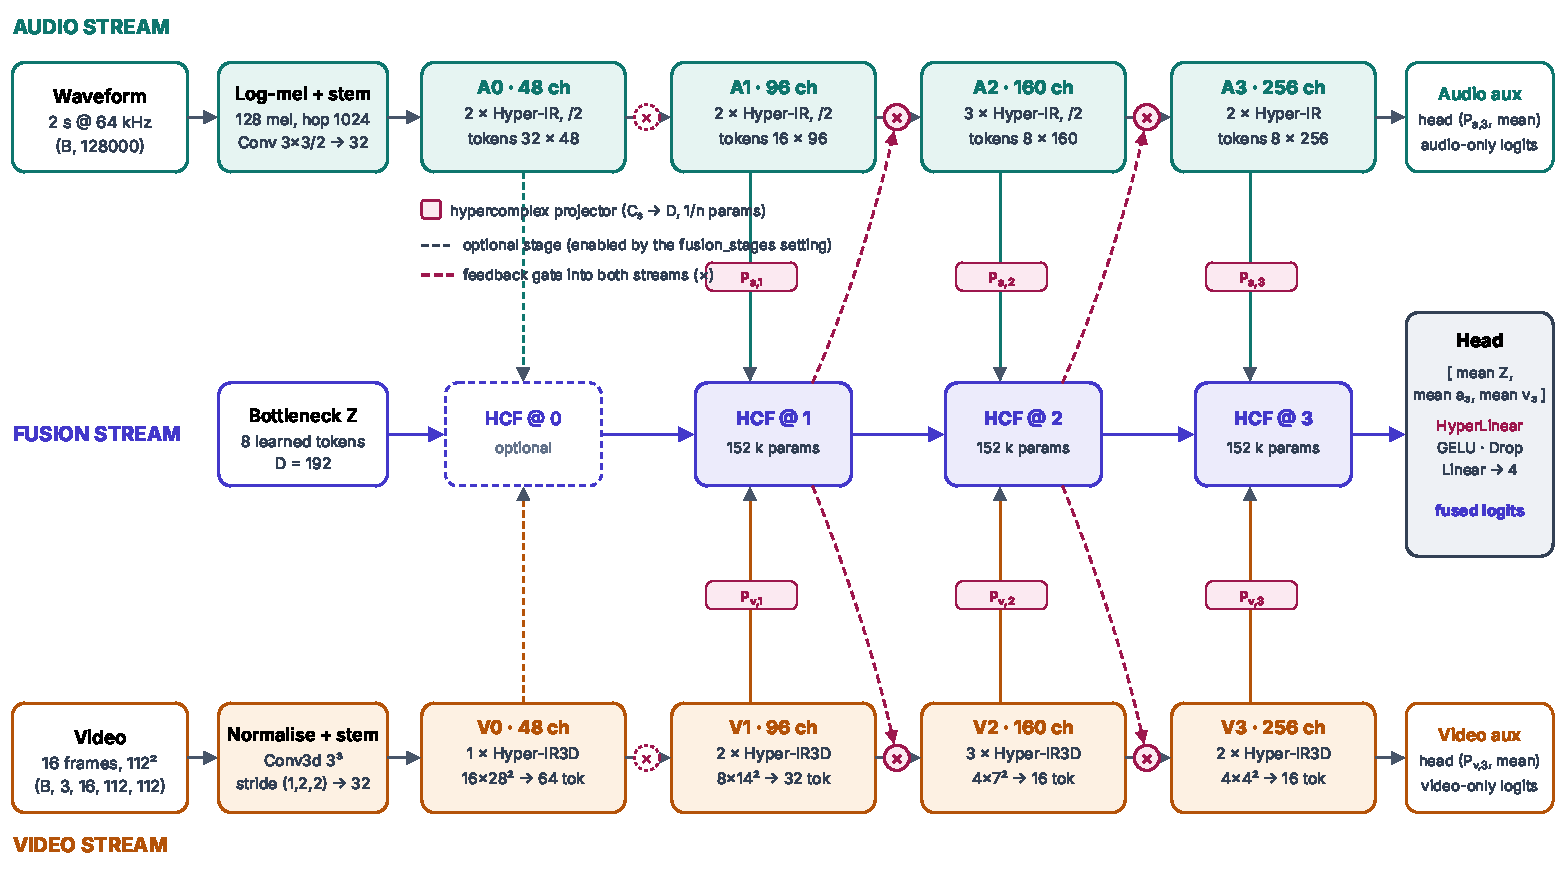
\includegraphics[width=\textwidth]{figures/arch_overview.pdf}
  \caption{HyperAVNet (default configuration: quaternion algebra, fusion stages $\mathcal{S}=\{1,2,3\}$,
  feedback enabled). Stage tokens of the audio and video backbones are projected by hypercomplex
  projectors $P_{a,s}$ and $P_{v,s}$ into a $D$-dimensional fusion space, where HCF blocks update the
  bottleneck tokens $\mathbf{Z}$. After each fused stage $s<S-1$, a zero-initialised gate ($\times$)
  modulates both streams. The classifier reads the pooled bottleneck and the pooled last-stage
  tokens; auxiliary heads supervise each modality on its own. Token shapes are for one 2\,s clip and
  $16\times112^{2}$ frames.}
  \label{fig:overview}
\end{figure*}

\subsection{Hypercomplex layers}
\label{sec:hyper}
Let $\mathbb{A}_n$ be a hypercomplex algebra of dimension $n\in\{2,4,8,16\}$ (complex numbers,
quaternions, octonions, sedenions, obtained by the Cayley--Dickson construction), with basis
$\{e_0,\dots,e_{n-1}\}$ and multiplication table
\begin{equation}
  e_i\,e_j = \sigma_{ij}\, e_{\pi(i,j)},
  \label{eq:table}
\end{equation}
with signs $\sigma_{ij}\in\{-1,+1\}$ and indices $\pi(i,j)\in\{0,\dots,n-1\}$.
A feature vector $\mathbf{x}\in\mathbb{R}^{d_{\mathrm{in}}}$ is split into $n$ components,
$\mathbf{x}=[\mathbf{x}_0;\dots;\mathbf{x}_{n-1}]$ with $\mathbf{x}_j\in\mathbb{R}^{d_{\mathrm{in}}/n}$,
i.e.\ it is read as $\sum_j \mathbf{x}_j e_j$. A hypercomplex weight
$\mathbf{W}=\sum_{k}\mathbf{W}_k e_k$ with real blocks $\mathbf{W}_k\in\mathbb{R}^{(d_{\mathrm{out}}/n)\times(d_{\mathrm{in}}/n)}$
acts on it by the algebra product, which in matrix form is
\begin{equation}
\begin{gathered}
  \mathbf{y}_i = \sum_{j=0}^{n-1} s_{ij}\,\mathbf{W}_{c(i,j)}\,\mathbf{x}_j + \mathbf{b}_i,\\
  \mathbf{K}(\mathbf{W}) = \big[\, s_{ij}\,\mathbf{W}_{c(i,j)} \,\big]_{i,j=0}^{n-1}\in\mathbb{R}^{d_{\mathrm{out}}\times d_{\mathrm{in}}},
\end{gathered}
  \label{eq:hlinear}
\end{equation}
where the block index $c(i,j)$ and sign $s_{ij}$ follow from Eq.~\eqref{eq:table}. For quaternions the
kernel takes the familiar Hamilton form (Fig.~\ref{fig:hamilton}),
\begin{equation}
  \mathbf{K} = \begin{bmatrix}
   \mathbf{W}_0 & \mathbf{W}_1 & \mathbf{W}_2 & \mathbf{W}_3\\
  -\mathbf{W}_1 & \mathbf{W}_0 & \mathbf{W}_3 & -\mathbf{W}_2\\
  -\mathbf{W}_2 & -\mathbf{W}_3 & \mathbf{W}_0 & \mathbf{W}_1\\
  -\mathbf{W}_3 & \mathbf{W}_2 & -\mathbf{W}_1 & \mathbf{W}_0
  \end{bmatrix}.
  \label{eq:hamilton}
\end{equation}
Every output component is thus a signed combination of \emph{every} input component through one
shared set of $n$ blocks, so the layer has
\begin{equation}
  |\theta_{\mathrm{hyper}}| = \tfrac{1}{n}\,d_{\mathrm{in}}d_{\mathrm{out}} + d_{\mathrm{out}}
  \;\;\text{vs.}\;\;
  |\theta_{\mathrm{real}}| = d_{\mathrm{in}}d_{\mathrm{out}} + d_{\mathrm{out}}
  \label{eq:params}
\end{equation}
parameters. A hypercomplex convolution applies the same block structure to the kernel tensor, with
$\mathbf{W}_k\in\mathbb{R}^{(C_{\mathrm{out}}/n)\times(C_{\mathrm{in}}/n)\times k_1\times\dots}$.
Weights are initialised in polar form: a modulus drawn from a $\chi$ distribution with $n$ degrees of
freedom (scaled by the Glorot variance), a uniform phase, and a unit-norm imaginary direction
\cite{bojesomo2024hypercomplex}. We write $\mathcal{H}_n(\cdot)$ for a hypercomplex linear or
convolutional layer. With $n=1$ it reduces to the real layer, which gives a matched real-valued
ablation with an identical code path.

\paragraph{Deployment.} Building $\mathbf{K}$ in Eq.~\eqref{eq:hlinear} at every forward pass
is only needed while training. After training, every $\mathcal{H}_n$ is \emph{reparameterised} into a
dense layer with weight $\mathbf{K}(\mathbf{W})$. The outputs are identical, and the run-time
overhead of kernel assembly disappears. The hypercomplex structure therefore reduces the number of
stored and optimised parameters (and the model's memory and transmission size) by up to $n\times$,
but \emph{not} the multiply--accumulate count, because $\mathbf{K}$ is dense.

\begin{figure}[t]
  \centering
  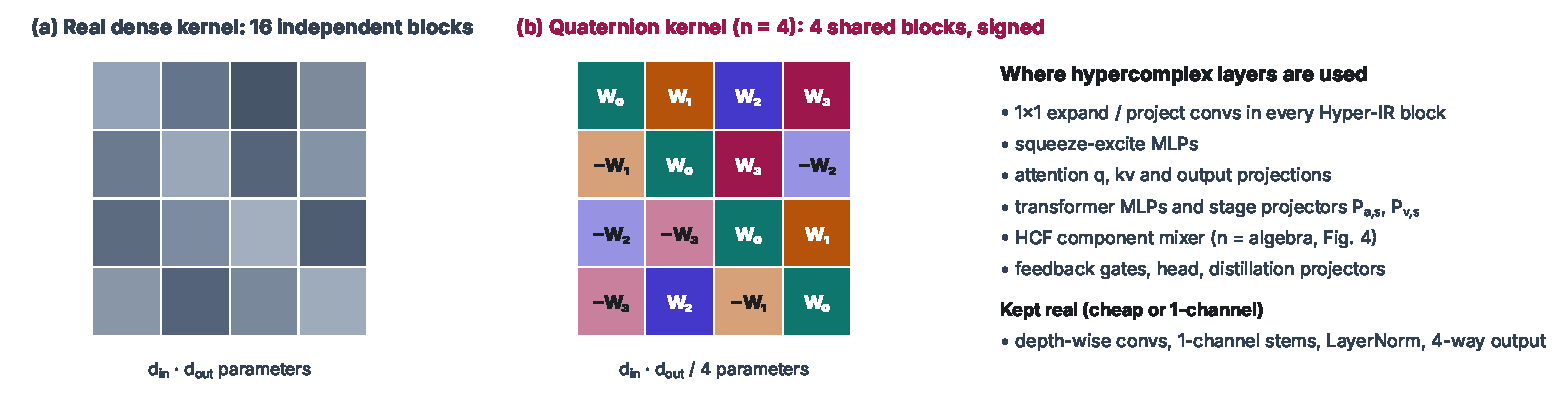
\includegraphics[width=\columnwidth]{figures/hamilton.pdf}
  \caption{Hamilton-product weight sharing. (a) A real kernel has $n^{2}$ independent blocks.
  (b) A quaternion kernel ($n=4$) re-uses four blocks with fixed signs (Eq.~\eqref{eq:hamilton}),
  which cuts the parameter count by $4\times$.}
  \label{fig:hamilton}
\end{figure}

\subsection{Hypercomplex backbones and stage tokens}
\label{sec:backbones}
\paragraph{Hyper-IR block.} Both backbones stack hypercomplex inverted-residual blocks
(Fig.~\ref{fig:hyperir}). For an input $\mathbf{h}\in\mathbb{R}^{C\times\Omega}$ ($\Omega$ is the 2-D
time--frequency grid for audio and the 3-D space--time grid for video) and expansion ratio $r=4$:
\begin{equation}
\begin{aligned}
  \mathbf{u} &= \operatorname{SiLU}\big(\operatorname{BN}(\mathcal{H}_n^{1\times1}(\mathbf{h}))\big)\in\mathbb{R}^{rC\times\Omega},\\
  \mathbf{v} &= \operatorname{SiLU}\big(\operatorname{BN}(\operatorname{DWConv}_{3}(\mathbf{u}))\big),\\
  \mathbf{w} &= \mathbf{v}\odot\sigma\big(\mathcal{H}_n(\operatorname{SiLU}(\mathcal{H}_n(\operatorname{GAP}(\mathbf{v}))))\big),\\
  \mathbf{h}' &= \mathbf{h} + \operatorname{DropPath}\big(\operatorname{BN}(\mathcal{H}_n^{1\times1}(\mathbf{w}))\big).
\end{aligned}
  \label{eq:hyperir}
\end{equation}
The two point-wise convolutions hold almost all of a block's parameters, so they are hypercomplex. The
depth-wise convolution stays real; it accounts for about 1\% of the parameters. The residual is used
when the shape is preserved.

\paragraph{Audio stream.} The waveform is converted to a log-mel spectrogram with the U-FFIA settings
(Hann window 2048, hop 1024, 128 mel bins at 64\,kHz, so a 2\,s clip gives $128\times126$),
normalised per mel bin by batch normalisation and augmented with SpecAugment during training. A
$3{\times}3$ stride-2 stem is followed by four Hyper-IR stages $s=0,\dots,3$ with widths
$(48,96,160,256)$ and depths $(2,2,3,2)$. A stage map $\mathbf{h}^{a}_{s}\in\mathbb{R}^{C_s\times T_s\times F_s}$
becomes time tokens by pooling over frequency:
\begin{equation}
  \mathbf{a}_s = \big[\operatorname{mean}_{F}(\mathbf{h}^{a}_s) + \operatorname{max}_{F}(\mathbf{h}^{a}_s)\big]^{\top}\in\mathbb{R}^{T_s\times C_s}.
  \label{eq:audiotokens}
\end{equation}
The max term keeps the short impulsive transients of feeding (chewing, tail slaps).

\paragraph{Video stream.} The frames are normalised and passed through a $3{\times}3{\times}3$ stem
(spatial stride 2) and four 3-D Hyper-IR stages of the same widths, with depths $(1,2,3,2)$ and
strides $(1,2,2)$, $(2,2,2)$, $(2,2,2)$, $(1,2,2)$. A stage map
$\mathbf{h}^{v}_{s}\in\mathbb{R}^{C_s\times T_s\times H_s\times W_s}$ is pooled to a $2\times2$ spatial grid
per time step, $\mathbf{v}_s\in\mathbb{R}^{4T_s\times C_s}$. This keeps coarse location (where the fish
aggregate) at a small token count.

\begin{figure}[t]
  \centering
  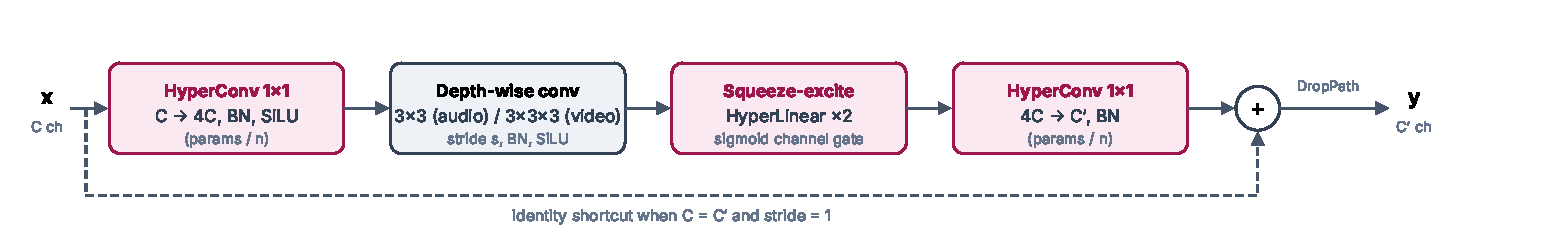
\includegraphics[width=\columnwidth]{figures/hyper_ir.pdf}
  \caption{Hypercomplex inverted-residual (Hyper-IR) block, Eq.~\eqref{eq:hyperir}. Hypercomplex
  layers are shaded; the depth-wise convolution is real.}
  \label{fig:hyperir}
\end{figure}

\paragraph{Pretrained backbones.} Any pretrained network can replace a student backbone if it exposes
four stages in the same token format. We use this for the teachers and for the teacher ablation
(Sec.~\ref{sec:setup}): PANNs CNN10/CNN14~\cite{kong2020panns}, EfficientAT~\cite{schmid2023efficientat},
AST~\cite{gong2021ast}, S3D~\cite{xie2018s3d}, X3D~\cite{feichtenhofer2020x3d},
MoViNet~\cite{kondratyuk2021movinets} and VideoMAE~\cite{tong2022videomae}. Their intermediate layers
supply the stage tokens.

\subsection{Hypercomplex component fusion}
\label{sec:hcf}
\paragraph{Projection.} Stage tokens are mapped into a shared $D$-dimensional space by hypercomplex
projectors with a learned modality embedding:
\begin{equation}
  \mathbf{A}_s = \operatorname{LN}\!\big(\mathcal{H}_n(\mathbf{a}_s)\big) + \mathbf{m}^{a},\qquad
  \mathbf{V}_s = \operatorname{LN}\!\big(\mathcal{H}_n(\mathbf{v}_s)\big) + \mathbf{m}^{v}.
  \label{eq:proj}
\end{equation}

\paragraph{Bottleneck state.} The fused representation lives in $N_b$ learned bottleneck tokens
$\mathbf{Z}\in\mathbb{R}^{N_b\times D}$ (we use $N_b=8$, $D=192$), shared across stages.

\paragraph{HCF block.} At a fusion stage $s$, the bottleneck first reads each modality with its own
hypercomplex cross-attention:
\begin{equation}
\begin{aligned}
  \mathbf{Z}^{a} &= \mathbf{Z} + \operatorname{XAttn}_{n}\big(\operatorname{LN}\mathbf{Z},\,\operatorname{LN}\mathbf{A}_s\big),\\
  \mathbf{Z}^{v} &= \mathbf{Z} + \operatorname{XAttn}_{n}\big(\operatorname{LN}\mathbf{Z},\,\operatorname{LN}\mathbf{V}_s\big),
\end{aligned}
  \label{eq:xattn}
\end{equation}
where $\operatorname{XAttn}_n$ is multi-head attention whose query, key, value and output projections
are hypercomplex (shown for one head of width $d_h$):
\begin{equation*}
  \operatorname{XAttn}_n(\mathbf{Q},\mathbf{C})=\mathcal{H}_n\Big(\operatorname{softmax}\Big(\tfrac{\mathcal{H}_n(\mathbf{Q})\,\mathcal{H}_n(\mathbf{C})^{\top}}{\sqrt{d_h}}\Big)\mathcal{H}_n(\mathbf{C})\Big).
\end{equation*} The shared
state, the two modality views and their interaction then form the components of one element of
$\mathbb{A}_m$:
\begin{equation}
  \mathbf{q} = \mathbf{Z}\,e_0 + \mathbf{Z}^{a}\,e_1 + \mathbf{Z}^{v}\,e_2 + \big(\hat{\mathbf{Z}}^{a}\odot\hat{\mathbf{Z}}^{v}\big)\,e_3,
  \label{eq:components}
\end{equation}
for $m=4$,
with $\hat{\cdot}=\operatorname{LN}(\cdot)$. The octonion variant ($m=8$) appends
$(\mathbf{Z}^{a}-\mathbf{Z}^{v})e_4$, $(\hat{\mathbf{Z}}\odot\hat{\mathbf{Z}}^{a})e_5$,
$(\hat{\mathbf{Z}}\odot\hat{\mathbf{Z}}^{v})e_6$ and
$(\hat{\mathbf{Z}}\odot\hat{\mathbf{Z}}^{a}\odot\hat{\mathbf{Z}}^{v})e_7$; the complex variant ($m=2$) uses
$(\mathbf{Z}^{a},\mathbf{Z}^{v})$. The components are mixed by a single Hamilton product, followed by a
hypercomplex MLP:
\begin{equation}
\begin{aligned}
  \mathbf{Z} &\leftarrow \mathbf{Z} + \boldsymbol{\gamma}_1\odot \mathcal{H}_m(\mathbf{q}),\\
  \mathbf{Z} &\leftarrow \mathbf{Z} + \boldsymbol{\gamma}_2\odot \operatorname{MLP}_n(\operatorname{LN}\mathbf{Z}),
\end{aligned}
  \label{eq:mix}
\end{equation}
where $\mathcal{H}_m:\mathbb{R}^{mD}\to\mathbb{R}^{D}$ is a hypercomplex linear layer of algebra
$\mathbb{A}_m$ and $\boldsymbol{\gamma}_{1,2}$ are LayerScale vectors~\cite{touvron2021cait}, initialised to
$10^{-2}$. By Eq.~\eqref{eq:hlinear}, each output component of $\mathcal{H}_m$ is a signed mixture of
the shared state, both modality views and their multiplicative agreement, all through one set of
$m$ blocks. The mixer has $D^{2}$ parameters \emph{for every} $m$, against $mD^{2}$ for a dense mixer, so
the octonion variant adds four interaction terms at no parameter cost. Unlike attention bottlenecks
that attend to the modalities one after the other~\cite{nagrani2021mbt}, HCF reads both modalities
in parallel and combines them in one algebraic product (Fig.~\ref{fig:hcf}).

\begin{figure*}[t]
  \centering
  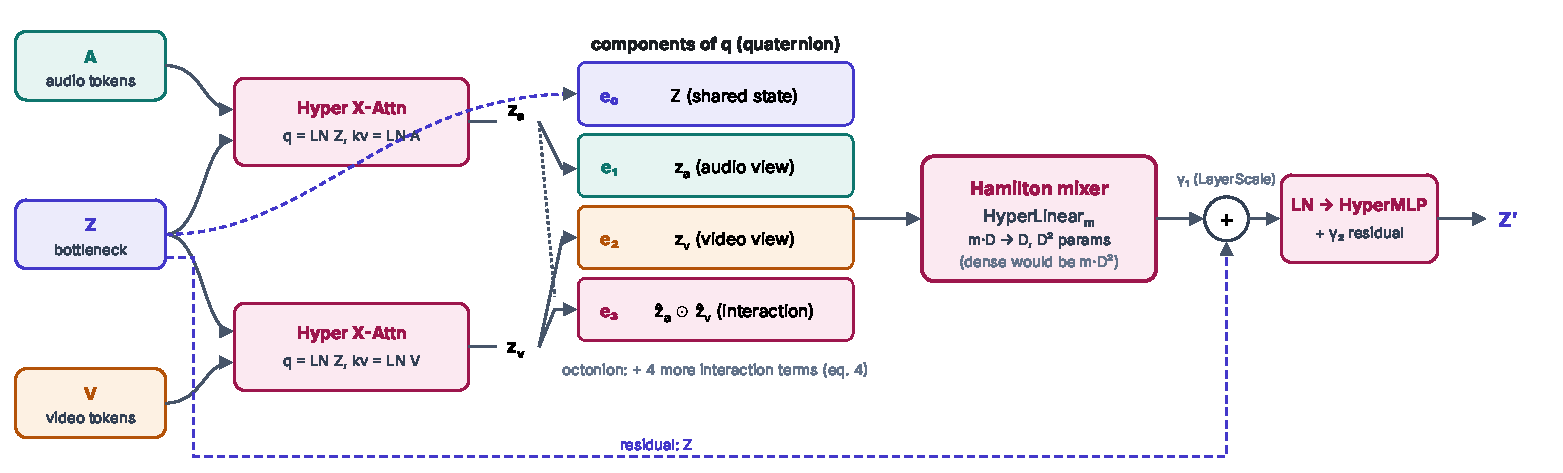
\includegraphics[width=0.9\textwidth]{figures/hcf_block.pdf}
  \caption{Hypercomplex component fusion (HCF), Eqs.~\eqref{eq:xattn}--\eqref{eq:mix}. The modality
  views and their interaction are the components of one quaternion and are mixed by a single
  Hamilton product.}
  \label{fig:hcf}
\end{figure*}

\subsection{Deep-to-early fusion schedule with cross-modal feedback}
\label{sec:schedule}
The set $\mathcal{S}\subseteq\{0,\dots,S-1\}$ selects the stages at which an HCF block is attached:
\begin{equation}
  \mathbf{Z}^{(s+1)} = \begin{cases}\operatorname{HCF}_s\big(\mathbf{Z}^{(s)},\mathbf{A}_s,\mathbf{V}_s\big), & s\in\mathcal{S},\\ \mathbf{Z}^{(s)}, & \text{otherwise,}\end{cases}
  \label{eq:schedule}
\end{equation}
with $\mathbf{Z}^{(0)}=\mathbf{Z}_{\mathrm{init}}$ the learned bottleneck tokens.
Varying $\mathcal{S}$ from $\{S-1\}$ (late fusion) through $\{S-2,S-1\}$ and so on to $\{0,\dots,S-1\}$
gives a controlled \emph{deep-to-early} study of where audio--visual fusion helps. Because the student
backbones are executed stage by stage, the fused state is also fed back into both streams after each
fused stage $s<S-1$:
\begin{equation}
  \mathbf{h}^{m}_s \leftarrow \mathbf{h}^{m}_s\odot\big(1+\tanh(\mathcal{G}^{m}_s\,\bar{\mathbf{z}}^{(s+1)})\big),\quad m\in\{a,v\},
  \label{eq:feedback}
\end{equation}
where $\bar{\mathbf{z}}=\operatorname{mean}_{N_b}(\mathbf{Z})$, the gates
$\mathcal{G}^{m}_s$ are hypercomplex linear maps $\mathbb{R}^{D}\to\mathbb{R}^{C_s}$, and the
product broadcasts over $\Omega$. The gates are \emph{initialised to zero}, so training starts exactly
at the feedback-free model. The network then learns how strongly each modality should condition the
other's later features. This is genuine early fusion, as opposed to fusing independently computed
features.

\subsection{Prediction heads and modality dropout}
\label{sec:heads}
With $\bar{\mathbf{z}}=\operatorname{mean}(\operatorname{LN}\mathbf{Z}^{(S)})$,
$\bar{\mathbf{a}}=\operatorname{mean}(\operatorname{LN}\mathbf{A}_{S-1})$ and
$\bar{\mathbf{v}}=\operatorname{mean}(\operatorname{LN}\mathbf{V}_{S-1})$, the fused and auxiliary logits are
\begin{equation}
\begin{gathered}
  \boldsymbol{\ell} = \mathbf{W}_o\,\operatorname{GELU}\big(\mathcal{H}_n[\bar{\mathbf{z}};\,\mu_a\bar{\mathbf{a}};\,\mu_v\bar{\mathbf{v}}]\big),\\
  \boldsymbol{\ell}^{a} = \mathbf{W}_a\bar{\mathbf{a}},\qquad \boldsymbol{\ell}^{v} = \mathbf{W}_v\bar{\mathbf{v}}.
\end{gathered}
  \label{eq:heads}
\end{equation}
Here $\mu_a,\mu_v\in\{0,1\}$ are per-sample modality masks. During training,
$(\mu_a,\mu_v)=(0,1)$ with probability $p$, $(1,0)$ with probability $p$, and $(1,1)$ otherwise. In the
notation of~\cite{cui2024uffia}, $p_{av}=1-2p$ and $p_a=p_v=p$. The same mask multiplies every fusion
input $\mathbf{A}_s,\mathbf{V}_s$, so a dropped modality is absent everywhere. The auxiliary heads always see
their own modality, which keeps both branches trained regardless of $p$. At test time, forcing
$\mu_a=0$ or $\mu_v=0$ evaluates the model with a missing modality.

\subsection{Training objective and multi-level distillation}
\label{sec:objective}
The supervised loss combines label-smoothed cross-entropy on the fused logits with the two
auxiliary terms:
\begin{equation}
  \mathcal{L}_{\mathrm{sup}} = \operatorname{CE}_{\epsilon}(\boldsymbol{\ell},y)
   + \tfrac{\lambda_{\mathrm{aux}}}{2}\!\!\sum_{m\in\{a,v\}}\!\!\operatorname{CE}_{\epsilon}(\boldsymbol{\ell}^{m},y).
  \label{eq:sup}
\end{equation}
A frozen teacher $g$ with the same output structure (pretrained backbones and HCF fusion) provides
three further signals. At the \emph{logit level}, with temperature $\tau$:
\begin{equation}
  \mathcal{L}_{\mathrm{KD}} = \tau^{2}\,\mathrm{KL}\big(\boldsymbol{\ell}^{g}\,\|\,\boldsymbol{\ell}\big)_{\tau}
   + \tfrac{\lambda_{u}\tau^{2}}{2}\!\!\sum_{m\in\{a,v\}}\!\!\mathrm{KL}\big(\boldsymbol{\ell}^{g,m}\,\|\,\boldsymbol{\ell}^{m}\big)_{\tau},
  \label{eq:kd}
\end{equation}
with $\mathrm{KL}(\mathbf{u}\,\|\,\mathbf{w})_{\tau}=\mathrm{KL}\big(\operatorname{softmax}(\mathbf{u}/\tau)\,\|\,\operatorname{softmax}(\mathbf{w}/\tau)\big)$,
which distils each unimodal head from its counterpart in the teacher. U-FFIA's variant~\cite{cui2024uffia}
softens only the teacher, $\mathrm{KL}(\operatorname{softmax}(\boldsymbol{\ell}^{g}/\tau)\,\|\,\operatorname{softmax}(\boldsymbol{\ell}))$,
and is evaluated as an ablation. At the \emph{embedding level}, small hypercomplex projectors
$\mathcal{P}_k$ align the student's pooled embeddings with the teacher's:
\begin{equation}
  \mathcal{L}_{\mathrm{feat}} = \tfrac{1}{3}\!\!\sum_{k\in\{\bar{\mathbf{z}},\bar{\mathbf{a}},\bar{\mathbf{v}}\}}\!\!
  \big(1-\cos(\mathcal{P}_k(k),\,k^{g})\big).
  \label{eq:feat}
\end{equation}
At the \emph{relation level}~\cite{park2019rkd}, the within-batch similarity structure of the fused
embeddings is matched:
\begin{equation}
  \mathcal{L}_{\mathrm{rel}} = \operatorname{SmoothL1}\big(\mathbf{R}(\bar{\mathbf{z}}_{1:B}),\,\mathbf{R}(\bar{\mathbf{z}}^{g}_{1:B})\big),
  \label{eq:rel}
\end{equation}
where $\mathbf{R}(\mathbf{U})_{ij}=\mathbf{u}_i^{\top}\mathbf{u}_j/(\|\mathbf{u}_i\|\|\mathbf{u}_j\|)$ is the cosine-similarity matrix of a batch of size $B$.
The full objective is
\begin{equation}
  \mathcal{L} = \mathcal{L}_{\mathrm{sup}} + \alpha\,\mathcal{L}_{\mathrm{KD}} + \beta\,\mathcal{L}_{\mathrm{feat}} + \gamma\,\mathcal{L}_{\mathrm{rel}},
  \label{eq:total}
\end{equation}
with $\epsilon=0.1$, $\lambda_{\mathrm{aux}}=0.3$, $\lambda_u=0.5$, $\tau=2$, $\alpha=0.7$, $\beta=1$ and $\gamma=0.5$.
Training proceeds in two stages: the teacher is trained with $\mathcal{L}_{\mathrm{sup}}$ and frozen, then
the student is trained with Eq.~\eqref{eq:total}.

\begin{figure*}[t]
  \centering
  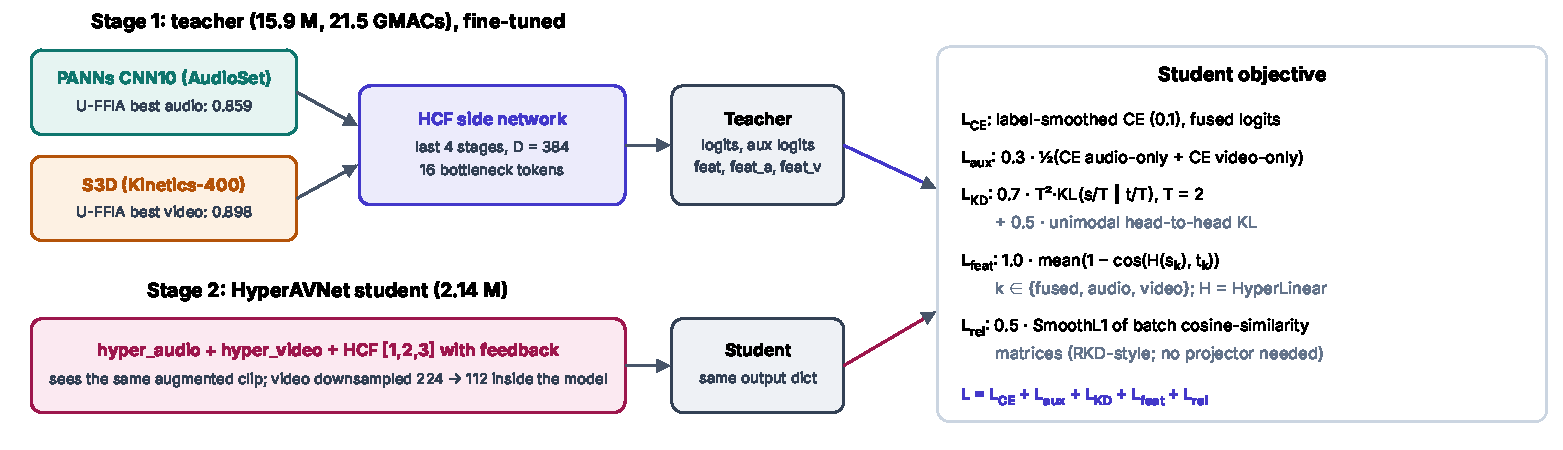
\includegraphics[width=0.92\textwidth]{figures/distillation.pdf}
  \caption{Two-stage training. A teacher built from pretrained audio and video backbones and HCF fusion
  is trained first and frozen. The HyperAVNet student is then trained with the supervised loss plus
  logit-, embedding- and relation-level distillation (Eq.~\eqref{eq:total}).}
  \label{fig:distill}
\end{figure*}

\subsection{Complexity}
\label{sec:complexity}
By Eq.~\eqref{eq:params}, every hypercomplex projection stores $1/n$ of the real parameters. Only the
stems, the depth-wise convolutions, normalisation layers and the final $4$-way classifier stay real.
For the default student ($n=4$), the network has 2.14\,M parameters against 7.88\,M for the identical
real network ($n=1$), and 1.24\,M (octonion) or 0.78\,M (sedenion) for higher algebras. Compute is
1.18\,GMACs per clip for every $n$ (16 frames at $112^{2}$ and 2\,s of audio). The added cost of a
fusion stage is about 0.17\,M parameters and under 0.02\,GMACs.
 in any paper.
%  Requires: amsmath, amssymb, bm, booktabs, graphicx, (cleveref optional).
% ============================================================================
\section{Methodology}
\label{sec:method}

\subsection{Problem formulation}
\label{sec:problem}
Each sample of AV-FFIA is a synchronised two-second clip $(\mathbf{x}^{a}, \mathbf{X}^{v})$, where
$\mathbf{x}^{a}\in\mathbb{R}^{L}$ is the hydrophone waveform ($L = 2f_s$, $f_s = 64$\,kHz) and
$\mathbf{X}^{v}\in[0,1]^{3\times T\times H\times W}$ holds $T$ RGB frames sampled uniformly from the
overhead camera. The label $y\in\mathcal{Y}=\{\textsc{None},\textsc{Weak},\textsc{Medium},\textsc{Strong}\}$
is the feeding intensity. We learn $f_{\theta}:(\mathbf{x}^{a},\mathbf{X}^{v})\mapsto\mathbf{p}\in\Delta^{|\mathcal{Y}|-1}$ with
two goals that pull in opposite directions: high accuracy, robust to the acoustic and visual
corruptions typical of aquaculture (bubbles, pumps, low light, reflections), and a small
parameter and compute budget for on-site deployment.

HyperAVNet (Fig.~\ref{fig:overview}) has four parts. Two hypercomplex backbones map each modality to a
hierarchy of \emph{stage tokens} (Sec.~\ref{sec:backbones}). A set of shared \emph{bottleneck tokens}
is updated by hypercomplex component fusion (HCF) blocks attached at a configurable subset of
stages, with zero-initialised cross-modal feedback into both streams (Secs.~\ref{sec:hcf},~\ref{sec:schedule}).
Fused and unimodal heads produce the predictions (Sec.~\ref{sec:heads}). The model is trained with a
multi-level distillation objective from a pretrained audio-visual teacher (Sec.~\ref{sec:objective}).

\begin{figure*}[t]
  \centering
  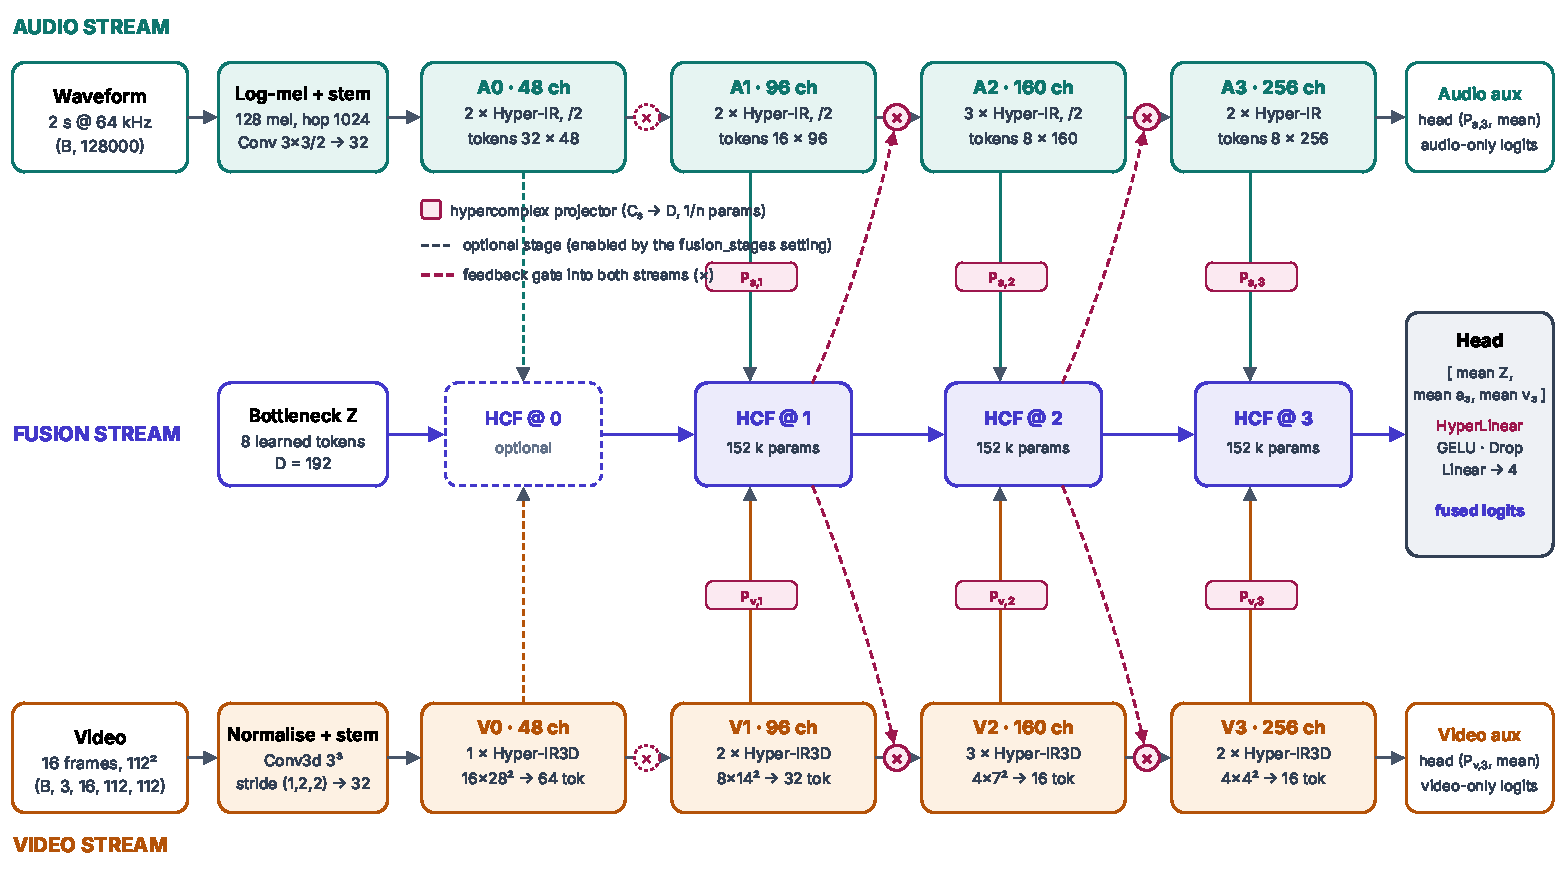
\includegraphics[width=\textwidth]{figures/arch_overview.pdf}
  \caption{HyperAVNet (default configuration: quaternion algebra, fusion stages $\mathcal{S}=\{1,2,3\}$,
  feedback enabled). Stage tokens of the audio and video backbones are projected by hypercomplex
  projectors $P_{a,s}$ and $P_{v,s}$ into a $D$-dimensional fusion space, where HCF blocks update the
  bottleneck tokens $\mathbf{Z}$. After each fused stage $s<S-1$, a zero-initialised gate ($\times$)
  modulates both streams. The classifier reads the pooled bottleneck and the pooled last-stage
  tokens; auxiliary heads supervise each modality on its own. Token shapes are for one 2\,s clip and
  $16\times112^{2}$ frames.}
  \label{fig:overview}
\end{figure*}

\subsection{Hypercomplex layers}
\label{sec:hyper}
Let $\mathbb{A}_n$ be a hypercomplex algebra of dimension $n\in\{2,4,8,16\}$ (complex numbers,
quaternions, octonions, sedenions, obtained by the Cayley--Dickson construction), with basis
$\{e_0,\dots,e_{n-1}\}$ and multiplication table
\begin{equation}
  e_i\,e_j = \sigma_{ij}\, e_{\pi(i,j)},
  \label{eq:table}
\end{equation}
with signs $\sigma_{ij}\in\{-1,+1\}$ and indices $\pi(i,j)\in\{0,\dots,n-1\}$.
A feature vector $\mathbf{x}\in\mathbb{R}^{d_{\mathrm{in}}}$ is split into $n$ components,
$\mathbf{x}=[\mathbf{x}_0;\dots;\mathbf{x}_{n-1}]$ with $\mathbf{x}_j\in\mathbb{R}^{d_{\mathrm{in}}/n}$,
i.e.\ it is read as $\sum_j \mathbf{x}_j e_j$. A hypercomplex weight
$\mathbf{W}=\sum_{k}\mathbf{W}_k e_k$ with real blocks $\mathbf{W}_k\in\mathbb{R}^{(d_{\mathrm{out}}/n)\times(d_{\mathrm{in}}/n)}$
acts on it by the algebra product, which in matrix form is
\begin{equation}
\begin{gathered}
  \mathbf{y}_i = \sum_{j=0}^{n-1} s_{ij}\,\mathbf{W}_{c(i,j)}\,\mathbf{x}_j + \mathbf{b}_i,\\
  \mathbf{K}(\mathbf{W}) = \big[\, s_{ij}\,\mathbf{W}_{c(i,j)} \,\big]_{i,j=0}^{n-1}\in\mathbb{R}^{d_{\mathrm{out}}\times d_{\mathrm{in}}},
\end{gathered}
  \label{eq:hlinear}
\end{equation}
where the block index $c(i,j)$ and sign $s_{ij}$ follow from Eq.~\eqref{eq:table}. For quaternions the
kernel takes the familiar Hamilton form (Fig.~\ref{fig:hamilton}),
\begin{equation}
  \mathbf{K} = \begin{bmatrix}
   \mathbf{W}_0 & \mathbf{W}_1 & \mathbf{W}_2 & \mathbf{W}_3\\
  -\mathbf{W}_1 & \mathbf{W}_0 & \mathbf{W}_3 & -\mathbf{W}_2\\
  -\mathbf{W}_2 & -\mathbf{W}_3 & \mathbf{W}_0 & \mathbf{W}_1\\
  -\mathbf{W}_3 & \mathbf{W}_2 & -\mathbf{W}_1 & \mathbf{W}_0
  \end{bmatrix}.
  \label{eq:hamilton}
\end{equation}
Every output component is thus a signed combination of \emph{every} input component through one
shared set of $n$ blocks, so the layer has
\begin{equation}
  |\theta_{\mathrm{hyper}}| = \tfrac{1}{n}\,d_{\mathrm{in}}d_{\mathrm{out}} + d_{\mathrm{out}}
  \;\;\text{vs.}\;\;
  |\theta_{\mathrm{real}}| = d_{\mathrm{in}}d_{\mathrm{out}} + d_{\mathrm{out}}
  \label{eq:params}
\end{equation}
parameters. A hypercomplex convolution applies the same block structure to the kernel tensor, with
$\mathbf{W}_k\in\mathbb{R}^{(C_{\mathrm{out}}/n)\times(C_{\mathrm{in}}/n)\times k_1\times\dots}$.
Weights are initialised in polar form: a modulus drawn from a $\chi$ distribution with $n$ degrees of
freedom (scaled by the Glorot variance), a uniform phase, and a unit-norm imaginary direction
\cite{bojesomo2024hypercomplex}. We write $\mathcal{H}_n(\cdot)$ for a hypercomplex linear or
convolutional layer. With $n=1$ it reduces to the real layer, which gives a matched real-valued
ablation with an identical code path.

\paragraph{Deployment.} Building $\mathbf{K}$ in Eq.~\eqref{eq:hlinear} at every forward pass
is only needed while training. After training, every $\mathcal{H}_n$ is \emph{reparameterised} into a
dense layer with weight $\mathbf{K}(\mathbf{W})$. The outputs are identical, and the run-time
overhead of kernel assembly disappears. The hypercomplex structure therefore reduces the number of
stored and optimised parameters (and the model's memory and transmission size) by up to $n\times$,
but \emph{not} the multiply--accumulate count, because $\mathbf{K}$ is dense.

\begin{figure}[t]
  \centering
  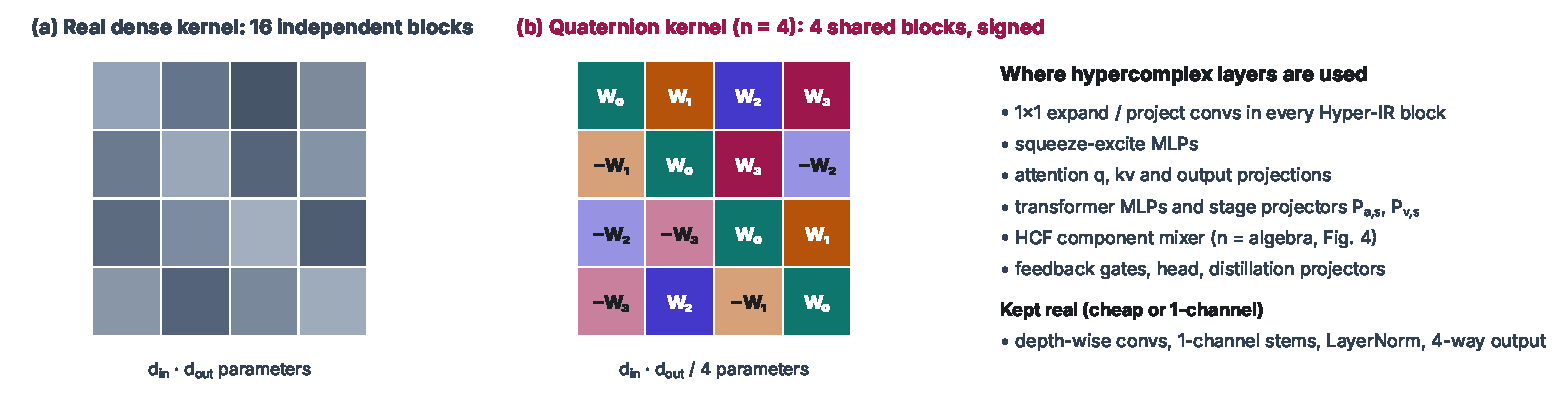
\includegraphics[width=\columnwidth]{figures/hamilton.pdf}
  \caption{Hamilton-product weight sharing. (a) A real kernel has $n^{2}$ independent blocks.
  (b) A quaternion kernel ($n=4$) re-uses four blocks with fixed signs (Eq.~\eqref{eq:hamilton}),
  which cuts the parameter count by $4\times$.}
  \label{fig:hamilton}
\end{figure}

\subsection{Hypercomplex backbones and stage tokens}
\label{sec:backbones}
\paragraph{Hyper-IR block.} Both backbones stack hypercomplex inverted-residual blocks
(Fig.~\ref{fig:hyperir}). For an input $\mathbf{h}\in\mathbb{R}^{C\times\Omega}$ ($\Omega$ is the 2-D
time--frequency grid for audio and the 3-D space--time grid for video) and expansion ratio $r=4$:
\begin{equation}
\begin{aligned}
  \mathbf{u} &= \operatorname{SiLU}\big(\operatorname{BN}(\mathcal{H}_n^{1\times1}(\mathbf{h}))\big)\in\mathbb{R}^{rC\times\Omega},\\
  \mathbf{v} &= \operatorname{SiLU}\big(\operatorname{BN}(\operatorname{DWConv}_{3}(\mathbf{u}))\big),\\
  \mathbf{w} &= \mathbf{v}\odot\sigma\big(\mathcal{H}_n(\operatorname{SiLU}(\mathcal{H}_n(\operatorname{GAP}(\mathbf{v}))))\big),\\
  \mathbf{h}' &= \mathbf{h} + \operatorname{DropPath}\big(\operatorname{BN}(\mathcal{H}_n^{1\times1}(\mathbf{w}))\big).
\end{aligned}
  \label{eq:hyperir}
\end{equation}
The two point-wise convolutions hold almost all of a block's parameters, so they are hypercomplex. The
depth-wise convolution stays real; it accounts for about 1\% of the parameters. The residual is used
when the shape is preserved.

\paragraph{Audio stream.} The waveform is converted to a log-mel spectrogram with the U-FFIA settings
(Hann window 2048, hop 1024, 128 mel bins at 64\,kHz, so a 2\,s clip gives $128\times126$),
normalised per mel bin by batch normalisation and augmented with SpecAugment during training. A
$3{\times}3$ stride-2 stem is followed by four Hyper-IR stages $s=0,\dots,3$ with widths
$(48,96,160,256)$ and depths $(2,2,3,2)$. A stage map $\mathbf{h}^{a}_{s}\in\mathbb{R}^{C_s\times T_s\times F_s}$
becomes time tokens by pooling over frequency:
\begin{equation}
  \mathbf{a}_s = \big[\operatorname{mean}_{F}(\mathbf{h}^{a}_s) + \operatorname{max}_{F}(\mathbf{h}^{a}_s)\big]^{\top}\in\mathbb{R}^{T_s\times C_s}.
  \label{eq:audiotokens}
\end{equation}
The max term keeps the short impulsive transients of feeding (chewing, tail slaps).

\paragraph{Video stream.} The frames are normalised and passed through a $3{\times}3{\times}3$ stem
(spatial stride 2) and four 3-D Hyper-IR stages of the same widths, with depths $(1,2,3,2)$ and
strides $(1,2,2)$, $(2,2,2)$, $(2,2,2)$, $(1,2,2)$. A stage map
$\mathbf{h}^{v}_{s}\in\mathbb{R}^{C_s\times T_s\times H_s\times W_s}$ is pooled to a $2\times2$ spatial grid
per time step, $\mathbf{v}_s\in\mathbb{R}^{4T_s\times C_s}$. This keeps coarse location (where the fish
aggregate) at a small token count.

\begin{figure}[t]
  \centering
  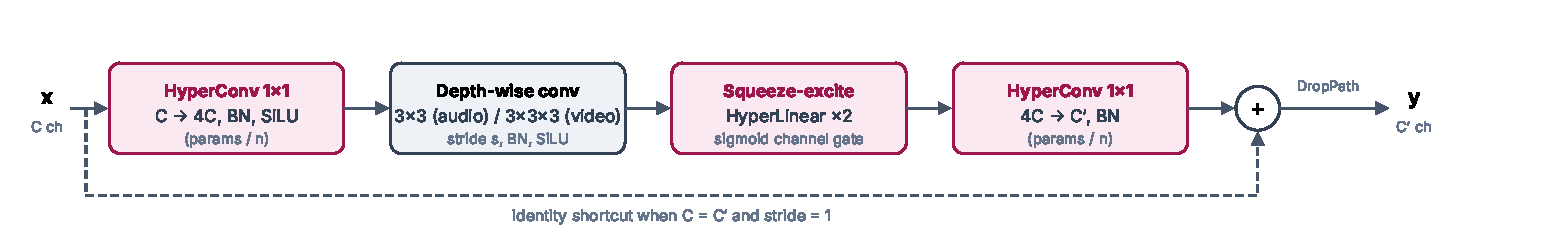
\includegraphics[width=\columnwidth]{figures/hyper_ir.pdf}
  \caption{Hypercomplex inverted-residual (Hyper-IR) block, Eq.~\eqref{eq:hyperir}. Hypercomplex
  layers are shaded; the depth-wise convolution is real.}
  \label{fig:hyperir}
\end{figure}

\paragraph{Pretrained backbones.} Any pretrained network can replace a student backbone if it exposes
four stages in the same token format. We use this for the teachers and for the teacher ablation
(Sec.~\ref{sec:setup}): PANNs CNN10/CNN14~\cite{kong2020panns}, EfficientAT~\cite{schmid2023efficientat},
AST~\cite{gong2021ast}, S3D~\cite{xie2018s3d}, X3D~\cite{feichtenhofer2020x3d},
MoViNet~\cite{kondratyuk2021movinets} and VideoMAE~\cite{tong2022videomae}. Their intermediate layers
supply the stage tokens.

\subsection{Hypercomplex component fusion}
\label{sec:hcf}
\paragraph{Projection.} Stage tokens are mapped into a shared $D$-dimensional space by hypercomplex
projectors with a learned modality embedding:
\begin{equation}
  \mathbf{A}_s = \operatorname{LN}\!\big(\mathcal{H}_n(\mathbf{a}_s)\big) + \mathbf{m}^{a},\qquad
  \mathbf{V}_s = \operatorname{LN}\!\big(\mathcal{H}_n(\mathbf{v}_s)\big) + \mathbf{m}^{v}.
  \label{eq:proj}
\end{equation}

\paragraph{Bottleneck state.} The fused representation lives in $N_b$ learned bottleneck tokens
$\mathbf{Z}\in\mathbb{R}^{N_b\times D}$ (we use $N_b=8$, $D=192$), shared across stages.

\paragraph{HCF block.} At a fusion stage $s$, the bottleneck first reads each modality with its own
hypercomplex cross-attention:
\begin{equation}
\begin{aligned}
  \mathbf{Z}^{a} &= \mathbf{Z} + \operatorname{XAttn}_{n}\big(\operatorname{LN}\mathbf{Z},\,\operatorname{LN}\mathbf{A}_s\big),\\
  \mathbf{Z}^{v} &= \mathbf{Z} + \operatorname{XAttn}_{n}\big(\operatorname{LN}\mathbf{Z},\,\operatorname{LN}\mathbf{V}_s\big),
\end{aligned}
  \label{eq:xattn}
\end{equation}
where $\operatorname{XAttn}_n$ is multi-head attention whose query, key, value and output projections
are hypercomplex (shown for one head of width $d_h$):
\begin{equation*}
  \operatorname{XAttn}_n(\mathbf{Q},\mathbf{C})=\mathcal{H}_n\Big(\operatorname{softmax}\Big(\tfrac{\mathcal{H}_n(\mathbf{Q})\,\mathcal{H}_n(\mathbf{C})^{\top}}{\sqrt{d_h}}\Big)\mathcal{H}_n(\mathbf{C})\Big).
\end{equation*} The shared
state, the two modality views and their interaction then form the components of one element of
$\mathbb{A}_m$:
\begin{equation}
  \mathbf{q} = \mathbf{Z}\,e_0 + \mathbf{Z}^{a}\,e_1 + \mathbf{Z}^{v}\,e_2 + \big(\hat{\mathbf{Z}}^{a}\odot\hat{\mathbf{Z}}^{v}\big)\,e_3,
  \label{eq:components}
\end{equation}
for $m=4$,
with $\hat{\cdot}=\operatorname{LN}(\cdot)$. The octonion variant ($m=8$) appends
$(\mathbf{Z}^{a}-\mathbf{Z}^{v})e_4$, $(\hat{\mathbf{Z}}\odot\hat{\mathbf{Z}}^{a})e_5$,
$(\hat{\mathbf{Z}}\odot\hat{\mathbf{Z}}^{v})e_6$ and
$(\hat{\mathbf{Z}}\odot\hat{\mathbf{Z}}^{a}\odot\hat{\mathbf{Z}}^{v})e_7$; the complex variant ($m=2$) uses
$(\mathbf{Z}^{a},\mathbf{Z}^{v})$. The components are mixed by a single Hamilton product, followed by a
hypercomplex MLP:
\begin{equation}
\begin{aligned}
  \mathbf{Z} &\leftarrow \mathbf{Z} + \boldsymbol{\gamma}_1\odot \mathcal{H}_m(\mathbf{q}),\\
  \mathbf{Z} &\leftarrow \mathbf{Z} + \boldsymbol{\gamma}_2\odot \operatorname{MLP}_n(\operatorname{LN}\mathbf{Z}),
\end{aligned}
  \label{eq:mix}
\end{equation}
where $\mathcal{H}_m:\mathbb{R}^{mD}\to\mathbb{R}^{D}$ is a hypercomplex linear layer of algebra
$\mathbb{A}_m$ and $\boldsymbol{\gamma}_{1,2}$ are LayerScale vectors~\cite{touvron2021cait}, initialised to
$10^{-2}$. By Eq.~\eqref{eq:hlinear}, each output component of $\mathcal{H}_m$ is a signed mixture of
the shared state, both modality views and their multiplicative agreement, all through one set of
$m$ blocks. The mixer has $D^{2}$ parameters \emph{for every} $m$, against $mD^{2}$ for a dense mixer, so
the octonion variant adds four interaction terms at no parameter cost. Unlike attention bottlenecks
that attend to the modalities one after the other~\cite{nagrani2021mbt}, HCF reads both modalities
in parallel and combines them in one algebraic product (Fig.~\ref{fig:hcf}).

\begin{figure*}[t]
  \centering
  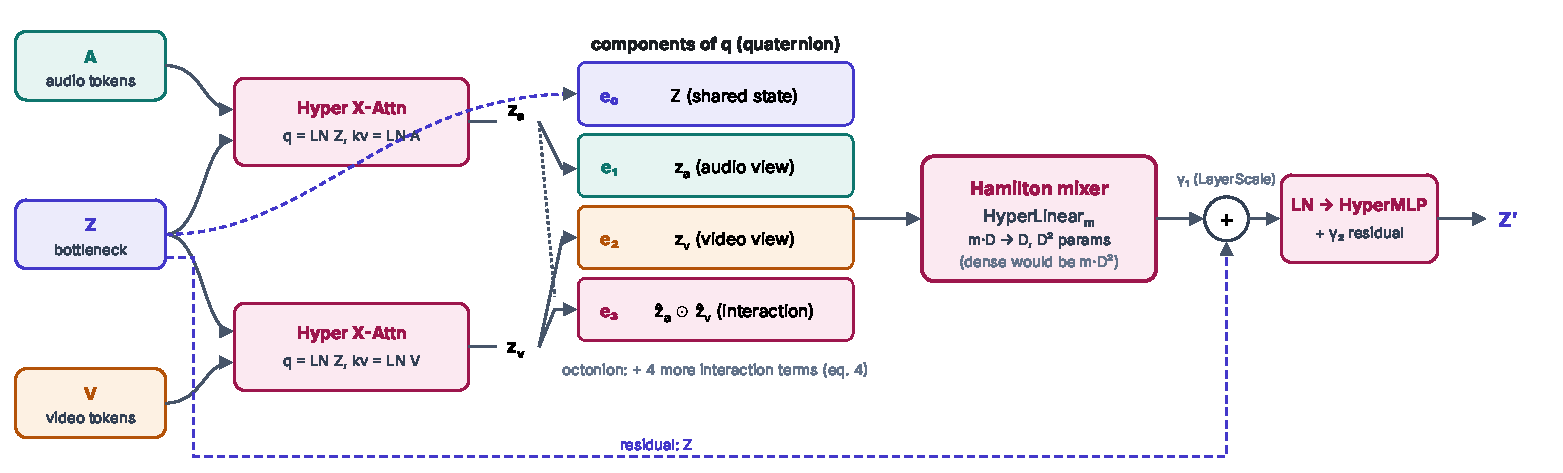
\includegraphics[width=0.9\textwidth]{figures/hcf_block.pdf}
  \caption{Hypercomplex component fusion (HCF), Eqs.~\eqref{eq:xattn}--\eqref{eq:mix}. The modality
  views and their interaction are the components of one quaternion and are mixed by a single
  Hamilton product.}
  \label{fig:hcf}
\end{figure*}

\subsection{Deep-to-early fusion schedule with cross-modal feedback}
\label{sec:schedule}
The set $\mathcal{S}\subseteq\{0,\dots,S-1\}$ selects the stages at which an HCF block is attached:
\begin{equation}
  \mathbf{Z}^{(s+1)} = \begin{cases}\operatorname{HCF}_s\big(\mathbf{Z}^{(s)},\mathbf{A}_s,\mathbf{V}_s\big), & s\in\mathcal{S},\\ \mathbf{Z}^{(s)}, & \text{otherwise,}\end{cases}
  \label{eq:schedule}
\end{equation}
with $\mathbf{Z}^{(0)}=\mathbf{Z}_{\mathrm{init}}$ the learned bottleneck tokens.
Varying $\mathcal{S}$ from $\{S-1\}$ (late fusion) through $\{S-2,S-1\}$ and so on to $\{0,\dots,S-1\}$
gives a controlled \emph{deep-to-early} study of where audio--visual fusion helps. Because the student
backbones are executed stage by stage, the fused state is also fed back into both streams after each
fused stage $s<S-1$:
\begin{equation}
  \mathbf{h}^{m}_s \leftarrow \mathbf{h}^{m}_s\odot\big(1+\tanh(\mathcal{G}^{m}_s\,\bar{\mathbf{z}}^{(s+1)})\big),\quad m\in\{a,v\},
  \label{eq:feedback}
\end{equation}
where $\bar{\mathbf{z}}=\operatorname{mean}_{N_b}(\mathbf{Z})$, the gates
$\mathcal{G}^{m}_s$ are hypercomplex linear maps $\mathbb{R}^{D}\to\mathbb{R}^{C_s}$, and the
product broadcasts over $\Omega$. The gates are \emph{initialised to zero}, so training starts exactly
at the feedback-free model. The network then learns how strongly each modality should condition the
other's later features. This is genuine early fusion, as opposed to fusing independently computed
features.

\subsection{Prediction heads and modality dropout}
\label{sec:heads}
With $\bar{\mathbf{z}}=\operatorname{mean}(\operatorname{LN}\mathbf{Z}^{(S)})$,
$\bar{\mathbf{a}}=\operatorname{mean}(\operatorname{LN}\mathbf{A}_{S-1})$ and
$\bar{\mathbf{v}}=\operatorname{mean}(\operatorname{LN}\mathbf{V}_{S-1})$, the fused and auxiliary logits are
\begin{equation}
\begin{gathered}
  \boldsymbol{\ell} = \mathbf{W}_o\,\operatorname{GELU}\big(\mathcal{H}_n[\bar{\mathbf{z}};\,\mu_a\bar{\mathbf{a}};\,\mu_v\bar{\mathbf{v}}]\big),\\
  \boldsymbol{\ell}^{a} = \mathbf{W}_a\bar{\mathbf{a}},\qquad \boldsymbol{\ell}^{v} = \mathbf{W}_v\bar{\mathbf{v}}.
\end{gathered}
  \label{eq:heads}
\end{equation}
Here $\mu_a,\mu_v\in\{0,1\}$ are per-sample modality masks. During training,
$(\mu_a,\mu_v)=(0,1)$ with probability $p$, $(1,0)$ with probability $p$, and $(1,1)$ otherwise. In the
notation of~\cite{cui2024uffia}, $p_{av}=1-2p$ and $p_a=p_v=p$. The same mask multiplies every fusion
input $\mathbf{A}_s,\mathbf{V}_s$, so a dropped modality is absent everywhere. The auxiliary heads always see
their own modality, which keeps both branches trained regardless of $p$. At test time, forcing
$\mu_a=0$ or $\mu_v=0$ evaluates the model with a missing modality.

\subsection{Training objective and multi-level distillation}
\label{sec:objective}
The supervised loss combines label-smoothed cross-entropy on the fused logits with the two
auxiliary terms:
\begin{equation}
  \mathcal{L}_{\mathrm{sup}} = \operatorname{CE}_{\epsilon}(\boldsymbol{\ell},y)
   + \tfrac{\lambda_{\mathrm{aux}}}{2}\!\!\sum_{m\in\{a,v\}}\!\!\operatorname{CE}_{\epsilon}(\boldsymbol{\ell}^{m},y).
  \label{eq:sup}
\end{equation}
A frozen teacher $g$ with the same output structure (pretrained backbones and HCF fusion) provides
three further signals. At the \emph{logit level}, with temperature $\tau$:
\begin{equation}
  \mathcal{L}_{\mathrm{KD}} = \tau^{2}\,\mathrm{KL}\big(\boldsymbol{\ell}^{g}\,\|\,\boldsymbol{\ell}\big)_{\tau}
   + \tfrac{\lambda_{u}\tau^{2}}{2}\!\!\sum_{m\in\{a,v\}}\!\!\mathrm{KL}\big(\boldsymbol{\ell}^{g,m}\,\|\,\boldsymbol{\ell}^{m}\big)_{\tau},
  \label{eq:kd}
\end{equation}
with $\mathrm{KL}(\mathbf{u}\,\|\,\mathbf{w})_{\tau}=\mathrm{KL}\big(\operatorname{softmax}(\mathbf{u}/\tau)\,\|\,\operatorname{softmax}(\mathbf{w}/\tau)\big)$,
which distils each unimodal head from its counterpart in the teacher. U-FFIA's variant~\cite{cui2024uffia}
softens only the teacher, $\mathrm{KL}(\operatorname{softmax}(\boldsymbol{\ell}^{g}/\tau)\,\|\,\operatorname{softmax}(\boldsymbol{\ell}))$,
and is evaluated as an ablation. At the \emph{embedding level}, small hypercomplex projectors
$\mathcal{P}_k$ align the student's pooled embeddings with the teacher's:
\begin{equation}
  \mathcal{L}_{\mathrm{feat}} = \tfrac{1}{3}\!\!\sum_{k\in\{\bar{\mathbf{z}},\bar{\mathbf{a}},\bar{\mathbf{v}}\}}\!\!
  \big(1-\cos(\mathcal{P}_k(k),\,k^{g})\big).
  \label{eq:feat}
\end{equation}
At the \emph{relation level}~\cite{park2019rkd}, the within-batch similarity structure of the fused
embeddings is matched:
\begin{equation}
  \mathcal{L}_{\mathrm{rel}} = \operatorname{SmoothL1}\big(\mathbf{R}(\bar{\mathbf{z}}_{1:B}),\,\mathbf{R}(\bar{\mathbf{z}}^{g}_{1:B})\big),
  \label{eq:rel}
\end{equation}
where $\mathbf{R}(\mathbf{U})_{ij}=\mathbf{u}_i^{\top}\mathbf{u}_j/(\|\mathbf{u}_i\|\|\mathbf{u}_j\|)$ is the cosine-similarity matrix of a batch of size $B$.
The full objective is
\begin{equation}
  \mathcal{L} = \mathcal{L}_{\mathrm{sup}} + \alpha\,\mathcal{L}_{\mathrm{KD}} + \beta\,\mathcal{L}_{\mathrm{feat}} + \gamma\,\mathcal{L}_{\mathrm{rel}},
  \label{eq:total}
\end{equation}
with $\epsilon=0.1$, $\lambda_{\mathrm{aux}}=0.3$, $\lambda_u=0.5$, $\tau=2$, $\alpha=0.7$, $\beta=1$ and $\gamma=0.5$.
Training proceeds in two stages: the teacher is trained with $\mathcal{L}_{\mathrm{sup}}$ and frozen, then
the student is trained with Eq.~\eqref{eq:total}.

\begin{figure*}[t]
  \centering
  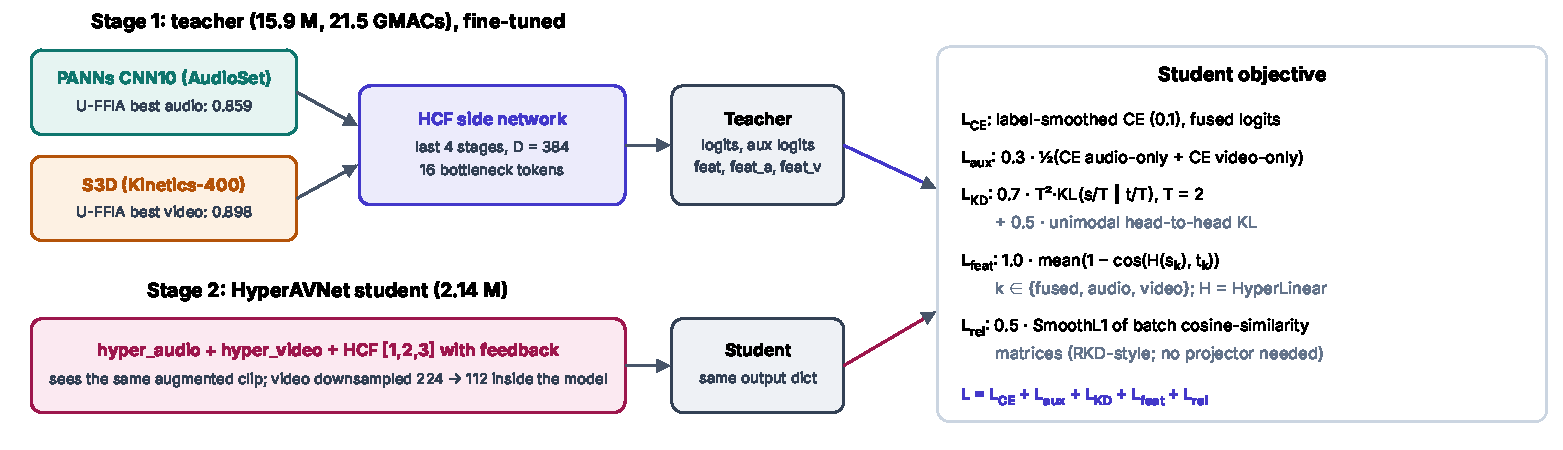
\includegraphics[width=0.92\textwidth]{figures/distillation.pdf}
  \caption{Two-stage training. A teacher built from pretrained audio and video backbones and HCF fusion
  is trained first and frozen. The HyperAVNet student is then trained with the supervised loss plus
  logit-, embedding- and relation-level distillation (Eq.~\eqref{eq:total}).}
  \label{fig:distill}
\end{figure*}

\subsection{Complexity}
\label{sec:complexity}
By Eq.~\eqref{eq:params}, every hypercomplex projection stores $1/n$ of the real parameters. Only the
stems, the depth-wise convolutions, normalisation layers and the final $4$-way classifier stay real.
For the default student ($n=4$), the network has 2.14\,M parameters against 7.88\,M for the identical
real network ($n=1$), and 1.24\,M (octonion) or 0.78\,M (sedenion) for higher algebras. Compute is
1.18\,GMACs per clip for every $n$ (16 frames at $112^{2}$ and 2\,s of audio). The added cost of a
fusion stage is about 0.17\,M parameters and under 0.02\,GMACs.

% ============================================================================
%  Experimental set-up -- % ============================================================================
%  Experimental set-up -- % ============================================================================
%  Experimental set-up -- \input{sections/experiments}
% ============================================================================
\section{Experimental Set-up}
\label{sec:setup}

\paragraph{Dataset.} AV-FFIA~\cite{cui2024uffia} contains synchronised two-second audio--video clips of
\textit{Oplegnathus punctatus} feeding in a recirculating tank, labelled by a feeding technician into
four intensities. Audio was recorded by a hydrophone at 256\,kHz (used at 64\,kHz), and video by an
overhead camera at 25\,fps. The paper describes 27,000 clips (6,750 per class). The published
splits~\cite{cui2024uffia}, later re-implementations~\cite{dynagate2026,hmmfnet2026} and the public
release disagree on the clip count, so we report the number of clips we used (\todo{N clips}) and
release our split files.

\paragraph{Evaluation protocols.} Published AV-FFIA results use incompatible protocols, so we
evaluate under three and state the protocol with every number.
(i)~\emph{Official split}: the U-FFIA rule (each class shuffled with seed 25; 700 test and 700
validation clips per class; the rest for training), applied to a \emph{sorted} file list so that the
split is deterministic. We publish its hash. This is the protocol of~\cite{cui2024uffia,dynagate2026}.
(ii)~\emph{5-fold stratified cross-validation}, as in~\cite{hmmfnet2026}; one fold is the test set, and
one-eighth of the remaining clips is held out for model selection.
(iii)~\emph{Session-disjoint split}: whole recording sessions (dates) are assigned to the train,
validation or test set. The clips are two-second segments of one-minute recordings, so every
clip-level random split, including (i) and (ii), places near-duplicate neighbours in both train and
test. Protocol (iii) measures generalisation to unseen sessions; to our knowledge it is the first
leakage-free result on AV-FFIA.

\paragraph{Pre-processing and augmentation.} Audio is resampled to 64\,kHz and cropped or padded to 2\,s.
Log-mel spectrograms follow U-FFIA (window 2048, hop 1024, 128 bins). Training uses SpecAugment
(two frequency masks of width $\le8$ and two time masks of width $\le16$), random gain
($\pm6$\,dB) and circular time shift. Sixteen frames are sampled uniformly per clip and resized to a
short side of 128 (student) or 256 (teacher), then randomly cropped to $112^{2}$ (student) or $224^{2}$
(teacher), with horizontal flips and brightness/contrast jitter. Evaluation uses a centre crop and no
augmentation. Under distillation the student receives the teacher's $224^{2}$ input and resizes it to
$112^{2}$ internally, so both models see exactly the same augmented clip.

\paragraph{Teachers.} The default teacher pairs the strongest pretrained single-modality models on
AV-FFIA~\cite{cui2024uffia}: AudioSet PANNs CNN10~\cite{kong2020panns} and Kinetics-400
S3D~\cite{xie2018s3d}. Their last four stages are fused by HCF ($\mathcal{S}=\{0,1,2,3\}$, $D=384$,
$N_b=16$), giving 15.9\,M parameters and 21.5\,GMACs. The teacher ablation (Table~\ref{tab:teachers})
varies the backbone pair over ten configurations (T1--T10), changing one modality at a time where
possible:
\begin{itemize}
  \item \emph{audio}: CNN10, CNN14, an ImageNet EfficientNet-B0 on mel spectrograms, AST~\cite{gong2021ast}, and EfficientAT
mn10~\cite{schmid2023efficientat};
  \item \emph{video}: S3D, R(2+1)D-18, a per-frame ConvNeXt-T with a hypercomplex temporal adapter,
X3D-M~\cite{feichtenhofer2020x3d}, VideoMAE-B~\cite{tong2022videomae}, and MoViNet-A0~\cite{kondratyuk2021movinets}.
\end{itemize}
T10 reproduces the EfficientAT + MoViNet-A0 teacher pair of~\cite{hmkd2026}. Each teacher is trained with
the same recipe, and a student is distilled from each.

\paragraph{Student variants.} HyperAVNet-Q is the fully hypercomplex student of Sec.~\ref{sec:method},
trained from scratch. HyperAVNet-P keeps the hypercomplex projectors, HCF fusion and heads, but replaces
the student backbones with compact pretrained networks: EfficientAT mn04~\cite{schmid2023efficientat} for
audio and MoViNet-A0~\cite{kondratyuk2021movinets} for video at $172^{2}$. This gives 1.89\,M parameters
and 0.88\,GMACs, and tests how much of the gap to the teacher is due to pretraining rather than
architecture.

\paragraph{Baselines.} We compare against the results published by
\cite{cui2024uffia,acafnet2025,dynagate2026,hmmfnet2026,hmkd2026,ldmf2026}, each with its stated protocol,
and against models we re-train under our protocol: a real-valued late-concatenation model with the
teacher's backbones, the teachers, and HyperAVNet without distillation. Re-runs of the same
cross-attention baseline in different works vary by about 1.5 percentage points (91.7\%~\cite{cui2024uffia},
92.4\%~\cite{dynagate2026}, 93.4\%~\cite{acafnet2025}). We therefore regard differences of that size
across papers as inconclusive, and draw conclusions only from comparisons within our own pipeline.

\paragraph{Implementation details.} Models are trained with AdamW ($\beta=(0.9,0.999)$, weight decay
0.05, none on normalisation, bias and token parameters), batch size 32 (student) or 16 (teacher), and a
peak learning rate of $10^{-3}$ (student) or $3\times10^{-4}$ (teacher; pretrained weights at
$0.3\times$). The schedule is a cosine decay with a two-epoch warm-up over 40 (student) or 30
(teacher) epochs. We use bf16 mixed precision, gradient clipping at 5, stochastic depth 0.1 and modality
dropout $p=0.1$. Model selection uses validation accuracy of an exponential moving average of the
weights (decay 0.999), and the test set is evaluated once. Every configuration is run with three
seeds (the split is fixed), and we report mean $\pm$ standard deviation. Parameters are counted from
the trained model. Compute is counted with PyTorch's \texttt{FlopCounterMode} and reported in MACs
(1\,MAC $=$ 2\,FLOPs), which is the unit U-FFIA calls ``FLOPs''. We confirmed this by measuring
torchvision S3D at $20\times224^{2}$ as 22.4\,GMACs, against 22.8 reported in~\cite{cui2024uffia}.

\paragraph{Metrics and robustness protocol.} We report accuracy (the standard metric in FFIA) and
macro-F1, plus audio-only and video-only accuracy from the auxiliary heads. Robustness follows
\cite{cui2024uffia}: noise is added to the whole audio clip at an SNR of $-10$, $-5$, $0$, $10$ or 20\,dB,
using bubble and pump recordings (\todo{or white noise if the recordings are unavailable; state
which}). Video is corrupted by darkness (intensities $\times0.25$) and additive Gaussian noise
($\sigma^{2}=0.2$). We also evaluate with the audio or the video absent ($\mu_a=0$ or $\mu_v=0$ in
Eq.~\eqref{eq:heads}). All corruptions are seeded, so every model sees identical corrupted inputs.

% ============================================================================
\section{Experimental Set-up}
\label{sec:setup}

\paragraph{Dataset.} AV-FFIA~\cite{cui2024uffia} contains synchronised two-second audio--video clips of
\textit{Oplegnathus punctatus} feeding in a recirculating tank, labelled by a feeding technician into
four intensities. Audio was recorded by a hydrophone at 256\,kHz (used at 64\,kHz), and video by an
overhead camera at 25\,fps. The paper describes 27,000 clips (6,750 per class). The published
splits~\cite{cui2024uffia}, later re-implementations~\cite{dynagate2026,hmmfnet2026} and the public
release disagree on the clip count, so we report the number of clips we used (\todo{N clips}) and
release our split files.

\paragraph{Evaluation protocols.} Published AV-FFIA results use incompatible protocols, so we
evaluate under three and state the protocol with every number.
(i)~\emph{Official split}: the U-FFIA rule (each class shuffled with seed 25; 700 test and 700
validation clips per class; the rest for training), applied to a \emph{sorted} file list so that the
split is deterministic. We publish its hash. This is the protocol of~\cite{cui2024uffia,dynagate2026}.
(ii)~\emph{5-fold stratified cross-validation}, as in~\cite{hmmfnet2026}; one fold is the test set, and
one-eighth of the remaining clips is held out for model selection.
(iii)~\emph{Session-disjoint split}: whole recording sessions (dates) are assigned to the train,
validation or test set. The clips are two-second segments of one-minute recordings, so every
clip-level random split, including (i) and (ii), places near-duplicate neighbours in both train and
test. Protocol (iii) measures generalisation to unseen sessions; to our knowledge it is the first
leakage-free result on AV-FFIA.

\paragraph{Pre-processing and augmentation.} Audio is resampled to 64\,kHz and cropped or padded to 2\,s.
Log-mel spectrograms follow U-FFIA (window 2048, hop 1024, 128 bins). Training uses SpecAugment
(two frequency masks of width $\le8$ and two time masks of width $\le16$), random gain
($\pm6$\,dB) and circular time shift. Sixteen frames are sampled uniformly per clip and resized to a
short side of 128 (student) or 256 (teacher), then randomly cropped to $112^{2}$ (student) or $224^{2}$
(teacher), with horizontal flips and brightness/contrast jitter. Evaluation uses a centre crop and no
augmentation. Under distillation the student receives the teacher's $224^{2}$ input and resizes it to
$112^{2}$ internally, so both models see exactly the same augmented clip.

\paragraph{Teachers.} The default teacher pairs the strongest pretrained single-modality models on
AV-FFIA~\cite{cui2024uffia}: AudioSet PANNs CNN10~\cite{kong2020panns} and Kinetics-400
S3D~\cite{xie2018s3d}. Their last four stages are fused by HCF ($\mathcal{S}=\{0,1,2,3\}$, $D=384$,
$N_b=16$), giving 15.9\,M parameters and 21.5\,GMACs. The teacher ablation (Table~\ref{tab:teachers})
varies the backbone pair over ten configurations (T1--T10), changing one modality at a time where
possible:
\begin{itemize}
  \item \emph{audio}: CNN10, CNN14, an ImageNet EfficientNet-B0 on mel spectrograms, AST~\cite{gong2021ast}, and EfficientAT
mn10~\cite{schmid2023efficientat};
  \item \emph{video}: S3D, R(2+1)D-18, a per-frame ConvNeXt-T with a hypercomplex temporal adapter,
X3D-M~\cite{feichtenhofer2020x3d}, VideoMAE-B~\cite{tong2022videomae}, and MoViNet-A0~\cite{kondratyuk2021movinets}.
\end{itemize}
T10 reproduces the EfficientAT + MoViNet-A0 teacher pair of~\cite{hmkd2026}. Each teacher is trained with
the same recipe, and a student is distilled from each.

\paragraph{Student variants.} HyperAVNet-Q is the fully hypercomplex student of Sec.~\ref{sec:method},
trained from scratch. HyperAVNet-P keeps the hypercomplex projectors, HCF fusion and heads, but replaces
the student backbones with compact pretrained networks: EfficientAT mn04~\cite{schmid2023efficientat} for
audio and MoViNet-A0~\cite{kondratyuk2021movinets} for video at $172^{2}$. This gives 1.89\,M parameters
and 0.88\,GMACs, and tests how much of the gap to the teacher is due to pretraining rather than
architecture.

\paragraph{Baselines.} We compare against the results published by
\cite{cui2024uffia,acafnet2025,dynagate2026,hmmfnet2026,hmkd2026,ldmf2026}, each with its stated protocol,
and against models we re-train under our protocol: a real-valued late-concatenation model with the
teacher's backbones, the teachers, and HyperAVNet without distillation. Re-runs of the same
cross-attention baseline in different works vary by about 1.5 percentage points (91.7\%~\cite{cui2024uffia},
92.4\%~\cite{dynagate2026}, 93.4\%~\cite{acafnet2025}). We therefore regard differences of that size
across papers as inconclusive, and draw conclusions only from comparisons within our own pipeline.

\paragraph{Implementation details.} Models are trained with AdamW ($\beta=(0.9,0.999)$, weight decay
0.05, none on normalisation, bias and token parameters), batch size 32 (student) or 16 (teacher), and a
peak learning rate of $10^{-3}$ (student) or $3\times10^{-4}$ (teacher; pretrained weights at
$0.3\times$). The schedule is a cosine decay with a two-epoch warm-up over 40 (student) or 30
(teacher) epochs. We use bf16 mixed precision, gradient clipping at 5, stochastic depth 0.1 and modality
dropout $p=0.1$. Model selection uses validation accuracy of an exponential moving average of the
weights (decay 0.999), and the test set is evaluated once. Every configuration is run with three
seeds (the split is fixed), and we report mean $\pm$ standard deviation. Parameters are counted from
the trained model. Compute is counted with PyTorch's \texttt{FlopCounterMode} and reported in MACs
(1\,MAC $=$ 2\,FLOPs), which is the unit U-FFIA calls ``FLOPs''. We confirmed this by measuring
torchvision S3D at $20\times224^{2}$ as 22.4\,GMACs, against 22.8 reported in~\cite{cui2024uffia}.

\paragraph{Metrics and robustness protocol.} We report accuracy (the standard metric in FFIA) and
macro-F1, plus audio-only and video-only accuracy from the auxiliary heads. Robustness follows
\cite{cui2024uffia}: noise is added to the whole audio clip at an SNR of $-10$, $-5$, $0$, $10$ or 20\,dB,
using bubble and pump recordings (\todo{or white noise if the recordings are unavailable; state
which}). Video is corrupted by darkness (intensities $\times0.25$) and additive Gaussian noise
($\sigma^{2}=0.2$). We also evaluate with the audio or the video absent ($\mu_a=0$ or $\mu_v=0$ in
Eq.~\eqref{eq:heads}). All corruptions are seeded, so every model sees identical corrupted inputs.

% ============================================================================
\section{Experimental Set-up}
\label{sec:setup}

\paragraph{Dataset.} AV-FFIA~\cite{cui2024uffia} contains synchronised two-second audio--video clips of
\textit{Oplegnathus punctatus} feeding in a recirculating tank, labelled by a feeding technician into
four intensities. Audio was recorded by a hydrophone at 256\,kHz (used at 64\,kHz), and video by an
overhead camera at 25\,fps. The paper describes 27,000 clips (6,750 per class). The published
splits~\cite{cui2024uffia}, later re-implementations~\cite{dynagate2026,hmmfnet2026} and the public
release disagree on the clip count, so we report the number of clips we used (\todo{N clips}) and
release our split files.

\paragraph{Evaluation protocols.} Published AV-FFIA results use incompatible protocols, so we
evaluate under three and state the protocol with every number.
(i)~\emph{Official split}: the U-FFIA rule (each class shuffled with seed 25; 700 test and 700
validation clips per class; the rest for training), applied to a \emph{sorted} file list so that the
split is deterministic. We publish its hash. This is the protocol of~\cite{cui2024uffia,dynagate2026}.
(ii)~\emph{5-fold stratified cross-validation}, as in~\cite{hmmfnet2026}; one fold is the test set, and
one-eighth of the remaining clips is held out for model selection.
(iii)~\emph{Session-disjoint split}: whole recording sessions (dates) are assigned to the train,
validation or test set. The clips are two-second segments of one-minute recordings, so every
clip-level random split, including (i) and (ii), places near-duplicate neighbours in both train and
test. Protocol (iii) measures generalisation to unseen sessions; to our knowledge it is the first
leakage-free result on AV-FFIA.

\paragraph{Pre-processing and augmentation.} Audio is resampled to 64\,kHz and cropped or padded to 2\,s.
Log-mel spectrograms follow U-FFIA (window 2048, hop 1024, 128 bins). Training uses SpecAugment
(two frequency masks of width $\le8$ and two time masks of width $\le16$), random gain
($\pm6$\,dB) and circular time shift. Sixteen frames are sampled uniformly per clip and resized to a
short side of 128 (student) or 256 (teacher), then randomly cropped to $112^{2}$ (student) or $224^{2}$
(teacher), with horizontal flips and brightness/contrast jitter. Evaluation uses a centre crop and no
augmentation. Under distillation the student receives the teacher's $224^{2}$ input and resizes it to
$112^{2}$ internally, so both models see exactly the same augmented clip.

\paragraph{Teachers.} The default teacher pairs the strongest pretrained single-modality models on
AV-FFIA~\cite{cui2024uffia}: AudioSet PANNs CNN10~\cite{kong2020panns} and Kinetics-400
S3D~\cite{xie2018s3d}. Their last four stages are fused by HCF ($\mathcal{S}=\{0,1,2,3\}$, $D=384$,
$N_b=16$), giving 15.9\,M parameters and 21.5\,GMACs. The teacher ablation (Table~\ref{tab:teachers})
varies the backbone pair over ten configurations (T1--T10), changing one modality at a time where
possible:
\begin{itemize}
  \item \emph{audio}: CNN10, CNN14, an ImageNet EfficientNet-B0 on mel spectrograms, AST~\cite{gong2021ast}, and EfficientAT
mn10~\cite{schmid2023efficientat};
  \item \emph{video}: S3D, R(2+1)D-18, a per-frame ConvNeXt-T with a hypercomplex temporal adapter,
X3D-M~\cite{feichtenhofer2020x3d}, VideoMAE-B~\cite{tong2022videomae}, and MoViNet-A0~\cite{kondratyuk2021movinets}.
\end{itemize}
T10 reproduces the EfficientAT + MoViNet-A0 teacher pair of~\cite{hmkd2026}. Each teacher is trained with
the same recipe, and a student is distilled from each.

\paragraph{Student variants.} HyperAVNet-Q is the fully hypercomplex student of Sec.~\ref{sec:method},
trained from scratch. HyperAVNet-P keeps the hypercomplex projectors, HCF fusion and heads, but replaces
the student backbones with compact pretrained networks: EfficientAT mn04~\cite{schmid2023efficientat} for
audio and MoViNet-A0~\cite{kondratyuk2021movinets} for video at $172^{2}$. This gives 1.89\,M parameters
and 0.88\,GMACs, and tests how much of the gap to the teacher is due to pretraining rather than
architecture.

\paragraph{Baselines.} We compare against the results published by
\cite{cui2024uffia,acafnet2025,dynagate2026,hmmfnet2026,hmkd2026,ldmf2026}, each with its stated protocol,
and against models we re-train under our protocol: a real-valued late-concatenation model with the
teacher's backbones, the teachers, and HyperAVNet without distillation. Re-runs of the same
cross-attention baseline in different works vary by about 1.5 percentage points (91.7\%~\cite{cui2024uffia},
92.4\%~\cite{dynagate2026}, 93.4\%~\cite{acafnet2025}). We therefore regard differences of that size
across papers as inconclusive, and draw conclusions only from comparisons within our own pipeline.

\paragraph{Implementation details.} Models are trained with AdamW ($\beta=(0.9,0.999)$, weight decay
0.05, none on normalisation, bias and token parameters), batch size 32 (student) or 16 (teacher), and a
peak learning rate of $10^{-3}$ (student) or $3\times10^{-4}$ (teacher; pretrained weights at
$0.3\times$). The schedule is a cosine decay with a two-epoch warm-up over 40 (student) or 30
(teacher) epochs. We use bf16 mixed precision, gradient clipping at 5, stochastic depth 0.1 and modality
dropout $p=0.1$. Model selection uses validation accuracy of an exponential moving average of the
weights (decay 0.999), and the test set is evaluated once. Every configuration is run with three
seeds (the split is fixed), and we report mean $\pm$ standard deviation. Parameters are counted from
the trained model. Compute is counted with PyTorch's \texttt{FlopCounterMode} and reported in MACs
(1\,MAC $=$ 2\,FLOPs), which is the unit U-FFIA calls ``FLOPs''. We confirmed this by measuring
torchvision S3D at $20\times224^{2}$ as 22.4\,GMACs, against 22.8 reported in~\cite{cui2024uffia}.

\paragraph{Metrics and robustness protocol.} We report accuracy (the standard metric in FFIA) and
macro-F1, plus audio-only and video-only accuracy from the auxiliary heads. Robustness follows
\cite{cui2024uffia}: noise is added to the whole audio clip at an SNR of $-10$, $-5$, $0$, $10$ or 20\,dB,
using bubble and pump recordings (\todo{or white noise if the recordings are unavailable; state
which}). Video is corrupted by darkness (intensities $\times0.25$) and additive Gaussian noise
($\sigma^{2}=0.2$). We also evaluate with the audio or the video absent ($\mu_a=0$ or $\mu_v=0$ in
Eq.~\eqref{eq:heads}). All corruptions are seeded, so every model sees identical corrupted inputs.

% ============================================================================
%  Results -- % ============================================================================
%  Results -- % ============================================================================
%  Results -- \input{sections/results}
%  Numbers come from tables/*.tex and tables/macros.tex, generated by
%  scripts/make_paper_assets.py from the run folders. Re-run it after new runs.
%  Sentences marked \todo{} state a claim that must be checked against the
%  final numbers (keep, reverse or delete).
% ============================================================================
\section{Results}
\label{sec:results}

\subsection{Comparison with the state of the art}
\label{sec:main}
Table~\ref{tab:main} lists the published results on AV-FFIA with their protocols, followed by our models
under the official split. The distilled quaternion model, HyperAVNet-Q (KD), reaches
\resOurAcc\,\% accuracy (macro-F1 \resOurFone\,\%) with \resOurParams\,M parameters and
\resOurGMACs\,GMACs per clip. That is 10.1$\times$ fewer parameters and 13.1$\times$ fewer MACs than
U-FFIA~\cite{cui2024uffia}, and 16.4$\times$ / 51.6$\times$ fewer than the cross-attention model.
\todo{Position against the strongest comparable result: DynaGate-AV reports 96.4--96.5\% on the same
official split rule, and HMMF-Net 96.77\% under 5-fold CV (Table~\ref{tab:protocols}). State whether
HyperAVNet exceeds, matches or trails them; LDMF and HMKD use filtered subsets and are not comparable.}
Fig.~\ref{fig:acc_compute} places all models on an accuracy--compute plane.
Its single-modality heads reach \resOurAccA\,\% (audio) and \resOurAccV\,\% (video), against the
best published single-modality models, Pre-CNN10 (85.9\%) and Pretrained-S3D (89.8\%)~\cite{cui2024uffia}.

\begin{table*}[t]
  \centering
  \caption{Comparison on AV-FFIA. Compute is in GMACs per 2\,s clip; U-FFIA's ``FLOPs'' are MACs.
  Published numbers are quoted with their own protocol and are not directly comparable across
  protocols. $^\dagger$Not verified against the full paper (taken from secondary sources). Our
  rows: official split, mean $\pm$ std over three seeds.}
  \label{tab:main}
  \small
  \resizebox{\textwidth}{!}{\input{tables/main.tex}}
\end{table*}

\begin{figure}[t]
  \centering
  \IfFileExists{figures/acc_vs_compute.pdf}{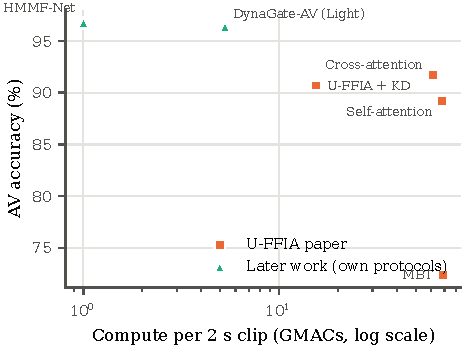
\includegraphics[width=\columnwidth]{figures/acc_vs_compute.pdf}}{\fbox{\parbox{0.9\columnwidth}{\centering run \texttt{scripts/make\_paper\_assets.py}}}}
  \caption{Accuracy versus compute (log scale) on AV-FFIA. Published models are plotted at their
  reported values and protocols; HyperAVNet uses the official split.}
  \label{fig:acc_compute}
\end{figure}

\subsection{Where to fuse: the deep-to-early study}
\label{sec:depth}
Table~\ref{tab:depth} and Fig.~\ref{fig:depth} vary the fusion set $\mathcal{S}$. Late fusion
($\mathcal{S}=\{3\}$) gives \resLateAcc\,\%; progressive fusion from stage~1 gives \resProgAcc\,\%;
the best setting is $\mathcal{S}=\resBestDepth$. Fusion is nearly free in compute: each additional HCF
stage costs about 0.17\,M parameters and under 0.02\,GMACs. Disabling the cross-modal feedback of
Eq.~\eqref{eq:feedback} at $\mathcal{S}=\{1,2,3\}$ gives \resNoFeedbackAcc\,\%.
\todo{Interpret: does accuracy grow as fusion moves earlier, saturate, or peak at mid-level stages
(an inverted U)? Does feedback help, and does the gain concentrate on Weak and Medium? Use the
single-stage rows to locate the most useful depth.}

\begin{table}[t]
  \centering
  \caption{Fusion depth (deep to early) and cross-modal feedback. Mean $\pm$ std, official split.}
  \label{tab:depth}
  \footnotesize
  \setlength{\tabcolsep}{3pt}
  \resizebox{\columnwidth}{!}{\input{tables/ablation_depth.tex}}
\end{table}

\begin{figure}[t]
  \centering
  \IfFileExists{figures/fusion_depth.pdf}{\includegraphics[width=\columnwidth]{figures/fusion_depth.pdf}}{\fbox{\parbox{0.9\columnwidth}{\centering pending runs \texttt{A\_fs*}}}}
  \caption{Accuracy as fusion moves from the last stage to all stages, with and without feedback.}
  \label{fig:depth}
\end{figure}

\subsection{Effect of the hypercomplex algebra}
\label{sec:algebra}
Table~\ref{tab:algebra} and Fig.~\ref{fig:algebra} replace every hypercomplex layer of the network with
algebra $\mathbb{A}_n$. All variants share the architecture and compute and differ only in weight
sharing. The real network ($n=1$, 7.88\,M parameters) reaches \resRealAcc\,\%, the quaternion network
(2.14\,M) \resQuatAcc\,\% and the octonion network (1.24\,M) \resOctAcc\,\%.
\todo{Interpret: if accuracy is maintained or improved down to $n=4$ or $n=8$, the Hamilton
weight sharing acts as a useful structural prior on a dataset of this size; report where accuracy
starts to drop.}

\begin{table}[t]
  \centering
  \caption{Algebra of the whole network. Compute is identical for all $n$.}
  \label{tab:algebra}
  \footnotesize
  \resizebox{\columnwidth}{!}{\input{tables/ablation_algebra.tex}}
\end{table}

\begin{figure}[t]
  \centering
  \IfFileExists{figures/algebra.pdf}{\includegraphics[width=\columnwidth]{figures/algebra.pdf}}{\fbox{\parbox{0.9\columnwidth}{\centering pending runs \texttt{B\_n*}}}}
  \caption{Accuracy against parameter count for real, complex, quaternion, octonion and sedenion networks.}
  \label{fig:algebra}
\end{figure}

\subsection{Fusion operator, regularisers and front-end}
\label{sec:operators}
Table~\ref{tab:ops} compares HCF with a hypercomplex attention bottleneck (MBT) at equal parameters,
and with gated concatenation. HCF with quaternion components gives \resHCFAcc\,\% and MBT
\resMBTAcc\,\%. In~\cite{cui2024uffia}, MBT also trailed cross-attention by a wide margin
(72.4\% vs.\ 91.7\%), which the authors attributed to attending to the modalities one after the other.
\todo{State whether parallel reading plus Hamilton mixing closes this gap, and whether octonion
components (four extra interaction terms, same parameters) help.}
The lower block of Table~\ref{tab:ops} isolates modality dropout, the auxiliary heads and the SimPF
front-end~\cite{liu2023simpf}.

\begin{table}[t]
  \centering
  \caption{Fusion operator (top), regularisers (middle) and audio front-end (bottom).}
  \label{tab:ops}
  \footnotesize
  \setlength{\tabcolsep}{3pt}
  \resizebox{\columnwidth}{!}{\input{tables/ablation_fusion_reg.tex}}
\end{table}

\subsection{Which teacher? Teacher ablation}
\label{sec:teachers}
Table~\ref{tab:teachers} reports each teacher's audio-visual and unimodal accuracy, and the accuracy
of the student distilled from it; $\Delta$ is student minus teacher. Fig.~\ref{fig:teachers} plots
student against teacher accuracy. Distillation from the default teacher (CNN10 + S3D,
\resTeacherAcc\,\%) changes the student's accuracy by \resKDGain\ points over the same student trained
without a teacher (\resNoKDAcc\,\%).
\todo{Interpret: does a stronger teacher yield a stronger student, or does the compact HMKD pair (T10,
about 1\,GMAC) distil as well as the larger teachers? Do the transformer teachers (T6, T8, T9) under-perform
on AV-FFIA, as AST and ViViT did in~\cite{cui2024uffia}?}

\begin{table*}[t]
  \centering
  \caption{Teacher ablation. Teacher params (M) and GMACs include the HCF fusion network. Student:
  HyperAVNet-Q distilled from that teacher. $\Delta$ = student $-$ teacher accuracy.}
  \label{tab:teachers}
  \small
  \resizebox{\textwidth}{!}{\input{tables/teachers.tex}}
\end{table*}

\begin{figure}[t]
  \centering
  \IfFileExists{figures/teacher_student.pdf}{\includegraphics[width=\columnwidth]{figures/teacher_student.pdf}}{\fbox{\parbox{0.9\columnwidth}{\centering pending teacher runs}}}
  \caption{Teacher accuracy against the accuracy of the student distilled from it (dashed: no distillation).}
  \label{fig:teachers}
\end{figure}

\subsection{Robustness to noise and missing modalities}
\label{sec:robustness}
Table~\ref{tab:robust} and Fig.~\ref{fig:robust} follow the robustness protocol of~\cite{cui2024uffia}.
\todo{Compare the degradation at $-10$\,dB with U-FFIA (90.7\%$\to$72.6\%) and cross-attention
(91.7\%$\to$72.7\%), only if the same bubble and pump noise was used; otherwise describe the results
as indicative. Discuss the missing-modality columns: the auxiliary heads and masked training should
keep useful accuracy when one modality is absent.}

\begin{table*}[t]
  \centering
  \caption{Robustness. Audio noise at the given SNR (U-FFIA protocol); Dark: video intensities
  $\times0.25$; Noise: Gaussian video noise, $\sigma^{2}=0.2$; $-$A / $-$V: audio / video absent.
  Published rows from~\cite{cui2024uffia} (bubble and pump noise).}
  \label{tab:robust}
  \small
  \resizebox{\textwidth}{!}{\input{tables/robustness.tex}}
\end{table*}

\begin{figure}[t]
  \centering
  \IfFileExists{figures/robustness_snr.pdf}{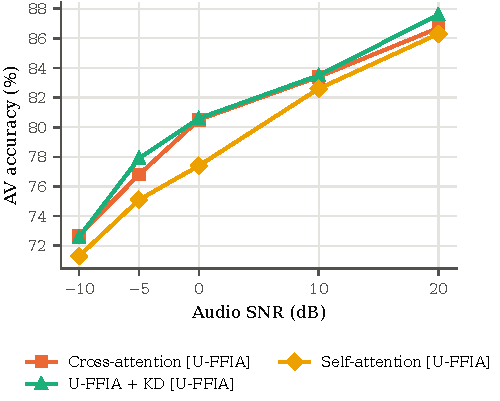
\includegraphics[width=\columnwidth]{figures/robustness_snr.pdf}}{\fbox{\parbox{0.9\columnwidth}{\centering run \texttt{scripts/make\_paper\_assets.py}}}}
  \caption{Audio-visual accuracy as the audio SNR decreases.}
  \label{fig:robust}
\end{figure}

\subsection{Evaluation protocol and data leakage}
\label{sec:protocols}
Table~\ref{tab:protocols} evaluates the same model under the three protocols of Sec.~\ref{sec:setup}:
\resOfficialAcc\,\% on the official split, \resKfoldAcc\,\% under 5-fold CV, and \resGroupedAcc\,\% on
the session-disjoint split.
\todo{If the session-disjoint accuracy is markedly lower, state that clip-level random splits
overestimate generalisation on AV-FFIA, and that published results above 95\% should be read with this
in mind.}

\begin{table}[t]
  \centering
  \caption{One model under three evaluation protocols.}
  \label{tab:protocols}
  \footnotesize
  \resizebox{\columnwidth}{!}{\input{tables/protocols.tex}}
\end{table}

\subsection{Per-class analysis}
\label{sec:perclass}
Table~\ref{tab:perclass} and Fig.~\ref{fig:confusion} give the per-class F1 and the confusion matrix
of HyperAVNet-Q (KD).
\todo{Discuss the dominant confusions, expected between the adjacent intensities Weak and Medium,
and how much the audio stream contributes to separating them.}

\begin{table}[t]
  \centering
  \caption{Per-class F1 of HyperAVNet-Q (KD), official split.}
  \label{tab:perclass}
  \footnotesize
  \input{tables/per_class.tex}
\end{table}

\begin{figure}[t]
  \centering
  \IfFileExists{figures/confusion.pdf}{\includegraphics[width=0.7\columnwidth]{figures/confusion.pdf}}{\fbox{\parbox{0.9\columnwidth}{\centering pending runs}}}
  \caption{Row-normalised confusion matrix (\%) of HyperAVNet-Q (KD), summed over seeds.}
  \label{fig:confusion}
\end{figure}

\subsection{Deployment}
\label{sec:deploy}
Table~\ref{tab:deploy} measures the cost of the two forms of the model on \resDeployDevice{} (batch 1).
In training form, every hypercomplex kernel is assembled from its $n$ blocks at each forward pass.
After reparameterisation (Sec.~\ref{sec:hyper}) the kernels are dense, and latency falls from
\resLatTrain\,ms to \resLatDeploy\,ms. The trade-off is explicit: the hypercomplex form stores and
transmits $n\times$ fewer parameters (2.14\,M), while the deployed dense form holds 7.88\,M parameters
in memory and runs faster. A device can therefore receive the compact model and expand it once at load
time.

\begin{table}[t]
  \centering
  \caption{Training-form versus reparameterised (deployed) model. Stored: parameters kept on disk and
  transmitted; Dense: parameters in memory after reparameterisation.}
  \label{tab:deploy}
  \footnotesize
  \IfFileExists{tables/deploy.tex}{\resizebox{\columnwidth}{!}{\input{tables/deploy.tex}}}{\fbox{run \texttt{profile\_model.py --out}}}
\end{table}

\subsection{Limitations}
\label{sec:limitations}
Hypercomplex layers reduce stored parameters but not arithmetic, so the compute savings come from the
compact backbone design rather than from the algebra. AV-FFIA covers one species and one tank, and
generalisation to farm conditions (turbidity, foam, other species) remains to be shown. Finally, the
discrepancies in the public data release, and the variety of protocols in the literature, limit how
precisely results can be compared across papers.

%  Numbers come from tables/*.tex and tables/macros.tex, generated by
%  scripts/make_paper_assets.py from the run folders. Re-run it after new runs.
%  Sentences marked \todo{} state a claim that must be checked against the
%  final numbers (keep, reverse or delete).
% ============================================================================
\section{Results}
\label{sec:results}

\subsection{Comparison with the state of the art}
\label{sec:main}
Table~\ref{tab:main} lists the published results on AV-FFIA with their protocols, followed by our models
under the official split. The distilled quaternion model, HyperAVNet-Q (KD), reaches
\resOurAcc\,\% accuracy (macro-F1 \resOurFone\,\%) with \resOurParams\,M parameters and
\resOurGMACs\,GMACs per clip. That is 10.1$\times$ fewer parameters and 13.1$\times$ fewer MACs than
U-FFIA~\cite{cui2024uffia}, and 16.4$\times$ / 51.6$\times$ fewer than the cross-attention model.
\todo{Position against the strongest comparable result: DynaGate-AV reports 96.4--96.5\% on the same
official split rule, and HMMF-Net 96.77\% under 5-fold CV (Table~\ref{tab:protocols}). State whether
HyperAVNet exceeds, matches or trails them; LDMF and HMKD use filtered subsets and are not comparable.}
Fig.~\ref{fig:acc_compute} places all models on an accuracy--compute plane.
Its single-modality heads reach \resOurAccA\,\% (audio) and \resOurAccV\,\% (video), against the
best published single-modality models, Pre-CNN10 (85.9\%) and Pretrained-S3D (89.8\%)~\cite{cui2024uffia}.

\begin{table*}[t]
  \centering
  \caption{Comparison on AV-FFIA. Compute is in GMACs per 2\,s clip; U-FFIA's ``FLOPs'' are MACs.
  Published numbers are quoted with their own protocol and are not directly comparable across
  protocols. $^\dagger$Not verified against the full paper (taken from secondary sources). Our
  rows: official split, mean $\pm$ std over three seeds.}
  \label{tab:main}
  \small
  \resizebox{\textwidth}{!}{\begin{tabular}{llrrrrl}
\toprule
Method & Mod. & Params (M) & GMACs & Acc. (\%) & F1 (\%) & Protocol \\
\midrule
Pre-CNN10~\cite{cui2024uffia} & A & 5.00 & 3.347 & 85.9 & -- & paper split \\
Pretrained-S3D~\cite{cui2024uffia} & V & 7.90 & 22.826 & 89.8 & -- & paper split \\
Self-attention~\cite{cui2024uffia} & AV & 47.70 & 68.404 & 89.2 & -- & paper split \\
MBT~\cite{cui2024uffia} & AV & 47.69 & 68.690 & 72.4 & -- & paper split \\
Cross-attention~\cite{cui2024uffia} & AV & 35.08 & 60.933 & 91.7 & -- & paper split \\
U-FFIA + KD~\cite{cui2024uffia} & AV & 21.63 & 15.488 & 90.7 & -- & paper split \\
\midrule
ACAF-Net~\cite{acafnet2025}$^\dagger$ & AV & -- & -- & 95.4 & -- & random split \\
DynaGate-AV (Light)~\cite{dynagate2026} & AV & -- & 5.290 & 96.4 & -- & official split, 19,963 clips \\
HMMF-Net~\cite{hmmfnet2026}$^\dagger$ & AV & 3.99 & 1.002 & 96.8 & 96.9 & 5-fold CV \\
HMKD~\cite{hmkd2026}$^\dagger$ & AV & -- & -- & 97.5 & -- & 26,843-pair holdout \\
LDMF~\cite{ldmf2026}$^\dagger$ & AV & 7.10 & -- & 98.2 & -- & filtered subset \\
\midrule
Real late-concat baseline (ours, re-run) & AV & -- & -- & -- & -- & official split \\
Teacher: CNN10 + S3D + HCF & AV & -- & -- & -- & -- & official split \\
Teacher: EfficientAT + MoViNet-A0 + HCF & AV & -- & -- & -- & -- & official split \\
HyperAVNet-Q (no KD) & AV & -- & -- & -- & -- & official split \\
\textbf{HyperAVNet-Q (KD)} & AV & -- & -- & -- & -- & official split \\
HyperAVNet-P (pretrained, no KD) & AV & -- & -- & -- & -- & official split \\
HyperAVNet-P (pretrained, KD) & AV & -- & -- & -- & -- & official split \\
HyperAVNet-O (KD) & AV & -- & -- & -- & -- & official split \\
\bottomrule
\end{tabular}
}
\end{table*}

\begin{figure}[t]
  \centering
  \IfFileExists{figures/acc_vs_compute.pdf}{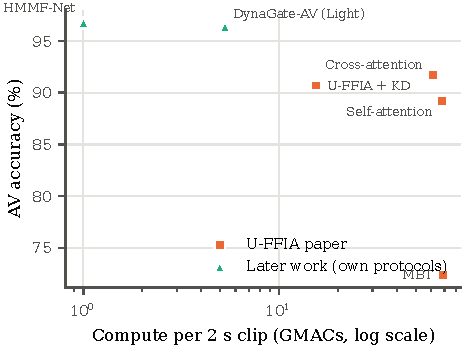
\includegraphics[width=\columnwidth]{figures/acc_vs_compute.pdf}}{\fbox{\parbox{0.9\columnwidth}{\centering run \texttt{scripts/make\_paper\_assets.py}}}}
  \caption{Accuracy versus compute (log scale) on AV-FFIA. Published models are plotted at their
  reported values and protocols; HyperAVNet uses the official split.}
  \label{fig:acc_compute}
\end{figure}

\subsection{Where to fuse: the deep-to-early study}
\label{sec:depth}
Table~\ref{tab:depth} and Fig.~\ref{fig:depth} vary the fusion set $\mathcal{S}$. Late fusion
($\mathcal{S}=\{3\}$) gives \resLateAcc\,\%; progressive fusion from stage~1 gives \resProgAcc\,\%;
the best setting is $\mathcal{S}=\resBestDepth$. Fusion is nearly free in compute: each additional HCF
stage costs about 0.17\,M parameters and under 0.02\,GMACs. Disabling the cross-modal feedback of
Eq.~\eqref{eq:feedback} at $\mathcal{S}=\{1,2,3\}$ gives \resNoFeedbackAcc\,\%.
\todo{Interpret: does accuracy grow as fusion moves earlier, saturate, or peak at mid-level stages
(an inverted U)? Does feedback help, and does the gain concentrate on Weak and Medium? Use the
single-stage rows to locate the most useful depth.}

\begin{table}[t]
  \centering
  \caption{Fusion depth (deep to early) and cross-modal feedback. Mean $\pm$ std, official split.}
  \label{tab:depth}
  \footnotesize
  \setlength{\tabcolsep}{3pt}
  \resizebox{\columnwidth}{!}{\begin{tabular}{lrrrrrr}
\toprule
Fusion stages $\mathcal{S}$ & Params (M) & GMACs & Acc. & F1 & A-only & V-only \\
\midrule
$\{3\}$ (late) & -- & -- & -- & -- & -- & -- \\
$\{2,3\}$ & -- & -- & -- & -- & -- & -- \\
$\{1,2,3\}$ & -- & -- & -- & -- & -- & -- \\
$\{0,1,2,3\}$ & -- & -- & -- & -- & -- & -- \\
\midrule
$\{0\}$ & -- & -- & -- & -- & -- & -- \\
$\{1\}$ & -- & -- & -- & -- & -- & -- \\
$\{2\}$ & -- & -- & -- & -- & -- & -- \\
\midrule
$\{1,2,3\}$ w/o feedback & -- & -- & -- & -- & -- & -- \\
\bottomrule
\end{tabular}
}
\end{table}

\begin{figure}[t]
  \centering
  \IfFileExists{figures/fusion_depth.pdf}{\includegraphics[width=\columnwidth]{figures/fusion_depth.pdf}}{\fbox{\parbox{0.9\columnwidth}{\centering pending runs \texttt{A\_fs*}}}}
  \caption{Accuracy as fusion moves from the last stage to all stages, with and without feedback.}
  \label{fig:depth}
\end{figure}

\subsection{Effect of the hypercomplex algebra}
\label{sec:algebra}
Table~\ref{tab:algebra} and Fig.~\ref{fig:algebra} replace every hypercomplex layer of the network with
algebra $\mathbb{A}_n$. All variants share the architecture and compute and differ only in weight
sharing. The real network ($n=1$, 7.88\,M parameters) reaches \resRealAcc\,\%, the quaternion network
(2.14\,M) \resQuatAcc\,\% and the octonion network (1.24\,M) \resOctAcc\,\%.
\todo{Interpret: if accuracy is maintained or improved down to $n=4$ or $n=8$, the Hamilton
weight sharing acts as a useful structural prior on a dataset of this size; report where accuracy
starts to drop.}

\begin{table}[t]
  \centering
  \caption{Algebra of the whole network. Compute is identical for all $n$.}
  \label{tab:algebra}
  \footnotesize
  \resizebox{\columnwidth}{!}{\begin{tabular}{lrrrr}
\toprule
Algebra & Params (M) & GMACs & Acc. & F1 \\
\midrule
Real ($n{=}1$) & -- & -- & -- & -- \\
Complex ($n{=}2$) & -- & -- & -- & -- \\
Quaternion ($n{=}4$) & -- & -- & -- & -- \\
Octonion ($n{=}8$) & -- & -- & -- & -- \\
Sedenion ($n{=}16$) & -- & -- & -- & -- \\
\bottomrule
\end{tabular}
}
\end{table}

\begin{figure}[t]
  \centering
  \IfFileExists{figures/algebra.pdf}{\includegraphics[width=\columnwidth]{figures/algebra.pdf}}{\fbox{\parbox{0.9\columnwidth}{\centering pending runs \texttt{B\_n*}}}}
  \caption{Accuracy against parameter count for real, complex, quaternion, octonion and sedenion networks.}
  \label{fig:algebra}
\end{figure}

\subsection{Fusion operator, regularisers and front-end}
\label{sec:operators}
Table~\ref{tab:ops} compares HCF with a hypercomplex attention bottleneck (MBT) at equal parameters,
and with gated concatenation. HCF with quaternion components gives \resHCFAcc\,\% and MBT
\resMBTAcc\,\%. In~\cite{cui2024uffia}, MBT also trailed cross-attention by a wide margin
(72.4\% vs.\ 91.7\%), which the authors attributed to attending to the modalities one after the other.
\todo{State whether parallel reading plus Hamilton mixing closes this gap, and whether octonion
components (four extra interaction terms, same parameters) help.}
The lower block of Table~\ref{tab:ops} isolates modality dropout, the auxiliary heads and the SimPF
front-end~\cite{liu2023simpf}.

\begin{table}[t]
  \centering
  \caption{Fusion operator (top), regularisers (middle) and audio front-end (bottom).}
  \label{tab:ops}
  \footnotesize
  \setlength{\tabcolsep}{3pt}
  \resizebox{\columnwidth}{!}{\begin{tabular}{lrrrrr}
\toprule
Variant & Params (M) & Acc. & F1 & A-only & V-only \\
\midrule
HCF, complex components & -- & -- & -- & -- & -- \\
HCF, quaternion components & -- & -- & -- & -- & -- \\
HCF, octonion components & -- & -- & -- & -- & -- \\
Hypercomplex MBT & -- & -- & -- & -- & -- \\
Gated concatenation & -- & -- & -- & -- & -- \\
\midrule
w/o modality dropout ($p{=}0$) & -- & -- & -- & -- & -- \\
modality dropout $p{=}0.25$ & -- & -- & -- & -- & -- \\
w/o auxiliary heads & -- & -- & -- & -- & -- \\
\midrule
SimPF front-end ($k{=}0.5$) & -- & -- & -- & -- & -- \\
\bottomrule
\end{tabular}
}
\end{table}

\subsection{Which teacher? Teacher ablation}
\label{sec:teachers}
Table~\ref{tab:teachers} reports each teacher's audio-visual and unimodal accuracy, and the accuracy
of the student distilled from it; $\Delta$ is student minus teacher. Fig.~\ref{fig:teachers} plots
student against teacher accuracy. Distillation from the default teacher (CNN10 + S3D,
\resTeacherAcc\,\%) changes the student's accuracy by \resKDGain\ points over the same student trained
without a teacher (\resNoKDAcc\,\%).
\todo{Interpret: does a stronger teacher yield a stronger student, or does the compact HMKD pair (T10,
about 1\,GMAC) distil as well as the larger teachers? Do the transformer teachers (T6, T8, T9) under-perform
on AV-FFIA, as AST and ViViT did in~\cite{cui2024uffia}?}

\begin{table*}[t]
  \centering
  \caption{Teacher ablation. Teacher params (M) and GMACs include the HCF fusion network. Student:
  HyperAVNet-Q distilled from that teacher. $\Delta$ = student $-$ teacher accuracy.}
  \label{tab:teachers}
  \small
  \resizebox{\textwidth}{!}{\begin{tabular}{llrrrrrrr}
\toprule
ID & Audio / video teacher & Params & GMACs & Teacher AV & A-only & V-only & Student & $\Delta$ \\
\midrule
T1 & CNN10 / S3D & -- & -- & -- & -- & -- & -- & -- \\
T2 & CNN14 / S3D & -- & -- & -- & -- & -- & -- & -- \\
T3 & CNN10 / R(2+1)D-18 & -- & -- & -- & -- & -- & -- & -- \\
T4 & CNN10 / ConvNeXt-T (frames) & -- & -- & -- & -- & -- & -- & -- \\
T5 & EffNet-B0 (mel) / S3D & -- & -- & -- & -- & -- & -- & -- \\
T6 & AST / VideoMAE-B & -- & -- & -- & -- & -- & -- & -- \\
T7 & CNN10 / X3D-M & -- & -- & -- & -- & -- & -- & -- \\
T8 & AST / S3D & -- & -- & -- & -- & -- & -- & -- \\
T9 & CNN10 / VideoMAE-B & -- & -- & -- & -- & -- & -- & -- \\
T10 & EfficientAT / MoViNet-A0 & -- & -- & -- & -- & -- & -- & -- \\
\midrule
-- & no teacher (no KD) & -- & -- & -- & -- & -- & -- & -- \\
\bottomrule
\end{tabular}
}
\end{table*}

\begin{figure}[t]
  \centering
  \IfFileExists{figures/teacher_student.pdf}{\includegraphics[width=\columnwidth]{figures/teacher_student.pdf}}{\fbox{\parbox{0.9\columnwidth}{\centering pending teacher runs}}}
  \caption{Teacher accuracy against the accuracy of the student distilled from it (dashed: no distillation).}
  \label{fig:teachers}
\end{figure}

\subsection{Robustness to noise and missing modalities}
\label{sec:robustness}
Table~\ref{tab:robust} and Fig.~\ref{fig:robust} follow the robustness protocol of~\cite{cui2024uffia}.
\todo{Compare the degradation at $-10$\,dB with U-FFIA (90.7\%$\to$72.6\%) and cross-attention
(91.7\%$\to$72.7\%), only if the same bubble and pump noise was used; otherwise describe the results
as indicative. Discuss the missing-modality columns: the auxiliary heads and masked training should
keep useful accuracy when one modality is absent.}

\begin{table*}[t]
  \centering
  \caption{Robustness. Audio noise at the given SNR (U-FFIA protocol); Dark: video intensities
  $\times0.25$; Noise: Gaussian video noise, $\sigma^{2}=0.2$; $-$A / $-$V: audio / video absent.
  Published rows from~\cite{cui2024uffia} (bubble and pump noise).}
  \label{tab:robust}
  \small
  \resizebox{\textwidth}{!}{\begin{tabular}{lrrrrrrrrrr}
\toprule
Method & Clean & -10\,dB & -5\,dB & +0\,dB & +10\,dB & +20\,dB & Dark & Noise & $-$A & $-$V \\
\midrule
Cross-attention~\cite{cui2024uffia} & 91.7 & 72.7 & 76.8 & 80.5 & 83.4 & 86.7 & -- & -- & -- & -- \\
U-FFIA + KD~\cite{cui2024uffia} & 90.7 & 72.6 & 77.9 & 80.6 & 83.5 & 87.6 & -- & -- & -- & -- \\
Self-attention~\cite{cui2024uffia} & 89.2 & 71.3 & 75.1 & 77.4 & 82.6 & 86.3 & -- & -- & -- & -- \\
\midrule
Teacher (CNN10 + S3D) & -- & -- & -- & -- & -- & -- & -- & -- & -- & -- \\
\textbf{HyperAVNet-Q (KD)} & -- & -- & -- & -- & -- & -- & -- & -- & -- & -- \\
\bottomrule
\end{tabular}
}
\end{table*}

\begin{figure}[t]
  \centering
  \IfFileExists{figures/robustness_snr.pdf}{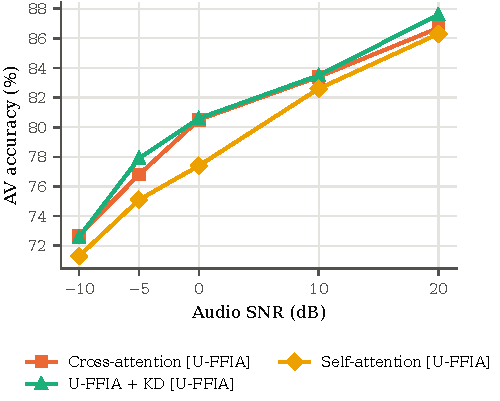
\includegraphics[width=\columnwidth]{figures/robustness_snr.pdf}}{\fbox{\parbox{0.9\columnwidth}{\centering run \texttt{scripts/make\_paper\_assets.py}}}}
  \caption{Audio-visual accuracy as the audio SNR decreases.}
  \label{fig:robust}
\end{figure}

\subsection{Evaluation protocol and data leakage}
\label{sec:protocols}
Table~\ref{tab:protocols} evaluates the same model under the three protocols of Sec.~\ref{sec:setup}:
\resOfficialAcc\,\% on the official split, \resKfoldAcc\,\% under 5-fold CV, and \resGroupedAcc\,\% on
the session-disjoint split.
\todo{If the session-disjoint accuracy is markedly lower, state that clip-level random splits
overestimate generalisation on AV-FFIA, and that published results above 95\% should be read with this
in mind.}

\begin{table}[t]
  \centering
  \caption{One model under three evaluation protocols.}
  \label{tab:protocols}
  \footnotesize
  \resizebox{\columnwidth}{!}{\begin{tabular}{lrrr}
\toprule
Evaluation protocol & Runs & Acc. & F1 \\
\midrule
Official code split (700/700 per class) & -- & -- & -- \\
5-fold stratified CV & -- & -- & -- \\
Session-disjoint (whole recording dates) & -- & -- & -- \\
\bottomrule
\end{tabular}
}
\end{table}

\subsection{Per-class analysis}
\label{sec:perclass}
Table~\ref{tab:perclass} and Fig.~\ref{fig:confusion} give the per-class F1 and the confusion matrix
of HyperAVNet-Q (KD).
\todo{Discuss the dominant confusions, expected between the adjacent intensities Weak and Medium,
and how much the audio stream contributes to separating them.}

\begin{table}[t]
  \centering
  \caption{Per-class F1 of HyperAVNet-Q (KD), official split.}
  \label{tab:perclass}
  \footnotesize
  \begin{tabular}{lr}
\toprule
Class & F1 (\%) \\
\midrule
None & -- \\
Strong & -- \\
Medium & -- \\
Weak & -- \\
\bottomrule
\end{tabular}

\end{table}

\begin{figure}[t]
  \centering
  \IfFileExists{figures/confusion.pdf}{\includegraphics[width=0.7\columnwidth]{figures/confusion.pdf}}{\fbox{\parbox{0.9\columnwidth}{\centering pending runs}}}
  \caption{Row-normalised confusion matrix (\%) of HyperAVNet-Q (KD), summed over seeds.}
  \label{fig:confusion}
\end{figure}

\subsection{Deployment}
\label{sec:deploy}
Table~\ref{tab:deploy} measures the cost of the two forms of the model on \resDeployDevice{} (batch 1).
In training form, every hypercomplex kernel is assembled from its $n$ blocks at each forward pass.
After reparameterisation (Sec.~\ref{sec:hyper}) the kernels are dense, and latency falls from
\resLatTrain\,ms to \resLatDeploy\,ms. The trade-off is explicit: the hypercomplex form stores and
transmits $n\times$ fewer parameters (2.14\,M), while the deployed dense form holds 7.88\,M parameters
in memory and runs faster. A device can therefore receive the compact model and expand it once at load
time.

\begin{table}[t]
  \centering
  \caption{Training-form versus reparameterised (deployed) model. Stored: parameters kept on disk and
  transmitted; Dense: parameters in memory after reparameterisation.}
  \label{tab:deploy}
  \footnotesize
  \IfFileExists{tables/deploy.tex}{\resizebox{\columnwidth}{!}{\begin{tabular}{lrrrrrr}
\toprule
Model & Stored (M) & Dense (M) & GMACs & Train-form (ms) & Deployed (ms) & Speed-up \\
\midrule
-- & -- & -- & -- & -- & -- & -- \\
\bottomrule
\end{tabular}
}}{\fbox{run \texttt{profile\_model.py --out}}}
\end{table}

\subsection{Limitations}
\label{sec:limitations}
Hypercomplex layers reduce stored parameters but not arithmetic, so the compute savings come from the
compact backbone design rather than from the algebra. AV-FFIA covers one species and one tank, and
generalisation to farm conditions (turbidity, foam, other species) remains to be shown. Finally, the
discrepancies in the public data release, and the variety of protocols in the literature, limit how
precisely results can be compared across papers.

%  Numbers come from tables/*.tex and tables/macros.tex, generated by
%  scripts/make_paper_assets.py from the run folders. Re-run it after new runs.
%  Sentences marked \todo{} state a claim that must be checked against the
%  final numbers (keep, reverse or delete).
% ============================================================================
\section{Results}
\label{sec:results}

\subsection{Comparison with the state of the art}
\label{sec:main}
Table~\ref{tab:main} lists the published results on AV-FFIA with their protocols, followed by our models
under the official split. The distilled quaternion model, HyperAVNet-Q (KD), reaches
\resOurAcc\,\% accuracy (macro-F1 \resOurFone\,\%) with \resOurParams\,M parameters and
\resOurGMACs\,GMACs per clip. That is 10.1$\times$ fewer parameters and 13.1$\times$ fewer MACs than
U-FFIA~\cite{cui2024uffia}, and 16.4$\times$ / 51.6$\times$ fewer than the cross-attention model.
\todo{Position against the strongest comparable result: DynaGate-AV reports 96.4--96.5\% on the same
official split rule, and HMMF-Net 96.77\% under 5-fold CV (Table~\ref{tab:protocols}). State whether
HyperAVNet exceeds, matches or trails them; LDMF and HMKD use filtered subsets and are not comparable.}
Fig.~\ref{fig:acc_compute} places all models on an accuracy--compute plane.
Its single-modality heads reach \resOurAccA\,\% (audio) and \resOurAccV\,\% (video), against the
best published single-modality models, Pre-CNN10 (85.9\%) and Pretrained-S3D (89.8\%)~\cite{cui2024uffia}.

\begin{table*}[t]
  \centering
  \caption{Comparison on AV-FFIA. Compute is in GMACs per 2\,s clip; U-FFIA's ``FLOPs'' are MACs.
  Published numbers are quoted with their own protocol and are not directly comparable across
  protocols. $^\dagger$Not verified against the full paper (taken from secondary sources). Our
  rows: official split, mean $\pm$ std over three seeds.}
  \label{tab:main}
  \small
  \resizebox{\textwidth}{!}{\begin{tabular}{llrrrrl}
\toprule
Method & Mod. & Params (M) & GMACs & Acc. (\%) & F1 (\%) & Protocol \\
\midrule
Pre-CNN10~\cite{cui2024uffia} & A & 5.00 & 3.347 & 85.9 & -- & paper split \\
Pretrained-S3D~\cite{cui2024uffia} & V & 7.90 & 22.826 & 89.8 & -- & paper split \\
Self-attention~\cite{cui2024uffia} & AV & 47.70 & 68.404 & 89.2 & -- & paper split \\
MBT~\cite{cui2024uffia} & AV & 47.69 & 68.690 & 72.4 & -- & paper split \\
Cross-attention~\cite{cui2024uffia} & AV & 35.08 & 60.933 & 91.7 & -- & paper split \\
U-FFIA + KD~\cite{cui2024uffia} & AV & 21.63 & 15.488 & 90.7 & -- & paper split \\
\midrule
ACAF-Net~\cite{acafnet2025}$^\dagger$ & AV & -- & -- & 95.4 & -- & random split \\
DynaGate-AV (Light)~\cite{dynagate2026} & AV & -- & 5.290 & 96.4 & -- & official split, 19,963 clips \\
HMMF-Net~\cite{hmmfnet2026}$^\dagger$ & AV & 3.99 & 1.002 & 96.8 & 96.9 & 5-fold CV \\
HMKD~\cite{hmkd2026}$^\dagger$ & AV & -- & -- & 97.5 & -- & 26,843-pair holdout \\
LDMF~\cite{ldmf2026}$^\dagger$ & AV & 7.10 & -- & 98.2 & -- & filtered subset \\
\midrule
Real late-concat baseline (ours, re-run) & AV & -- & -- & -- & -- & official split \\
Teacher: CNN10 + S3D + HCF & AV & -- & -- & -- & -- & official split \\
Teacher: EfficientAT + MoViNet-A0 + HCF & AV & -- & -- & -- & -- & official split \\
HyperAVNet-Q (no KD) & AV & -- & -- & -- & -- & official split \\
\textbf{HyperAVNet-Q (KD)} & AV & -- & -- & -- & -- & official split \\
HyperAVNet-P (pretrained, no KD) & AV & -- & -- & -- & -- & official split \\
HyperAVNet-P (pretrained, KD) & AV & -- & -- & -- & -- & official split \\
HyperAVNet-O (KD) & AV & -- & -- & -- & -- & official split \\
\bottomrule
\end{tabular}
}
\end{table*}

\begin{figure}[t]
  \centering
  \IfFileExists{figures/acc_vs_compute.pdf}{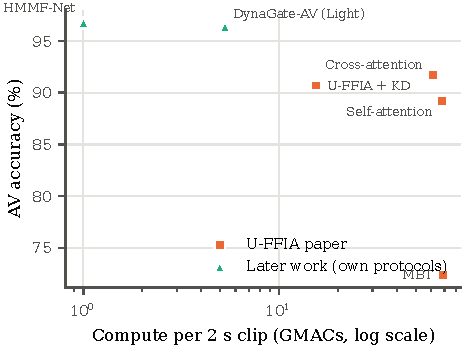
\includegraphics[width=\columnwidth]{figures/acc_vs_compute.pdf}}{\fbox{\parbox{0.9\columnwidth}{\centering run \texttt{scripts/make\_paper\_assets.py}}}}
  \caption{Accuracy versus compute (log scale) on AV-FFIA. Published models are plotted at their
  reported values and protocols; HyperAVNet uses the official split.}
  \label{fig:acc_compute}
\end{figure}

\subsection{Where to fuse: the deep-to-early study}
\label{sec:depth}
Table~\ref{tab:depth} and Fig.~\ref{fig:depth} vary the fusion set $\mathcal{S}$. Late fusion
($\mathcal{S}=\{3\}$) gives \resLateAcc\,\%; progressive fusion from stage~1 gives \resProgAcc\,\%;
the best setting is $\mathcal{S}=\resBestDepth$. Fusion is nearly free in compute: each additional HCF
stage costs about 0.17\,M parameters and under 0.02\,GMACs. Disabling the cross-modal feedback of
Eq.~\eqref{eq:feedback} at $\mathcal{S}=\{1,2,3\}$ gives \resNoFeedbackAcc\,\%.
\todo{Interpret: does accuracy grow as fusion moves earlier, saturate, or peak at mid-level stages
(an inverted U)? Does feedback help, and does the gain concentrate on Weak and Medium? Use the
single-stage rows to locate the most useful depth.}

\begin{table}[t]
  \centering
  \caption{Fusion depth (deep to early) and cross-modal feedback. Mean $\pm$ std, official split.}
  \label{tab:depth}
  \footnotesize
  \setlength{\tabcolsep}{3pt}
  \resizebox{\columnwidth}{!}{\begin{tabular}{lrrrrrr}
\toprule
Fusion stages $\mathcal{S}$ & Params (M) & GMACs & Acc. & F1 & A-only & V-only \\
\midrule
$\{3\}$ (late) & -- & -- & -- & -- & -- & -- \\
$\{2,3\}$ & -- & -- & -- & -- & -- & -- \\
$\{1,2,3\}$ & -- & -- & -- & -- & -- & -- \\
$\{0,1,2,3\}$ & -- & -- & -- & -- & -- & -- \\
\midrule
$\{0\}$ & -- & -- & -- & -- & -- & -- \\
$\{1\}$ & -- & -- & -- & -- & -- & -- \\
$\{2\}$ & -- & -- & -- & -- & -- & -- \\
\midrule
$\{1,2,3\}$ w/o feedback & -- & -- & -- & -- & -- & -- \\
\bottomrule
\end{tabular}
}
\end{table}

\begin{figure}[t]
  \centering
  \IfFileExists{figures/fusion_depth.pdf}{\includegraphics[width=\columnwidth]{figures/fusion_depth.pdf}}{\fbox{\parbox{0.9\columnwidth}{\centering pending runs \texttt{A\_fs*}}}}
  \caption{Accuracy as fusion moves from the last stage to all stages, with and without feedback.}
  \label{fig:depth}
\end{figure}

\subsection{Effect of the hypercomplex algebra}
\label{sec:algebra}
Table~\ref{tab:algebra} and Fig.~\ref{fig:algebra} replace every hypercomplex layer of the network with
algebra $\mathbb{A}_n$. All variants share the architecture and compute and differ only in weight
sharing. The real network ($n=1$, 7.88\,M parameters) reaches \resRealAcc\,\%, the quaternion network
(2.14\,M) \resQuatAcc\,\% and the octonion network (1.24\,M) \resOctAcc\,\%.
\todo{Interpret: if accuracy is maintained or improved down to $n=4$ or $n=8$, the Hamilton
weight sharing acts as a useful structural prior on a dataset of this size; report where accuracy
starts to drop.}

\begin{table}[t]
  \centering
  \caption{Algebra of the whole network. Compute is identical for all $n$.}
  \label{tab:algebra}
  \footnotesize
  \resizebox{\columnwidth}{!}{\begin{tabular}{lrrrr}
\toprule
Algebra & Params (M) & GMACs & Acc. & F1 \\
\midrule
Real ($n{=}1$) & -- & -- & -- & -- \\
Complex ($n{=}2$) & -- & -- & -- & -- \\
Quaternion ($n{=}4$) & -- & -- & -- & -- \\
Octonion ($n{=}8$) & -- & -- & -- & -- \\
Sedenion ($n{=}16$) & -- & -- & -- & -- \\
\bottomrule
\end{tabular}
}
\end{table}

\begin{figure}[t]
  \centering
  \IfFileExists{figures/algebra.pdf}{\includegraphics[width=\columnwidth]{figures/algebra.pdf}}{\fbox{\parbox{0.9\columnwidth}{\centering pending runs \texttt{B\_n*}}}}
  \caption{Accuracy against parameter count for real, complex, quaternion, octonion and sedenion networks.}
  \label{fig:algebra}
\end{figure}

\subsection{Fusion operator, regularisers and front-end}
\label{sec:operators}
Table~\ref{tab:ops} compares HCF with a hypercomplex attention bottleneck (MBT) at equal parameters,
and with gated concatenation. HCF with quaternion components gives \resHCFAcc\,\% and MBT
\resMBTAcc\,\%. In~\cite{cui2024uffia}, MBT also trailed cross-attention by a wide margin
(72.4\% vs.\ 91.7\%), which the authors attributed to attending to the modalities one after the other.
\todo{State whether parallel reading plus Hamilton mixing closes this gap, and whether octonion
components (four extra interaction terms, same parameters) help.}
The lower block of Table~\ref{tab:ops} isolates modality dropout, the auxiliary heads and the SimPF
front-end~\cite{liu2023simpf}.

\begin{table}[t]
  \centering
  \caption{Fusion operator (top), regularisers (middle) and audio front-end (bottom).}
  \label{tab:ops}
  \footnotesize
  \setlength{\tabcolsep}{3pt}
  \resizebox{\columnwidth}{!}{\begin{tabular}{lrrrrr}
\toprule
Variant & Params (M) & Acc. & F1 & A-only & V-only \\
\midrule
HCF, complex components & -- & -- & -- & -- & -- \\
HCF, quaternion components & -- & -- & -- & -- & -- \\
HCF, octonion components & -- & -- & -- & -- & -- \\
Hypercomplex MBT & -- & -- & -- & -- & -- \\
Gated concatenation & -- & -- & -- & -- & -- \\
\midrule
w/o modality dropout ($p{=}0$) & -- & -- & -- & -- & -- \\
modality dropout $p{=}0.25$ & -- & -- & -- & -- & -- \\
w/o auxiliary heads & -- & -- & -- & -- & -- \\
\midrule
SimPF front-end ($k{=}0.5$) & -- & -- & -- & -- & -- \\
\bottomrule
\end{tabular}
}
\end{table}

\subsection{Which teacher? Teacher ablation}
\label{sec:teachers}
Table~\ref{tab:teachers} reports each teacher's audio-visual and unimodal accuracy, and the accuracy
of the student distilled from it; $\Delta$ is student minus teacher. Fig.~\ref{fig:teachers} plots
student against teacher accuracy. Distillation from the default teacher (CNN10 + S3D,
\resTeacherAcc\,\%) changes the student's accuracy by \resKDGain\ points over the same student trained
without a teacher (\resNoKDAcc\,\%).
\todo{Interpret: does a stronger teacher yield a stronger student, or does the compact HMKD pair (T10,
about 1\,GMAC) distil as well as the larger teachers? Do the transformer teachers (T6, T8, T9) under-perform
on AV-FFIA, as AST and ViViT did in~\cite{cui2024uffia}?}

\begin{table*}[t]
  \centering
  \caption{Teacher ablation. Teacher params (M) and GMACs include the HCF fusion network. Student:
  HyperAVNet-Q distilled from that teacher. $\Delta$ = student $-$ teacher accuracy.}
  \label{tab:teachers}
  \small
  \resizebox{\textwidth}{!}{\begin{tabular}{llrrrrrrr}
\toprule
ID & Audio / video teacher & Params & GMACs & Teacher AV & A-only & V-only & Student & $\Delta$ \\
\midrule
T1 & CNN10 / S3D & -- & -- & -- & -- & -- & -- & -- \\
T2 & CNN14 / S3D & -- & -- & -- & -- & -- & -- & -- \\
T3 & CNN10 / R(2+1)D-18 & -- & -- & -- & -- & -- & -- & -- \\
T4 & CNN10 / ConvNeXt-T (frames) & -- & -- & -- & -- & -- & -- & -- \\
T5 & EffNet-B0 (mel) / S3D & -- & -- & -- & -- & -- & -- & -- \\
T6 & AST / VideoMAE-B & -- & -- & -- & -- & -- & -- & -- \\
T7 & CNN10 / X3D-M & -- & -- & -- & -- & -- & -- & -- \\
T8 & AST / S3D & -- & -- & -- & -- & -- & -- & -- \\
T9 & CNN10 / VideoMAE-B & -- & -- & -- & -- & -- & -- & -- \\
T10 & EfficientAT / MoViNet-A0 & -- & -- & -- & -- & -- & -- & -- \\
\midrule
-- & no teacher (no KD) & -- & -- & -- & -- & -- & -- & -- \\
\bottomrule
\end{tabular}
}
\end{table*}

\begin{figure}[t]
  \centering
  \IfFileExists{figures/teacher_student.pdf}{\includegraphics[width=\columnwidth]{figures/teacher_student.pdf}}{\fbox{\parbox{0.9\columnwidth}{\centering pending teacher runs}}}
  \caption{Teacher accuracy against the accuracy of the student distilled from it (dashed: no distillation).}
  \label{fig:teachers}
\end{figure}

\subsection{Robustness to noise and missing modalities}
\label{sec:robustness}
Table~\ref{tab:robust} and Fig.~\ref{fig:robust} follow the robustness protocol of~\cite{cui2024uffia}.
\todo{Compare the degradation at $-10$\,dB with U-FFIA (90.7\%$\to$72.6\%) and cross-attention
(91.7\%$\to$72.7\%), only if the same bubble and pump noise was used; otherwise describe the results
as indicative. Discuss the missing-modality columns: the auxiliary heads and masked training should
keep useful accuracy when one modality is absent.}

\begin{table*}[t]
  \centering
  \caption{Robustness. Audio noise at the given SNR (U-FFIA protocol); Dark: video intensities
  $\times0.25$; Noise: Gaussian video noise, $\sigma^{2}=0.2$; $-$A / $-$V: audio / video absent.
  Published rows from~\cite{cui2024uffia} (bubble and pump noise).}
  \label{tab:robust}
  \small
  \resizebox{\textwidth}{!}{\begin{tabular}{lrrrrrrrrrr}
\toprule
Method & Clean & -10\,dB & -5\,dB & +0\,dB & +10\,dB & +20\,dB & Dark & Noise & $-$A & $-$V \\
\midrule
Cross-attention~\cite{cui2024uffia} & 91.7 & 72.7 & 76.8 & 80.5 & 83.4 & 86.7 & -- & -- & -- & -- \\
U-FFIA + KD~\cite{cui2024uffia} & 90.7 & 72.6 & 77.9 & 80.6 & 83.5 & 87.6 & -- & -- & -- & -- \\
Self-attention~\cite{cui2024uffia} & 89.2 & 71.3 & 75.1 & 77.4 & 82.6 & 86.3 & -- & -- & -- & -- \\
\midrule
Teacher (CNN10 + S3D) & -- & -- & -- & -- & -- & -- & -- & -- & -- & -- \\
\textbf{HyperAVNet-Q (KD)} & -- & -- & -- & -- & -- & -- & -- & -- & -- & -- \\
\bottomrule
\end{tabular}
}
\end{table*}

\begin{figure}[t]
  \centering
  \IfFileExists{figures/robustness_snr.pdf}{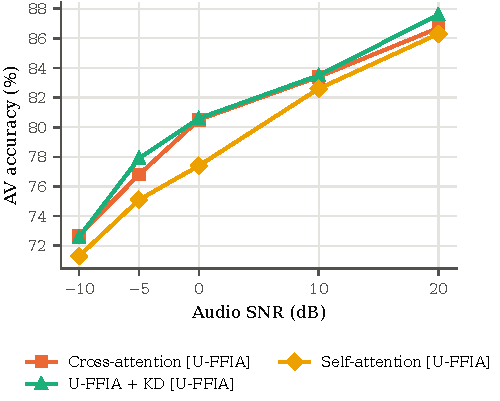
\includegraphics[width=\columnwidth]{figures/robustness_snr.pdf}}{\fbox{\parbox{0.9\columnwidth}{\centering run \texttt{scripts/make\_paper\_assets.py}}}}
  \caption{Audio-visual accuracy as the audio SNR decreases.}
  \label{fig:robust}
\end{figure}

\subsection{Evaluation protocol and data leakage}
\label{sec:protocols}
Table~\ref{tab:protocols} evaluates the same model under the three protocols of Sec.~\ref{sec:setup}:
\resOfficialAcc\,\% on the official split, \resKfoldAcc\,\% under 5-fold CV, and \resGroupedAcc\,\% on
the session-disjoint split.
\todo{If the session-disjoint accuracy is markedly lower, state that clip-level random splits
overestimate generalisation on AV-FFIA, and that published results above 95\% should be read with this
in mind.}

\begin{table}[t]
  \centering
  \caption{One model under three evaluation protocols.}
  \label{tab:protocols}
  \footnotesize
  \resizebox{\columnwidth}{!}{\begin{tabular}{lrrr}
\toprule
Evaluation protocol & Runs & Acc. & F1 \\
\midrule
Official code split (700/700 per class) & -- & -- & -- \\
5-fold stratified CV & -- & -- & -- \\
Session-disjoint (whole recording dates) & -- & -- & -- \\
\bottomrule
\end{tabular}
}
\end{table}

\subsection{Per-class analysis}
\label{sec:perclass}
Table~\ref{tab:perclass} and Fig.~\ref{fig:confusion} give the per-class F1 and the confusion matrix
of HyperAVNet-Q (KD).
\todo{Discuss the dominant confusions, expected between the adjacent intensities Weak and Medium,
and how much the audio stream contributes to separating them.}

\begin{table}[t]
  \centering
  \caption{Per-class F1 of HyperAVNet-Q (KD), official split.}
  \label{tab:perclass}
  \footnotesize
  \begin{tabular}{lr}
\toprule
Class & F1 (\%) \\
\midrule
None & -- \\
Strong & -- \\
Medium & -- \\
Weak & -- \\
\bottomrule
\end{tabular}

\end{table}

\begin{figure}[t]
  \centering
  \IfFileExists{figures/confusion.pdf}{\includegraphics[width=0.7\columnwidth]{figures/confusion.pdf}}{\fbox{\parbox{0.9\columnwidth}{\centering pending runs}}}
  \caption{Row-normalised confusion matrix (\%) of HyperAVNet-Q (KD), summed over seeds.}
  \label{fig:confusion}
\end{figure}

\subsection{Deployment}
\label{sec:deploy}
Table~\ref{tab:deploy} measures the cost of the two forms of the model on \resDeployDevice{} (batch 1).
In training form, every hypercomplex kernel is assembled from its $n$ blocks at each forward pass.
After reparameterisation (Sec.~\ref{sec:hyper}) the kernels are dense, and latency falls from
\resLatTrain\,ms to \resLatDeploy\,ms. The trade-off is explicit: the hypercomplex form stores and
transmits $n\times$ fewer parameters (2.14\,M), while the deployed dense form holds 7.88\,M parameters
in memory and runs faster. A device can therefore receive the compact model and expand it once at load
time.

\begin{table}[t]
  \centering
  \caption{Training-form versus reparameterised (deployed) model. Stored: parameters kept on disk and
  transmitted; Dense: parameters in memory after reparameterisation.}
  \label{tab:deploy}
  \footnotesize
  \IfFileExists{tables/deploy.tex}{\resizebox{\columnwidth}{!}{\begin{tabular}{lrrrrrr}
\toprule
Model & Stored (M) & Dense (M) & GMACs & Train-form (ms) & Deployed (ms) & Speed-up \\
\midrule
-- & -- & -- & -- & -- & -- & -- \\
\bottomrule
\end{tabular}
}}{\fbox{run \texttt{profile\_model.py --out}}}
\end{table}

\subsection{Limitations}
\label{sec:limitations}
Hypercomplex layers reduce stored parameters but not arithmetic, so the compute savings come from the
compact backbone design rather than from the algebra. AV-FFIA covers one species and one tank, and
generalisation to farm conditions (turbidity, foam, other species) remains to be shown. Finally, the
discrepancies in the public data release, and the variety of protocols in the literature, limit how
precisely results can be compared across papers.


\bibliographystyle{unsrtnat}
\bibliography{refs}
\end{document}
